\chapter{Problems Related to Volume III}
\label{ch:companion-iii}

\paragraph{Main-text correspondence.}
This Part accompanies \emph{Volume III: Measure, Fourier Analysis, Distributions and PDE}, whose canonical chapter range is \texttt{III/01--III/28}. Problems are grouped by mathematical theme while retaining stable Companion IDs and source provenance.

\section{Measure and Integration}
\noindent\textit{Main-text correspondence: III/01--III/08.}

\begin{problem}[CP-III-0001]
\label{prob:cp-iii-0001}
\textbf{Baire-category examples in \(\mathbb R\), \(C([0,1])\), and Banach spaces.}

Justify the following examples.

\begin{enumerate}
\item In \(\mathbb R\):
\begin{itemize}
\item \(\mathbb R\setminus\mathbb Q\) is comeager.
\item The Liouville numbers form a dense \(G_\delta\), hence are comeager, but have Lebesgue measure \(0\).
\item The standard Cantor set, and also a fat Cantor set, are nowhere dense and therefore meager; a fat Cantor set may nevertheless have positive measure.
\end{itemize}

\item In \(C([0,1])\) with the sup norm:
\begin{itemize}
\item the nowhere differentiable functions form a comeager set;
\item the functions of bounded variation form a meager set;
\item the functions with a unique global maximum form a comeager set, and similarly for a unique global minimum;
\item for every \(\alpha>0\), the Hölder class \(C^{0,\alpha}\) is meager. In fact, generically a continuous function is not Hölder of any positive exponent on any nontrivial interval.
\end{itemize}

\item If \(X\) is an infinite-dimensional Banach space and
\[
E_1,E_2,\dots
\]
is any prescribed countable family of finite-dimensional subspaces, show that
\[
\bigcup_{n=1}^\infty E_n
\]
is meager and its complement is comeager.

\item In \(\mathbb R^n\), the complement of a countable union of proper affine hyperplanes is comeager.
\end{enumerate}

\medskip
\noindent
\textit{Source correction.}
The migrated source said that, in an infinite-dimensional Banach space, the points
``not lying in any finite-dimensional subspace'' are comeager. Literally this is false:
every vector lies in its one-dimensional span. The correct Baire statement is the
countable-family formulation in part~3.
\end{problem}

\begin{solution}
We use the standard Baire-category terminology: a set is \emph{nowhere dense} if
the interior of its closure is empty, \emph{meager} if it is a countable union
of nowhere dense sets, and \emph{comeager} if its complement is meager.

\par\smallskip\noindent\textbf{1. Examples in \(\mathbb R\).}

Every singleton is closed with empty interior, so it is nowhere dense. Since
\(\mathbb Q\) is countable,
\[
\mathbb Q=\bigcup_{q\in\mathbb Q}\{q\}
\]
is meager. Hence
\[
\boxed{\mathbb R\setminus\mathbb Q\text{ is comeager}.}
\]

For the Liouville numbers, for integers \(m\ge3\) and \(N\ge1\) let
\[
U_{m,N}
=
\bigcup_{\substack{q\ge N\\ p\in\mathbb Z,\ (p,q)=1}}
\left(
\frac pq-\frac1{q^m},
\frac pq+\frac1{q^m}
\right).
\]
Each \(U_{m,N}\) is open. It is dense because every nonempty interval contains
reduced rationals with arbitrarily large denominators. Therefore
\[
\mathcal L
=
\bigcap_{m=3}^\infty
\bigcap_{N=1}^\infty
U_{m,N}
\]
is a dense \(G_\delta\), hence comeager.

To see that \(\mathcal L\) has measure zero, fix a bounded interval \(I\) and
one exponent \(m>2\). For denominator \(q\), only \(O(q)\) reduced fractions
\(p/q\) meet \(I\), so the total length contributed at level \(q\) is
\(O(q^{1-m})\). Consequently
\[
\sum_{q=N}^\infty O(q^{1-m})\longrightarrow0
\qquad(N\to\infty),
\]
and the limsup set of such approximations has measure zero on \(I\).
Since every Liouville number belongs to this limsup set, and
\(\mathbb R\) is the union of countably many bounded intervals,
\[
\boxed{|\mathcal L|=0.}
\]

The standard Cantor set and a fat Cantor set are closed and contain no
nontrivial interval. Thus their interiors are empty, so they are nowhere
dense and hence meager. A fat Cantor set can have positive Lebesgue measure,
showing that measure and category are independent notions of smallness.

\par\smallskip\noindent\textbf{2. Generic properties in \(C([0,1])\).}

The space
\[
C([0,1]),\qquad \|f\|_\infty=\sup_{x\in[0,1]}|f(x)|
\]
is a Banach space, so the Baire category theorem applies.

\smallskip
\noindent\emph{Nowhere differentiability.}
For \(m\ge1\), let \(U_m\) consist of those \(f\in C([0,1])\) such that for
every \(x\in[0,1]\) there exists \(y\in[0,1]\) with
\[
0<|x-y|<\frac1m
\]
and
\[
|f(y)-f(x)|>m|y-x|.
\]
The strict inequality, compactness of \([0,1]\), and a finite-subcover
argument show that \(U_m\) is open. It is dense: approximate any continuous
function uniformly by a polygonal function and then add an arbitrarily
small-amplitude, sufficiently fine sawtooth perturbation whose slopes have
magnitude larger than \(m\). Thus each \(U_m\) is open and dense.

If
\[
f\in\bigcap_{m=1}^\infty U_m,
\]
then at every \(x\) there are points \(y_m\to x\) for which the difference
quotient has magnitude \(>m\). Hence \(f\) has no finite derivative at any
point. Therefore the nowhere differentiable functions contain the dense
\(G_\delta\)
\[
\bigcap_{m=1}^\infty U_m,
\]
and in fact form a comeager set.

\smallskip
\noindent\emph{Bounded variation.}
For \(M\in\mathbb N\), set
\[
B_M
=
\{f\in C([0,1]):V(f)\le M\},
\]
where \(V(f)\) is total variation. Since
\[
V(f)
=
\sup_P\sum_j|f(x_j)-f(x_{j-1})|,
\]
a supremum of continuous functions of \(f\), \(B_M\) is closed.
It has empty interior: if \(f\in B_M\) and \(\varepsilon>0\), add a continuous
zigzag \(h\) with
\[
\|h\|_\infty<\varepsilon
\]
but arbitrarily large variation. Since
\[
V(f+h)\ge V(h)-V(f),
\]
we may force \(V(f+h)>M\). Hence every \(B_M\) is nowhere dense and
\[
\boxed{\mathrm{BV}([0,1])=\bigcup_{M=1}^\infty B_M
\text{ is meager}.}
\]

\smallskip
\noindent\emph{Unique global maximum.}
For \(m\ge1\), let \(V_m\) consist of functions for which there exists
\(x\in[0,1]\) such that
\[
f(x)>
\sup_{\substack{y\in[0,1]\\ |y-x|\ge1/m}}f(y).
\]
A positive separation margin makes \(V_m\) open. It is dense: given \(f\)
and \(\varepsilon>0\), choose a point \(x_0\) where \(f\) attains its
maximum and add a nonnegative bump of height \(<\varepsilon\), supported in
a ball of radius \(<1/(2m)\), with strict peak at \(x_0\).
Thus \(V_m\) is open dense.

If \(f\in\bigcap_mV_m\), then for every \(m\) all global maximizers must lie
inside some interval of diameter \(2/m\). Hence the set of maximizers has
diameter zero and consists of exactly one point. Therefore functions with a
unique global maximum are comeager. Applying the same argument to \(-f\)
gives the corresponding result for minima.

\smallskip
\noindent\emph{Hölder classes.}
Fix \(\alpha>0\). For \(M\in\mathbb N\), let
\[
H_{\alpha,M}
=
\left\{
f:
|f(x)-f(y)|
\le
M|x-y|^\alpha
\ \forall x,y\in[0,1]
\right\}.
\]
Each \(H_{\alpha,M}\) is closed under uniform convergence. It has empty
interior: given a sup-norm ball around \(f\), uniform continuity of \(f\)
allows us to choose a very narrow interval on which \(f\) oscillates only
slightly, and then add a triangular bump of arbitrarily small height
\(\delta\) but width \(h\) so small that
\[
\delta>M h^\alpha.
\]
The perturbed function stays in the prescribed sup-norm ball but is not in
\(H_{\alpha,M}\). Thus
\[
C^{0,\alpha}
=
\bigcup_{M=1}^\infty H_{\alpha,M}
\]
is meager.

If a function is Hölder of some exponent \(\alpha>0\) on some nontrivial
interval, then on a smaller interval with rational endpoints it is Hölder
of some positive rational exponent \(\beta\le\alpha\). There are only
countably many such pairs \((\beta,I)\), and each corresponding local
Hölder class is meager by the same bump argument. Hence generically a
continuous function is not Hölder of any positive exponent on any
nontrivial interval.

\par\smallskip\noindent\textbf{3. Countable families of finite-dimensional subspaces.}

A finite-dimensional subspace \(E\) of a Banach space is closed. If \(X\) is
infinite-dimensional, \(E\) cannot contain a nonempty open ball; otherwise
scaling and translation would force \(E=X\). Thus every finite-dimensional
subspace is nowhere dense. Therefore, for any prescribed countable family,
\[
\boxed{
\bigcup_{n=1}^\infty E_n
\text{ is meager, and its complement is comeager}.}
\]

This is the correct form of the source statement. The literal union of
\emph{all} finite-dimensional subspaces is \(X\), because every
\(x\in X\) belongs to \(\operatorname{span}\{x\}\).

\par\smallskip\noindent\textbf{4. Countably many hyperplanes.}

Every proper affine hyperplane in \(\mathbb R^n\) is closed and has empty
interior, hence is nowhere dense. A countable union of such hyperplanes is
meager. Its complement is therefore comeager:
\[
\boxed{
\mathbb R^n\setminus\bigcup_{j=1}^\infty H_j
\text{ is comeager}.}
\]
\end{solution}


\begin{problem}[CP-III-0003]
\label{prob:cp-iii-0003}
\textbf{Statement.}
Let $(E,\mathcal E,\mu)$ be a measure space and let $f,g:E\to\mathbb C$ be measurable.

\begin{enumerate}[(a)]
	\item If $1\le p,q,r\le\infty$ satisfy $p^{-1}+q^{-1}=r^{-1}$, then
	\[
	\|fg\|_{L^r}\le \|f\|_{L^p}\,\|g\|_{L^q}.
	\]
	\item For $1\le p\le\infty$,
	\[
	\|f+g\|_{L^p}\le \|f\|_{L^p}+\|g\|_{L^p}.
	\]
\end{enumerate}
\textbf{Theory (quick toolkit).}

\begin{itemize}
	\item \textbf{Conjugate exponents.} \(p,q\in[1,\infty]\) are conjugate if \(\frac1p+\frac1q=1\) (with \(1/\infty=0\)).
	\item \textbf{Young’s inequality (products).} For \(a,b\ge0\) and conjugate \(p,q\):
	\[
	ab \;\le\; \frac{a^{p}}{p} \;+\; \frac{b^{q}}{q}.
	\]
	\item \textbf{Hölder (classical, \(r=1\)).} If \(1\le p,q\le\infty\), \(1/p+1/q=1\), then
	\[
	\int |uv| \,\mathrm d\mu \;\le\; \|u\|_{L^{p}}\|v\|_{L^{q}}.
	\]
	\item \textbf{Minkowski (triangle).} For \(1\le p\le\infty\):
	\[
	\|u+v\|_{L^{p}} \;\le\; \|u\|_{L^{p}} + \|v\|_{L^{p}}.
	\]
\end{itemize}


\bigskip
\textbf{Proof of (a).}

\emph{Step 1: Special case $r=1$.}
Assume $1<p,q<\infty$ and $1/p+1/q=1$ (the endpoints are immediate).
For $A=\frac{|u|}{\|u\|_p}$ and $B=\frac{|v|}{\|v\|_q}$, Young’s inequality gives
$AB\le \frac{A^p}{p}+\frac{B^q}{q}$. Multiplying by $\|u\|_p\|v\|_q$ and integrating,
\[
\int |uv|
\le \frac{\|v\|_q}{p}\int |u|^p\|u\|_p^{1-p}
+ \frac{\|u\|_p}{q}\int |v|^q\|v\|_q^{1-q}
= \|u\|_p\|v\|_q.
\]
Thus $\|uv\|_1\le \|u\|_p\|v\|_q$.

\emph{Step 2: General $r$.}
Let $1\le r<\infty$ and $1/p+1/q=1/r$. Set $U=|f|^{\,r}$ and $V=|g|^{\,r}$.
Then $U\in L^{p/r}$, $V\in L^{q/r}$ and $\frac{r}{p}+\frac{r}{q}=1$. Applying Step~1 to $U,V$,
\[
\int |fg|^{\,r} = \int UV \le \|U\|_{p/r}\,\|V\|_{q/r}
= \|f\|_{p}^{r}\|g\|_{q}^{r}.
\]
Taking the $r$-th root yields $\|fg\|_{r}\le \|f\|_{p}\|g\|_{q}$.
For $r=\infty$, the estimate $\|fg\|_{\infty}\le \|f\|_{\infty}\|g\|_{\infty}$ is immediate.

\bigskip
\textbf{Proof of (b) (Minkowski).}

For $p=\infty$ or $p=1$, the claim follows from the pointwise triangle inequality and linearity.
Assume $1<p<\infty$ and let $p'=\frac{p}{p-1}$. If $\|f+g\|_p=0$ there is nothing to prove.
Otherwise define
\[
h=\frac{|f+g|^{p-1}\operatorname{sgn}(f+g)}{\|f+g\|_p^{p-1}} \quad\Rightarrow\quad \|h\|_{p'}=1
\ \text{ and }\ \int (f+g)h=\|f+g\|_p.
\]
Then, using Hölder twice,
\[
\|f+g\|_p
= \int (f+g)h
\le \int |f||h|+\int |g||h|
\le \|f\|_p\|h\|_{p'}+\|g\|_p\|h\|_{p'}
= \|f\|_p+\|g\|_p.
\]
This proves Minkowski.

\bigskip
\textbf{Examples.}

\emph{(i) Powers on $[0,1]$.}
Let $f(x)=x^{\alpha}$, $g(x)=x^{\beta}$ with $\alpha>-1/p$, $\beta>-1/q$, $1/p+1/q=1/r$. Then
\[
\|f\|_{p}^{p}=\frac{1}{\alpha p+1},\qquad
\|g\|_{q}^{q}=\frac{1}{\beta q+1},\qquad
\|fg\|_{r}^{r}=\frac{1}{(\alpha+\beta)r+1},
\]
and one checks $\|fg\|_{r}\le \|f\|_{p}\|g\|_{q}$.

\emph{(ii) $\ell^p$ endpoint.}
Let $a_n=1/n$ and $b_n\equiv 1$. For $p=r$ and $q=\infty$,
$\|ab\|_{p}=\|a\|_{p}\le \|a\|_{p}\|b\|_{\infty}$ with equality.


% Put packages and spacing helpers in your preamble (as earlier).

\par\medskip\noindent\textbf{Background definitions}\quad


	\textbf{Set.}
	A collection of elements. We denote the ambient set by $E$.

	\textbf{$\sigma$-algebra.}
	A family $\mathcal E\subseteq \mathcal P(E)$ such that:
	(i) $E\in\mathcal E$; \;
	(ii) $A\in\mathcal E \Rightarrow A^{c}\in\mathcal E$; \;
	(iii) $A_1,A_2,\dots\in\mathcal E \Rightarrow \bigcup_{n=1}^\infty A_n\in\mathcal E$.
	Members of $\mathcal E$ are called \emph{measurable sets}.

	\textbf{Measurable space.}
	A pair $(E,\mathcal E)$ with $E$ a set and $\mathcal E$ a $\sigma$-algebra on $E$.

	\textbf{Measure.}
	A map $\mu:\mathcal E\to[0,\infty]$ such that $\mu(\varnothing)=0$ and, for pairwise disjoint
	$A_1,A_2,\dots\in\mathcal E$,
	\[
	\mu\!\left(\bigcup_{n=1}^\infty A_n\right) \;=\; \sum_{n=1}^\infty \mu(A_n).
	\]

	\textbf{Measure space.}
	A triple $(E,\mathcal E,\mu)$ where $\mu$ is a measure on $(E,\mathcal E)$.

	\textbf{Measurable function.}
	A function $f:(E,\mathcal E)\to(\mathbb C,\mathcal B(\mathbb C))$ is measurable if
	$f^{-1}(B)\in\mathcal E$ for every Borel set $B$.
	(For real-valued $f$, replace $\mathbb C$ by $\mathbb R$.)

	\textbf{Almost everywhere (a.e.).}
	A statement holds a.e.\ if the set where it fails has measure $0$.

	\textbf{$L^{p}$ spaces.}
	For $1\le p<\infty$,
	\[
	L^{p}(E,\mu) \;=\; \Bigl\{ f \text{ measurable} : \int_E |f|^{p}\,d\mu < \infty \Bigr\}
	\big/ \text{(equality a.e.)}.
	\]
	For $p=\infty$, $L^\infty(E,\mu)$ consists of (equivalence classes of) essentially bounded $f$.

	\textbf{$L^{p}$ norms.}
	For $1\le p<\infty$,
	\[
	\|f\|_{L^{p}}=\Bigl(\int_E |f|^{p}\,d\mu\Bigr)^{1/p},
	\]
	and
	\[
	\|f\|_{L^{\infty}}=\operatorname*{ess\,sup}_{x\in E} |f(x)|
	\;=\; \inf\{ M\ge 0 : \mu(\{x:|f(x)|>M\})=0\}.
	\]
\end{problem}

\begin{solution}
For part (a), first suppose \(1\le r<\infty\) and
\[
\frac1p+\frac1q=\frac1r.
\]
Then
\[
\frac{r}{p}+\frac{r}{q}=1,
\]
so \(p/r\) and \(q/r\) are Hölder-conjugate.  Applying Hölder to
\(|f|^r\) and \(|g|^r\),
\[
\int |fg|^r
\le
\left(\int |f|^p\right)^{r/p}
\left(\int |g|^q\right)^{r/q}.
\]
Taking the \(r\)-th root yields
\[
\boxed{\|fg\|_{L^r}\le \|f\|_{L^p}\|g\|_{L^q}}.
\]
The endpoint \(r=\infty\) reduces to the pointwise estimate
\[
|fg|\le \|f\|_\infty\|g\|_\infty.
\]

For part (b), the cases \(p=1\) and \(p=\infty\) follow immediately from
the pointwise triangle inequality.  For \(1<p<\infty\),
\[
\|f+g\|_p^p
=
\int |f+g|\,|f+g|^{p-1}
\le
\int |f|\,|f+g|^{p-1}
+
\int |g|\,|f+g|^{p-1}.
\]
Let \(p'=p/(p-1)\).  Hölder gives
\[
\|f+g\|_p^p
\le
(\|f\|_p+\|g\|_p)
\bigl\||f+g|^{p-1}\bigr\|_{p'}.
\]
But
\[
\bigl\||f+g|^{p-1}\bigr\|_{p'}
=
\|f+g\|_p^{p-1}.
\]
If \(\|f+g\|_p\neq0\), division gives
\[
\boxed{\|f+g\|_p\le \|f\|_p+\|g\|_p}.
\]
The zero case is trivial.
\end{solution}


\begin{problem}[CP-III-0008]
\label{prob:cp-iii-0008}
\textbf{Concrete checks for Young, Hölder, and Minkowski.}

The source supplements Exercise~2.5 with three concrete examples and the
duality route to Minkowski's integral inequality.

\begin{enumerate}[(a)]
\item For \(p=q=2\), \(a=3\), \(b=4\), verify Young's inequality
\[
ab
\le
\frac{a^2}{2}
+
\frac{b^2}{2}.
\]

\item On \([0,1]\), let
\[
f(x)=1,
\qquad
g(x)=x.
\]
Verify Hölder's inequality for \(p=q=2\):
\[
\int_0^1|f(x)g(x)|\,dx
\le
\|f\|_2\|g\|_2.
\]

\item Let
\[
F(x,y)
=
\mathbf1_{[0,1]}(x)\mathbf1_{[0,1]}(y).
\]
For \(p=2\), compute both sides of Minkowski's integral inequality and
show equality holds.

\item Let \(1<p<\infty\), \(q=p/(p-1)\), and suppose
\[
\int
\|F(\cdot,y)\|_{L_x^p}\,dy
<\infty.
\]
Using the dual representation of the \(L^p\)-norm, prove
\[
\left\|
\int F(\cdot,y)\,dy
\right\|_{L_x^p}
\le
\int
\|F(\cdot,y)\|_{L_x^p}\,dy.
\]
State separately why \(p=1\) is immediate.
\end{enumerate}
\end{problem}

\begin{solution}
\par\smallskip\noindent\textbf{(a) Young.}

Here
\[
ab=12,
\]
while
\[
\frac{a^2}{2}+\frac{b^2}{2}
=
\frac92+\frac{16}{2}
=
\frac{25}{2}
=
12.5.
\]
Thus
\[
\boxed{12\le12.5.}
\]

\par\smallskip\noindent\textbf{(b) Hölder.}

We have
\[
\int_0^1|f(x)g(x)|\,dx
=
\int_0^1x\,dx
=
\frac12.
\]
Also
\[
\|f\|_2
=
\left(\int_0^1 1\,dx\right)^{1/2}
=
1,
\]
and
\[
\|g\|_2
=
\left(\int_0^1x^2\,dx\right)^{1/2}
=
\frac1{\sqrt3}.
\]
Hence
\[
\boxed{
\frac12
\le
\frac1{\sqrt3}
=
\|f\|_2\|g\|_2.}
\]

\par\smallskip\noindent\textbf{(c) Minkowski on the unit square.}

Define
\[
u(x)
=
\int_{\mathbb R}F(x,y)\,dy.
\]
Then
\[
u(x)=\mathbf1_{[0,1]}(x),
\]
so
\[
\|u\|_2=1.
\]
For fixed \(y\),
\[
\left(
\int_{\mathbb R}|F(x,y)|^2\,dx
\right)^{1/2}
=
\mathbf1_{[0,1]}(y).
\]
Therefore
\[
\int_{\mathbb R}
\left(
\int_{\mathbb R}|F(x,y)|^2\,dx
\right)^{1/2}dy
=
1.
\]
Thus both sides equal \(1\):
\[
\boxed{\text{equality holds in this example}.}
\]

\par\smallskip\noindent\textbf{(d) Duality proof.}

Let
\[
u(x)
=
\int F(x,y)\,dy.
\]
The assumed finiteness of
\[
\int\|F(\cdot,y)\|_p\,dy
\]
allows Tonelli/Fubini to be used after multiplying by an \(L^q\) test
function.

For \(1<p<\infty\),
\[
\|u\|_p
=
\sup_{\|h\|_q\le1}
\left|
\int u(x)h(x)\,dx
\right|.
\]
For such \(h\),
\[
\begin{aligned}
\left|
\int u(x)h(x)\,dx
\right|
&=
\left|
\int\int
F(x,y)h(x)\,dy\,dx
\right|\\
&\le
\int
\left(
\int
|F(x,y)||h(x)|\,dx
\right)dy\\
&\le
\int
\|F(\cdot,y)\|_p
\|h\|_q\,dy\\
&\le
\int
\|F(\cdot,y)\|_p\,dy.
\end{aligned}
\]
Taking the supremum over \(\|h\|_q\le1\) gives
\[
\boxed{
\left\|
\int F(\cdot,y)\,dy
\right\|_p
\le
\int
\|F(\cdot,y)\|_p\,dy.}
\]

For \(p=1\), no duality is needed:
\[
\begin{aligned}
\int
\left|
\int F(x,y)\,dy
\right|dx
&\le
\int\int|F(x,y)|\,dy\,dx\\
&=
\int
\|F(\cdot,y)\|_1\,dy.
\end{aligned}
\]
This is exactly Minkowski's integral inequality at the endpoint.
\end{solution}


\begin{problem}[CP-III-0010]
\label{prob:cp-iii-0010}
\textbf{Statement.}
	Let $\mathcal R_{\mathbb Q}$ be the family of rectangles $(a_1,b_1]\times\cdots\times(a_n,b_n]$ with all $a_i,b_i\in\mathbb Q$.
	Let $\mathcal S_{\mathbb Q}$ be the set of finite sums
	\[
	s(x)=\sum_{k=1}^{N}(\alpha_k+i\beta_k)\,\mathbf 1_{R_k}(x),
	\qquad R_k\in\mathcal R_{\mathbb Q},\ \alpha_k,\beta_k\in\mathbb Q.
	\]
	(a) For $1\le p<\infty$, show $\mathcal S_{\mathbb Q}$ is dense in $L^p(\mathbb R^n)$ and conclude $L^p(\mathbb R^n)$ is separable.
	(b) Show $L^\infty(\mathbb R^n)$ is not separable.


	\textbf{Theory (quick toolkit).}
	\begin{itemize}
		\item Lebesgue measure is regular: for measurable $A$ of finite measure,
		$\mu(A)=\sup\{\mu(K):K\subset A,\ K\text{ compact}\}=\inf\{\mu(U):A\subset U,\ U\text{ open}\}$.
		Every open set is a countable union of rectangles with rational endpoints.
		\item For measurable $A,B$ and $1\le p<\infty$,
		$\|\mathbf 1_A-\mathbf 1_B\|_{L^p}=\mu(A\triangle B)^{1/p}$.
		\item Truncation/localization: for $f\in L^p(\mathbb R^n)$, $f_R:=f\mathbf 1_{B(0,R)}\to f$ in $L^p$,
		and $f^{(M)}:=\max(-M,\min(f,M))\to f$ in $L^p$.
	\end{itemize}


	\textbf{Proof of (a) (density).}
	Let $f\in L^{p}$ and $\varepsilon>0$.
	Choose $R$ so that $\|f-f_R\|_{p}<\varepsilon/3$ and then $M$ so that $\|f_R-f_R^{(M)}\|_{p}<\varepsilon/3$.
	It suffices to approximate a bounded function $g:=f_R^{(M)}$ supported in $B(0,R)$.

	Partition $B(0,R)$ by finitely many rectangles $Q_j$ with rational endpoints and small diameter.
	Pick $c_j\in\mathbb Q+i\mathbb Q$ with $\sup_{x\in Q_j\cap B(0,R)}|g(x)-c_j|\le\eta$ and set
	$s=\sum_j c_j\,\mathbf 1_{Q_j}\in\mathcal S_{\mathbb Q}$.
	Then
	\[
	\|g-s\|_{L^p}\le \eta\,|B(0,R)|^{1/p}.
	\]
	Choosing $\eta$ (and the grid) suitably small gives $\|g-s\|_{L^p}<\varepsilon/3$.
	Therefore $\|f-s\|_{L^p}<\varepsilon$, proving density.

	Since $\mathcal R_{\mathbb Q}$ and $\mathbb Q+i\mathbb Q$ are countable, the set $\mathcal S_{\mathbb Q}$ is countable.
	Thus $L^p(\mathbb R^n)$ is separable.

	\medskip

	\textbf{Proof of (b) ($L^\infty$ not separable).}
	Define $A_t=[0,1/2)+t \pmod 1\subset[0,1)$ for $t\in[0,1)$, and set $X=\{\mathbf 1_{A_t}: t\in[0,1)\}\subset L^\infty(\mathbb R)$.
	If $s\ne t$, then $\mu(A_s\triangle A_t)>0$, hence
	\[
	\|\mathbf 1_{A_s}-\mathbf 1_{A_t}\|_{L^\infty}
	= \operatorname*{ess\,sup} |\mathbf 1_{A_s}-\mathbf 1_{A_t}| = 1 .
	\]
	Therefore $X$ is an uncountable $1$-separated set, so $L^\infty(\mathbb R^n)$ is not separable.


\par\medskip\noindent\textbf{Theory: separability and the rational simple class $\mathcal S_{\mathbb Q}$}\quad


	\textbf{Separable metric spaces.}
	A metric space $(X,d)$ is \emph{separable} if there exists a countable dense subset $D\subset X$,
	i.e.\ $\overline D=X$.

	\textbf{Rational rectangles and simple functions.}
	Let $\mathcal R_{\mathbb Q}$ be the family of axis-parallel rectangles
	$(a_1,b_1]\times\cdots\times(a_n,b_n]$ with $a_i,b_i\in\mathbb Q$.
	Define
	\[
	\mathcal S_{\mathbb Q}
	= \left\{\, s=\sum_{k=1}^N (\alpha_k+i\beta_k)\,\mathbf 1_{R_k}
	: N\in\mathbb N,\ R_k\in\mathcal R_{\mathbb Q},\ \alpha_k,\beta_k\in\mathbb Q \right\}.
	\]

	\textbf{Countability.}
	$\mathcal R_{\mathbb Q}$ is countable (finite tuples of rationals).
	Finite sequences of elements of a countable set, with rational coefficients, form a countable set.
	Hence $\mathcal S_{\mathbb Q}$ is countable.

	\textbf{Density in $L^p$, $1\le p<\infty$.}
	Given $f\in L^p(\mathbb R^n)$ and $\varepsilon>0$:
	\begin{enumerate}[label=\arabic*)]
		\item \emph{Localization:} pick $R$ so that $\|f-f\,\mathbf 1_{B(0,R)}\|_{L^p}<\varepsilon/3$.
		\item \emph{Truncation:} pick $M$ so that
		$\|f\,\mathbf 1_{B(0,R)}-\operatorname{clip}_{[-M,M]}(f)\,\mathbf 1_{B(0,R)}\|_{L^p}<\varepsilon/3$.
		\item \emph{Rational simple approximation:}
		approximate the bounded, compactly supported function $g$ from 2) by
		$s\in\mathcal S_{\mathbb Q}$ using regularity of Lebesgue measure (or Lusin’s theorem) so that
		$\|g-s\|_{L^p}<\varepsilon/3$.
	\end{enumerate}
	By the triangle inequality, $\|f-s\|_{L^p}<\varepsilon$.
	Thus $\overline{\mathcal S_{\mathbb Q}}^{\,L^p}=L^p(\mathbb R^n)$.

	\textbf{Consequence.}
	Since $\mathcal S_{\mathbb Q}$ is countable and dense, $L^p(\mathbb R^n)$ is separable for $1\le p<\infty$.

	\textbf{Contrast with $L^\infty$.}
	The family $X=\{\mathbf 1_{[0,1/2)+t \ \mathrm{mod}\ 1}: t\in[0,1)\}$ is uncountable and
	$1$-separated in $L^\infty$, hence $L^\infty(\mathbb R^n)$ is not separable.


\par\smallskip\noindent\textbf{Rational rectangles and complex coefficients.}\quad
Fix $n\in\mathbb N$. Let $\mathcal R_{\mathbb Q}$ be the family of axis–parallel rectangles
\[
R=(a_1,b_1]\times\cdots\times(a_n,b_n]\subset\mathbb R^{n},
\qquad a_i,b_i\in\mathbb Q.
\]
Define the class of \emph{rational simple functions} with complex coefficients by
\[
\mathcal S_{\mathbb Q}
= \Bigl\{\, s:\mathbb R^{n}\to\mathbb C \ \Big|\
s(x)=\sum_{k=1}^{N} (\alpha_k+i\beta_k)\,\mathbf 1_{R_k}(x),\
N\in\mathbb N,\ R_k\in\mathcal R_{\mathbb Q},\
\alpha_k,\beta_k\in\mathbb Q \Bigr\}.
\]
Here:
\begin{itemize}
	\item $n$ is the \emph{dimension} of the ambient space $\mathbb R^{n}$ (the domain of all functions).
	\item $N$ is the \emph{finite number of terms} in the sum (not a dimension).
	\item $\mathbf 1_{R_k}$ denotes the indicator of $R_k$; half–open endpoints avoid overlaps on boundaries (which are null sets).
	\item $(\alpha_k+i\beta_k)\in\mathbb Q+i\mathbb Q\subset\mathbb C$ are \emph{complex rational} coefficients.
\end{itemize}
\noindent
\textbf{Real-valued variant.} For real $L^p$ spaces, take $\beta_k=0$ (so coefficients are in $\mathbb Q$) and the same arguments apply, since
\[
L^{p}(\mathbb R^{n};\mathbb C)
\cong L^{p}(\mathbb R^{n};\mathbb R)\ \oplus\ i\,L^{p}(\mathbb R^{n};\mathbb R)
\]
isometrically, and density can be shown on real and imaginary parts separately.

\par\smallskip\noindent\textbf{Evaluation of a simple function on $\mathbb R^{n}$.}\quad
Let $R_1,\dots,R_N\subset \mathbb R^{n}$ be (half-open) rectangles and let each $R_k$
carry a complex coefficient $c_k\in\mathbb C$. Define
\[
s(x) \;=\; \sum_{k=1}^{N} c_k\,\mathbf 1_{R_k}(x), \qquad x\in\mathbb R^{n}.
\]
For any point $x\in\mathbb R^{n}$, exactly one of the following occurs:
\[
s(x)=
\begin{cases}
	\displaystyle \sum_{k:\,x\in R_k} c_k, & \text{if $x$ belongs to one or more rectangles},\\[8pt]
	0, & \text{if $x\notin \bigcup_{k=1}^{N} R_k$}.
\end{cases}
\]
\emph{Remark (disjointization).}
If the rectangles are chosen pairwise disjoint (e.g.\ by partitioning into half-open boxes),
then for almost every $x$ there is at most one index $j$ with $x\in R_j$, and hence
$s(x)=c_j$ (or $s(x)=0$ if $x$ is in none).

\par\smallskip\noindent\textbf{“Belongs to a rectangle” and evaluation.}\quad
A rectangle $R=(a_1,b_1]\times\cdots\times(a_n,b_n]\subset\mathbb R^n$
contains $x=(x_1,\dots,x_n)$ iff $a_i < x_i \le b_i$ for all $i$.
Given $s(x)=\sum_{k=1}^N c_k\,\mathbf 1_{R_k}(x)$ with $c_k\in\mathbb C$,
\[
s(x) \;=\; \sum_{k:\,x\in R_k} c_k,
\]
with the convention that the sum is $0$ if $x\notin\bigcup_{k=1}^N R_k$.
If the $R_k$ are pairwise disjoint (e.g.\ a half-open partition), then
$s(x)=c_j$ for the unique $j$ with $x\in R_j$ (or $0$ if none).

\par\medskip\noindent\textbf{Problem 4 — Dual formula for $\|f\|_{p}$ and Minkowski’s integral inequality}\quad


	\textbf{Statement.} Let $1\le p<\infty$ and $q$ be conjugate ($\tfrac1p+\tfrac1q=1$).
	\begin{enumerate}[(a)]
		\item For measurable $f:\mathbb R^{n}\to\mathbb C$,
		\[
		\|f\|_{L^{p}}
		= \sup\Big\{ \int_{\mathbb R^{n}} f(x)g(x)\,dx : g\in L^{q}(\mathbb R^{n}),\ \|g\|_{L^{q}}\le1 \Big\}.
		\]
		\item Let $F:\mathbb R^{n}\times\mathbb R^{n}\to\mathbb C$ be integrable and set
		$G(y)=\int_{\mathbb R^{n}} F(x,y)\,dx$.
		Show that for any $g\in L^{q}$ with $\|g\|_{L^{q}}\le1$,
		\[
		\int_{\mathbb R^{n}} |G(y)|\,|g(y)|\,dy
		\le \int_{\mathbb R^{n}} \Big(\int_{\mathbb R^{n}} |F(x,y)|^{p}\,dy\Big)^{1/p} dx.
		\]
		Deduce Minkowski’s integral inequality
		\[
		\Bigg(\int_{\mathbb R^{n}} \Big|\int_{\mathbb R^{n}} F(x,y)\,dx\Big|^{p} dy\Bigg)^{\!1/p}
		\le \int_{\mathbb R^{n}} \Big(\int_{\mathbb R^{n}} |F(x,y)|^{p} dy\Big)^{1/p} dx.
		\]
	\end{enumerate}


	\textbf{Theory (toolkit).}
	Hölder’s inequality (complex form):
	$\int |uv|\le \|u\|_{p}\|v\|_{q}$; equality for $1<p<\infty$ when $v=\mathrm{sgn}(u)\,|u|^{p-1}/\|u\|_{p}^{p-1}$.
	Tonelli/Fubini applies since $F\in L^{1}(\mathbb R^{n}\times\mathbb R^{n})$.


	\textbf{Proof of (a).}
	By Hölder, $\int f g \le \|f\|_{p}$ for all $\|g\|_{q}\le1$, hence the supremum is at most $\|f\|_{p}$.
	For $1<p<\infty$, define
	\[
	g_0(x)=
	\begin{cases}
		e^{-i\arg f(x)}\,\dfrac{|f(x)|^{p-1}}{\|f\|_{p}^{\,p-1}}, & f(x)\neq0,\\[8pt]
		0,& f(x)=0,
	\end{cases}
	\]
	so that $\|g_0\|_{q}=1$ and $\int f g_0=\|f\|_{p}$.
	For $p=1$, take $g_0=e^{-i\arg f}\in L^{\infty}$ to get $\int f g_0=\|f\|_{1}$.
	Thus the supremum equals $\|f\|_{p}$.

	\medskip

	\textbf{Proof of (b) and Minkowski.}
	Triangle inequality and Fubini give
	\[
	\int |G(y)|\,|g(y)|\,dy
	\le \int \!\!\int |F(x,y)|\,|g(y)|\,dx\,dy
	= \int \Big(\int |F(x,y)|\,|g(y)|\,dy\Big)\,dx.
	\]
	For each fixed $x$, Hölder in $y$ yields
	\[
	\int |F(x,y)|\,|g(y)|\,dy \le
	\Big(\int |F(x,y)|^{p}dy\Big)^{1/p}\|g\|_{q}\le
	\Big(\int |F(x,y)|^{p}dy\Big)^{1/p}.
	\]
	Integrate in $x$ to obtain the displayed bound. Taking the supremum over all $\|g\|_{q}\le1$ and using part (a) for $G$,
	\[
	\|G\|_{L^{p}_y}
	\le \int \Big(\int |F(x,y)|^{p}dy\Big)^{1/p} dx,
	\]
	which is Minkowski’s integral inequality.


\par\medskip\noindent\textbf{Lp spaces: theory, norms, examples and counterexamples}\quad


	\textbf{Definitions.}
	Let $(E,\mathcal E,\mu)$ be a measure space. For $0<p<\infty$,
	\[
	L^p(E)=\{ f\ \text{measurable}:\ \|f\|_{L^p}^p:=\int_E |f|^p\,d\mu<\infty\}
	\big/ \text{(a.e.\ equality)}.
	\]
	For $p\ge 1$, $\|\cdot\|_{L^p}$ is a norm; for $0<p<1$ it is a quasi–norm:
	$\|f+g\|_{L^p}^p\le \|f\|_{L^p}^p+\|g\|_{L^p}^p$ (triangle fails).
	Define
	\[
	L^\infty(E)=\{ f:\ \|f\|_{L^\infty}=\operatorname*{ess\,sup}_{x\in E}|f(x)|<\infty\}.
	\]

	\textbf{Basic facts.}
	For $1\le p\le\infty$, $L^p$ is complete (Banach). For $0<p<1$, $L^p$ is complete w.r.t.
	$d(f,g)=\|f-g\|_{L^p}^p$ but not locally convex.
	If $1<p<\infty$ and $q$ is conjugate ($\tfrac1p+\tfrac1q=1$), then $(L^p)^*\cong L^q$ via
	$f\mapsto (g\mapsto \int fg)$; $L^p$ is reflexive. For $p=1$, $(L^1)^*=L^\infty$; for $p=\infty$,
	$(L^\infty)^*$ strictly contains $L^1$.

	\textbf{Inequalities.}
	Hölder: $\int |uv|\le \|u\|_p\|v\|_q$.
	Minkowski: $\|u+v\|_p\le \|u\|_p+\|v\|_p$.
	On finite measure spaces, if $1\le q\le p\le\infty$ then
	$\|h\|_{L^q}\le \mu(E)^{\frac1q-\frac1p}\|h\|_{L^p}$.

	\textbf{Separability.}
	If $(E,\mu)$ is $\sigma$-finite, $L^p(E)$ is separable for $1\le p<\infty$
	(dense subset: rational simple functions). $L^\infty$ is not separable on
	$([0,1],\lambda)$ or $(\mathbb R^n,\lambda)$.

	\textbf{Uniform convexity.}
	$L^p$ is uniformly convex for $1<p<\infty$ (Clarkson), hence strictly convex and reflexive.

	\textbf{Density of nice functions on $\mathbb R^n$.}
	For $1\le p<\infty$, $C_c^\infty(\mathbb R^n)$ is dense in $L^p(\mathbb R^n)$.

	\medskip
	\textbf{Membership tests on $\mathbb R^n$.}
	Let $B=\{x:|x|\le 1\}$.

	\emph{Near the origin:} for $\beta\in\mathbb R$,
	\[
	f(x)=|x|^{-\beta}\mathbf 1_{B}(x)\in L^p(\mathbb R^n)
	\iff \beta p < n.
	\]

	\emph{At infinity:} for $\alpha\in\mathbb R$,
	\[
	g(x)=(1+|x|)^{-\alpha}\in L^p(\mathbb R^n)
	\iff \alpha p > n.
	\]

	\emph{Borderline with logs:}
	\[
	h(x)=|x|^{-n/p}\!\left(\log\frac{e}{|x|}\right)^{-\gamma}\mathbf 1_{B}
	\in L^p \iff \gamma>\tfrac1p,
	\]
	and similarly at infinity with $\left(\log(e+|x|)\right)^{-\gamma}$.

	\medskip
	\textbf{Examples and counterexamples.}
	\begin{itemize}
		\item \emph{No global inclusion for $p\ne q$ on $\mathbb R^n$.}
		If $p>q$, take $g(x)=(1+|x|)^{-\alpha}$ with $\tfrac{n}{p}<\alpha\le\tfrac{n}{q}$:
		$g\in L^p\setminus L^q$.
		If $p<q$, take $f(x)=|x|^{-\beta}\mathbf 1_{B}$ with $\tfrac{n}{q}<\beta\le\tfrac{n}{p}$:
		$f\in L^q\setminus L^p$.
		\item \emph{$L^\infty$ not separable.}
		The uncountable family $\{\mathbf 1_{[0,1/2)+t\ \mathrm{mod}\ 1}:t\in[0,1)\}$ is $1$-separated in $L^\infty$.
		\item \emph{Failure of triangle for $0<p<1$.}
		For $A,B$ disjoint with finite measure and $p\in(0,1)$:
		$\|\mathbf 1_{A\cup B}\|_p^p=\mu(A)+\mu(B)=\|\mathbf 1_A\|_p^p+\|\mathbf 1_B\|_p^p$,
		hence $\|\mathbf 1_{A\cup B}\|_p=\big(\|\mathbf 1_A\|_p^p+\|\mathbf 1_B\|_p^p\big)^{1/p}
		< \|\mathbf 1_A\|_p+\|\mathbf 1_B\|_p$.
	\end{itemize}

	\textbf{Convergence principles.}
	Monotone, Fatou, and Dominated Convergence Theorems govern limits of integrals.
	If $1<p<\infty$, bounded subsets of $L^p$ are weakly relatively compact (reflexivity).
	Uniform integrability plus convergence in measure $\Rightarrow L^1$ convergence (Vitali).


	\par\medskip\noindent\textbf{Concrete $L^p$ examples and counterexamples}\quad

	\bigskip
	\textbf{1. On a finite interval $[0,1]$.}

	\medskip
	\emph{Power singularities.}
	For $a\in\mathbb{R}$ and $1\le p<\infty$,
	\[
	x^{-a}\in L^p([0,1])
	\iff \int_0^1 x^{-ap}\,dx <\infty
	\iff ap<1 \ \ (\text{i.e.\ } a<1/p).
	\]
	\emph{Borderline with logs.}
	\[
	x^{-1/p}\!\left(\log\frac{e}{x}\right)^{-\gamma}\in L^p([0,1])
	\iff \gamma>\frac1p.
	\]

	\medskip
	\emph{Mild singularities.}
	$|\log x|^\beta\in L^p([0,1])$ for all $\beta\in\mathbb{R}$ and all $1\le p<\infty$.

	\medskip
	\emph{Examples.}
	\[
	\frac{1}{\sqrt{x}}\in L^p([0,1]) \iff p<2
	\quad\Rightarrow\quad
	\frac{1}{\sqrt{x}}\in L^1\setminus L^2.
	\]
	\[
	\mathbf 1_{[0,1]}\in L^p([0,1]) \ \text{for all } 1\le p\le\infty.
	\]
	$L^\infty$ on $[0,1]$ consists of essentially bounded functions; e.g.\ $\sin(1/x)\in L^\infty$,
	whereas $x^{-a}\notin L^\infty$ for $a>0$.

	\bigskip
	\textbf{2. On $\mathbb{R}^n$.}

	\medskip
	\emph{Decay at infinity.}
	For $\alpha>0$ and $1\le p<\infty$,
	\[
	(1+|x|)^{-\alpha} \in L^p(\mathbb{R}^n)
	\iff \int_1^\infty r^{n-1-\alpha p}\,dr<\infty
	\iff \alpha p>n.
	\]
	\emph{Borderline with logs.}
	\[
	(1+|x|)^{-n/p}\!\left(\log(e+|x|)\right)^{-\gamma}\in L^p(\mathbb{R}^n)
	\iff \gamma>\frac1p.
	\]

	\medskip
	\emph{Singularity at the origin (radial power).}
	For $\beta\in\mathbb{R}$,
	\[
	|x|^{-\beta}\,\mathbf 1_{B(0,1)}(x)\in L^p(\mathbb{R}^n)
	\iff \int_0^1 r^{n-1-\beta p}\,dr<\infty
	\iff \beta p<n.
	\]

	\medskip
	\emph{Canonical families.}
	\begin{itemize}
		\item $e^{-|x|^2}\in L^p(\mathbb{R}^n)$ for every $1\le p\le\infty$ (Gaussian decays super-polynomially).
		\item $e^{-|x|}\in L^p(\mathbb{R})$ for every $1\le p\le\infty$.
		\item Polynomials $x^k$ do not belong to $L^p(\mathbb{R})$ for any finite $p$ (no decay).
		\item Compactly supported but unbounded:
		$|x|^{-a}\mathbf 1_{|x|<1}\in L^p$ iff $ap<n$, but never in $L^\infty$ for $a>0$.
	\end{itemize}

	\bigskip
	\textbf{3. Crisp ``in / out'' templates.}

	\medskip
	\[
	(1+|x|)^{-(\frac{n}{p}+\varepsilon)} \in L^p(\mathbb{R}^n),\qquad
	(1+|x|)^{-n/p} \notin L^p(\mathbb{R}^n),
	\]
	\[
	|x|^{-\beta}\mathbf 1_{B(0,1)} \in L^p(\mathbb{R}^n)\iff \beta<\frac{n}{p}.
	\]

	\medskip
	\emph{Separating different exponents on $\mathbb{R}^n$.}
	For $p\neq q$,
	\begin{itemize}
		\item if $p>q$, choose $\alpha$ with $\tfrac{n}{p}<\alpha\le \tfrac{n}{q}$:
		$(1+|x|)^{-\alpha}\in L^p\setminus L^q$;
		\item if $p<q$, choose $\beta$ with $\tfrac{n}{q}<\beta\le \tfrac{n}{p}$:
		$|x|^{-\beta}\mathbf 1_{B(0,1)}\in L^q\setminus L^p$.
	\end{itemize}

	\bigskip
	\textbf{4. Sup norm (essential bound).}

	\medskip
	A function $f$ belongs to $L^\infty(E)$ iff there exists $M<\infty$ with
	$\mu(\{|f|>M\})=0$.
	Examples:
	\begin{itemize}
		\item $\sin(1/x)\in L^\infty([0,1])$ (bounded oscillatory).
		\item $(1+|x|)^{-\alpha}\in L^\infty(\mathbb{R}^n)$ for any $\alpha>0$ (bounded by $1$).
		\item $|x|^{-a}\mathbf 1_{B(0,1)}\notin L^\infty$ for $a>0$ (unbounded near $0$).
	\end{itemize}


\par\smallskip\noindent\textbf{Closed-form computation of the $L^p$ norm.}\quad
Consider
\[
f(x) = (1 + |x|)^{-\alpha}, \qquad x \in \mathbb{R},
\]
with parameters $\alpha>0$ and $p>0$.
The $L^p$ norm is
\[
\|f\|_p^p
= \int_{-\infty}^{\infty} |f(x)|^p\,dx
= 2\int_0^\infty (1+x)^{-\alpha p}\,dx.
\]
For $\alpha p > 1$, the integral converges and can be evaluated exactly:
\[
\int_0^\infty (1+x)^{-\alpha p}\,dx
= \frac{1}{\alpha p - 1}.
\]
Hence
\[
\boxed{\|f\|_p^p = \frac{2}{\alpha p - 1}}
\qquad\text{and}\qquad
\boxed{\|f\|_p = \left(\frac{2}{\alpha p - 1}\right)^{1/p}}.
\]

\par\smallskip\noindent\textbf{Validity.}\quad
The formula holds precisely when $\alpha p > 1$, since otherwise the integral diverges near infinity.
If $\alpha p \le 1$, then $(1+|x|)^{-\alpha p}$ decays too slowly and
$f \notin L^p(\mathbb{R})$.

\par\smallskip\noindent\textbf{Example.}\quad
For $\alpha = 1.5$ and $p = 2$,
\[
\|f\|_2 = \left(\frac{2}{3 - 1}\right)^{1/2} = 1.
\]

\par\smallskip\noindent\textbf{Remark.}\quad
A \emph{closed form} means the expression can be written exactly using
elementary operations (addition, multiplication, powers) without needing
series expansions or numerical integration.


\clearpage
% ---------- Concrete calculations for the Statement (readable layout) ----------

\par\medskip\noindent\textbf{Example A (for part (a)): \boldmath $f(x)=e^{-|x|}$ on $\mathbb{R}$}\quad
Let $1\le p<\infty$ and $q$ be conjugate $\bigl(\tfrac1p+\tfrac1q=1\bigr)$.
\begin{itemize}
	\item \textbf{$L^p$-norm.}
	\[
	\|f\|_{L^p}^p
	= \int_{\mathbb{R}} e^{-p|x|}\,dx
	= 2\!\int_0^\infty e^{-px}\,dx
	= \frac{2}{p}
	\qquad\Longrightarrow\qquad
	\boxed{\ \|f\|_{L^p} = \bigl(\tfrac{2}{p}\bigr)^{1/p}\ }.
	\]

	\item \textbf{Maximizer in the dual formula.}
	\[
	g_0(x) \;=\; \frac{f(x)^{\,p-1}}{\|f\|_{L^p}^{\,p-1}}
	\;=\; \frac{e^{-(p-1)|x|}}{\bigl((2/p)^{1/p}\bigr)^{p-1}},
	\qquad \|g_0\|_{L^q}=1.
	\]

	\item \textbf{Supremum equals the norm (equality case).}
	\[
	\int_{\mathbb{R}} f\,g_0
	\;=\; \frac{\int_{\mathbb{R}} e^{-p|x|}\,dx}{\|f\|_{L^p}^{\,p-1}}
	\;=\; \frac{2/p}{\bigl((2/p)^{1/p}\bigr)^{p-1}}
	\;=\; \bigl(\tfrac{2}{p}\bigr)^{1/p}
	\;=\; \|f\|_{L^p}.
	\]
\end{itemize}
Thus
\[
\|f\|_{L^p}
\;=\; \sup\Bigl\{\textstyle\int_{\mathbb{R}} f(x)g(x)\,dx \;:\; g\in L^q(\mathbb{R}),\ \|g\|_{L^q}\le 1\Bigr\}.
\]

\vspace{0.75\baselineskip}
\hrule
\vspace{0.75\baselineskip}
\end{problem}

\begin{solution}
The family of rational rectangles is countable, as is
\(\mathbb Q+i\mathbb Q\).  Finite lists drawn from countable sets form a
countable set, so \(\mathcal S_{\mathbb Q}\) is countable.

Let \(1\le p<\infty\), \(f\in L^p(\mathbb R^n)\), and
\(\varepsilon>0\).  First choose a bounded, compactly supported simple
function
\[
s_0=\sum_{j=1}^m c_j\mathbf1_{E_j}
\]
such that
\[
\|f-s_0\|_p<\frac{\varepsilon}{3}.
\]
For every finite-measure measurable \(E_j\), regularity of Lebesgue
measure gives a finite union \(R_j\) of rational rectangles with
\[
\mu(E_j\triangle R_j)
\]
as small as desired.  Since
\[
\|\mathbf1_{E_j}-\mathbf1_{R_j}\|_p
=
\mu(E_j\triangle R_j)^{1/p},
\]
we may arrange
\[
\left\|
s_0-\sum_{j=1}^m c_j\mathbf1_{R_j}
\right\|_p
<
\frac{\varepsilon}{3}.
\]
Finally approximate each complex coefficient \(c_j\) by an element of
\(\mathbb Q+i\mathbb Q\).  Because only finitely many finite-measure
sets occur, the resulting rational simple function
\(s\in\mathcal S_{\mathbb Q}\) can be chosen so that
\[
\left\|
\sum c_j\mathbf1_{R_j}-s
\right\|_p
<
\frac{\varepsilon}{3}.
\]
Thus
\[
\|f-s\|_p<\varepsilon.
\]
Hence \(\mathcal S_{\mathbb Q}\) is countable and dense, so
\[
\boxed{L^p(\mathbb R^n)\text{ is separable for }1\le p<\infty.}
\]

For \(L^\infty\), choose an uncountable family of measurable sets
\(A_t\subset[0,1]\) such that
\(\mu(A_s\triangle A_t)>0\) whenever \(s\neq t\), for example translates
modulo \(1\) of \([0,\tfrac12)\).  Then
\[
\|\mathbf1_{A_s}-\mathbf1_{A_t}\|_\infty=1
\qquad(s\neq t).
\]
Thus \(L^\infty\) contains an uncountable \(1\)-separated set, which no
separable metric space can contain.  Therefore
\[
\boxed{L^\infty(\mathbb R^n)\text{ is not separable}.}
\]

The measurable-function approximation in the source should be understood
in this \(L^p\)/measure sense; arbitrary measurable functions cannot in
general be uniformly approximated on small rational rectangles.
\end{solution}


\begin{problem}[CP-III-0016]
\label{prob:cp-iii-0016}
\textbf{Young, Hölder, and Minkowski integral inequalities.}

Let
\[
F:\mathbb R^n\times\mathbb R^n\to[0,\infty)
\]
be a positive simple function.

\begin{enumerate}[(a)]
\item Prove the \(p=1\) case:
\[
\int_{\mathbb R^n}
\left|
\int_{\mathbb R^n}F(x,y)\,dy
\right|dx
\le
\int_{\mathbb R^n}\int_{\mathbb R^n}
|F(x,y)|\,dy\,dx.
\]

\item Let \(a,b\ge0\), \(p,q>1\), and
\[
\frac1p+\frac1q=1.
\]
Prove Young's inequality
\[
ab
\le
\frac{a^p}{p}
+
\frac{b^q}{q}.
\]
Use the concavity of \(\log\).

\item If
\[
\|f\|_{L^p}=1,
\qquad
\|g\|_{L^q}=1,
\]
show that
\[
\int_{\mathbb R^n}|fg|
\le1.
\]
Deduce Hölder's inequality
\[
\int_{\mathbb R^n}|fg|
\le
\|f\|_{L^p}\|g\|_{L^q}.
\]

\item Put
\[
A(y)
=
\int_{\mathbb R^n}F(x,y)\,dx,
\qquad
G(y)=A(y)^{p-1},
\qquad
q=\frac{p}{p-1}.
\]
Show:
\begin{enumerate}[i)]
\item
\[
\|G\|_{L^q}
=
\|A\|_{L^p}^{p-1};
\]
\item
\[
\|A\|_{L^p}^p
=
\int_{\mathbb R^n}
\left(
\int_{\mathbb R^n}
G(y)F(x,y)\,dy
\right)dx;
\]
\item
\[
\left\|
\int_{\mathbb R^n}F(x,\cdot)\,dx
\right\|_{L^p}
\le
\int_{\mathbb R^n}
\|F(x,\cdot)\|_{L^p}\,dx.
\]
\end{enumerate}

\item Deduce Minkowski's integral inequality: if the right-hand side is
finite, then for every measurable complex-valued \(F\) and
\(1\le p<\infty\),
\[
\left(
\int_{\mathbb R^n}
\left|
\int_{\mathbb R^n}F(x,y)\,dy
\right|^pdx
\right)^{1/p}
\le
\int_{\mathbb R^n}
\left(
\int_{\mathbb R^n}|F(x,y)|^pdx
\right)^{1/p}dy.
\]
\end{enumerate}

\medskip
\noindent
\textit{Source-boundary note.}
This canonical problem retains Exercise~2.5 itself, source lines 4326--4407
of \texttt{theory-of-analysis-FD.tex}. The long roadmap, repeated examples,
and duplicated exposition that follow in the source are pedagogical
supplements rather than additional subproblems.
\end{problem}

\begin{solution}
We prove the chain in the order requested.

\par\smallskip\noindent\textbf{(a) The case \(p=1\).}

Because \(F\ge0\),
\[
\int_{\mathbb R^n}F(x,y)\,dy\ge0,
\]
so
\[
\left|
\int F(x,y)\,dy
\right|
=
\int F(x,y)\,dy.
\]
Also \(|F|=F\). Hence Tonelli's theorem gives
\[
\begin{aligned}
\int
\left|
\int F(x,y)\,dy
\right|dx
&=
\int\int F(x,y)\,dy\,dx\\
&=
\int\int |F(x,y)|\,dy\,dx.
\end{aligned}
\]
Thus the \(p=1\) inequality is actually an equality for positive \(F\).

\par\smallskip\noindent\textbf{(b) Young's inequality.}

If \(a=0\) or \(b=0\), the result is immediate. Assume \(a,b>0\).
Set
\[
t=\frac1p,
\qquad
1-t=\frac1q.
\]
Since \(\log\) is concave,
\[
\log\left(
t a^p+(1-t)b^q
\right)
\ge
t\log(a^p)
+
(1-t)\log(b^q).
\]
The right-hand side is
\[
\frac1p\,p\log a
+
\frac1q\,q\log b
=
\log(ab).
\]
Exponentiating,
\[
\boxed{
ab
\le
\frac{a^p}{p}
+
\frac{b^q}{q}.}
\]

\par\smallskip\noindent\textbf{(c) Hölder's inequality.}

Assume first
\[
\|f\|_p=\|g\|_q=1.
\]
Applying Young pointwise to
\[
a=|f(x)|,
\qquad
b=|g(x)|,
\]
gives
\[
|f(x)g(x)|
\le
\frac{|f(x)|^p}{p}
+
\frac{|g(x)|^q}{q}.
\]
Integrating,
\[
\int|fg|
\le
\frac1p\|f\|_p^p
+
\frac1q\|g\|_q^q
=
\frac1p+\frac1q
=
1.
\]

For general nonzero \(f,g\), apply the normalized estimate to
\[
\frac{f}{\|f\|_p},
\qquad
\frac{g}{\|g\|_q}.
\]
This yields
\[
\boxed{
\int_{\mathbb R^n}|fg|
\le
\|f\|_p\|g\|_q.}
\]
If one factor is zero, the inequality is trivial.

\par\smallskip\noindent\textbf{(d) Minkowski for positive simple \(F\).}

Define
\[
A(y)
=
\int_{\mathbb R^n}F(x,y)\,dx,
\qquad
G(y)=A(y)^{p-1}.
\]

Since
\[
(p-1)q=p,
\]
we have
\[
\begin{aligned}
\|G\|_q
&=
\left(
\int A(y)^{(p-1)q}\,dy
\right)^{1/q}\\
&=
\left(
\int A(y)^p\,dy
\right)^{1/q}\\
&=
\|A\|_p^{p/q}\\
&=
\boxed{\|A\|_p^{p-1}}.
\end{aligned}
\]

Next,
\[
A(y)^p
=
A(y)G(y).
\]
Therefore, using Tonelli since all functions are nonnegative,
\[
\begin{aligned}
\|A\|_p^p
&=
\int A(y)G(y)\,dy\\
&=
\int
G(y)
\left(
\int F(x,y)\,dx
\right)dy\\
&=
\int
\left(
\int
G(y)F(x,y)\,dy
\right)dx.
\end{aligned}
\]
This proves part~ii).

For each fixed \(x\), Hölder in the \(y\)-variable gives
\[
\int
G(y)F(x,y)\,dy
\le
\|G\|_q
\left(
\int F(x,y)^p\,dy
\right)^{1/p}.
\]
Integrating in \(x\),
\[
\|A\|_p^p
\le
\|G\|_q
\int
\left(
\int F(x,y)^p\,dy
\right)^{1/p}dx.
\]
Using
\[
\|G\|_q=\|A\|_p^{p-1},
\]
we obtain, if \(\|A\|_p\ne0\),
\[
\boxed{
\|A\|_p
\le
\int
\left(
\int F(x,y)^p\,dy
\right)^{1/p}dx.}
\]
If \(\|A\|_p=0\), the inequality is immediate. Equivalently,
\[
\boxed{
\left\|
\int F(x,\cdot)\,dx
\right\|_{L_y^p}
\le
\int
\|F(x,\cdot)\|_{L_y^p}\,dx.}
\]

\par\smallskip\noindent\textbf{(e) General measurable complex-valued \(F\).}

First suppose \(1<p<\infty\) and \(F\ge0\) is measurable. Choose positive
simple functions
\[
0\le F_m\uparrow F.
\]
For every \(m\), part~(d) gives
\[
\left\|
\int F_m(x,\cdot)\,dx
\right\|_p
\le
\int
\|F_m(x,\cdot)\|_p\,dx.
\]
Monotone convergence gives
\[
\int F_m(x,y)\,dx
\uparrow
\int F(x,y)\,dx
\]
for almost every \(y\), hence
\[
\left\|
\int F_m(x,\cdot)\,dx
\right\|_p^p
\uparrow
\left\|
\int F(x,\cdot)\,dx
\right\|_p^p.
\]
For each \(x\),
\[
\|F_m(x,\cdot)\|_p
\uparrow
\|F(x,\cdot)\|_p,
\]
so another application of monotone convergence passes the right-hand side
to the limit. Thus Minkowski holds for nonnegative measurable \(F\).

For complex-valued \(F\),
\[
\left|
\int F(x,y)\,dx
\right|
\le
\int |F(x,y)|\,dx.
\]
Applying the nonnegative inequality to \(|F|\) gives the same estimate for
\(F\).

Finally, rename \(x\) and \(y\). We obtain
\[
\boxed{
\left(
\int_{\mathbb R^n}
\left|
\int_{\mathbb R^n}F(x,y)\,dy
\right|^pdx
\right)^{1/p}
\le
\int_{\mathbb R^n}
\left(
\int_{\mathbb R^n}|F(x,y)|^pdx
\right)^{1/p}dy.}
\]

For \(p=1\), the same conclusion follows directly from
\[
\left|\int F(x,y)\,dy\right|
\le
\int |F(x,y)|\,dy
\]
and Tonelli. This completes the proof for all
\[
1\le p<\infty.
\]
\end{solution}

\begin{problem}[CP-III-0017]
\label{prob:cp-iii-0017}
\textbf{Extending Minkowski from simple functions to measurable functions.}

Fix \(1\le p<\infty\). Suppose Minkowski's integral inequality has already
been proved for nonnegative simple functions:
\[
\left\|
\int F(\cdot,y)\,dy
\right\|_{L_x^p}
\le
\int
\|F(\cdot,y)\|_{L_x^p}\,dy.
\]

\begin{enumerate}[(a)]
\item Let \(F\ge0\) be measurable and suppose
\[
\int
\|F(\cdot,y)\|_{L_x^p}\,dy
<\infty.
\]
Choose nonnegative simple functions
\[
F_m\uparrow F.
\]
Show that Minkowski's inequality passes to \(F\) by monotone convergence.

\item Deduce the inequality for complex-valued measurable \(F\) from
\[
\left|
\int F(x,y)\,dy
\right|
\le
\int|F(x,y)|\,dy.
\]

\item Explain why simple functions are the correct foundational class:
their integrals are finite sums, and every nonnegative measurable
function admits monotone simple approximation.
\end{enumerate}
\end{problem}

\begin{solution}
\par\smallskip\noindent\textbf{(a) Nonnegative measurable functions.}

Choose
\[
0\le F_1\le F_2\le\cdots,
\qquad
F_m(x,y)\uparrow F(x,y).
\]
For each \(m\), define
\[
u_m(x)
=
\int F_m(x,y)\,dy,
\qquad
u(x)
=
\int F(x,y)\,dy.
\]
By monotone convergence in the \(y\)-variable,
\[
u_m(x)\uparrow u(x)
\]
for almost every \(x\). Hence
\[
u_m(x)^p\uparrow u(x)^p,
\]
and another application of monotone convergence gives
\[
\|u_m\|_p^p
\longrightarrow
\|u\|_p^p.
\]
Thus
\[
\|u_m\|_p\longrightarrow\|u\|_p.
\]

For each fixed \(y\),
\[
F_m(x,y)^p\uparrow F(x,y)^p.
\]
Therefore
\[
\|F_m(\cdot,y)\|_p^p
\uparrow
\|F(\cdot,y)\|_p^p,
\]
so
\[
\|F_m(\cdot,y)\|_p
\uparrow
\|F(\cdot,y)\|_p.
\]
Monotone convergence in \(y\) yields
\[
\int
\|F_m(\cdot,y)\|_p\,dy
\longrightarrow
\int
\|F(\cdot,y)\|_p\,dy.
\]

Applying the known simple-function inequality to every \(F_m\),
\[
\|u_m\|_p
\le
\int
\|F_m(\cdot,y)\|_p\,dy.
\]
Passing to the limit gives
\[
\boxed{
\left\|
\int F(\cdot,y)\,dy
\right\|_p
\le
\int
\|F(\cdot,y)\|_p\,dy.}
\]

\par\smallskip\noindent\textbf{(b) Complex-valued functions.}

For almost every \(x\),
\[
\left|
\int F(x,y)\,dy
\right|
\le
\int|F(x,y)|\,dy.
\]
Therefore
\[
\left\|
\int F(\cdot,y)\,dy
\right\|_p
\le
\left\|
\int |F(\cdot,y)|\,dy
\right\|_p.
\]
Apply part~(a) to \(|F|\):
\[
\left\|
\int |F(\cdot,y)|\,dy
\right\|_p
\le
\int
\||F(\cdot,y)|\|_p\,dy.
\]
Since
\[
\||F(\cdot,y)|\|_p
=
\|F(\cdot,y)\|_p,
\]
we obtain the full complex-valued inequality.

\par\smallskip\noindent\textbf{(c) Why simple functions are foundational.}

A nonnegative simple function has the form
\[
F
=
\sum_{j=1}^N
a_j\mathbf1_{E_j},
\qquad
a_j\ge0.
\]
All integrals reduce to finite sums, so Tonelli/Fubini and algebraic
rearrangements require no limiting argument. Conversely, every
nonnegative measurable function is the pointwise increasing limit of
nonnegative simple functions. The monotone convergence theorem is exactly
the mechanism that transfers inequalities from the finite-sum level to
the measurable level.

This is the rigorous simple-to-general passage described in the source.
\end{solution}


\begin{problem}[CP-III-0021]
\label{prob:cp-iii-0021}
\begin{example}
	In $\mathbb R$: $\mathbb Q$ is meager $\Rightarrow$ $\mathbb R\setminus\mathbb Q$ is comeager.
	The set of Liouville numbers is a dense $G_\delta$ (comeager) but has Lebesgue measure $0$.
	A fat Cantor set is meager yet can have positive Lebesgue measure.
\end{example}
\end{problem}

\begin{solution}
The examples illustrate that Baire category and Lebesgue measure measure
different notions of smallness.

Because \(\mathbb Q\) is countable and every singleton in \(\mathbb R\)
is nowhere dense,
\[
\mathbb Q\text{ is meager},
\qquad
\mathbb R\setminus\mathbb Q\text{ is comeager}.
\]

The Liouville numbers form a dense \(G_\delta\).  By the Baire category
theorem, a dense \(G_\delta\) in \(\mathbb R\) is comeager, even though
the Liouville numbers have Lebesgue measure \(0\).

A fat Cantor set is closed with empty interior, hence nowhere dense and
therefore meager; by construction it may nevertheless have positive
Lebesgue measure.

Thus neither ``measure zero'' nor ``meager'' implies the other:
\[
\boxed{
\text{measure and Baire category are independent notions of smallness}.
}
\]
\end{solution}


\section{Fourier Analysis}
\noindent\textit{Main-text correspondence: III/09--III/14.}

\begin{problem}[CP-III-0004]
\label{prob:cp-iii-0004}
\textbf{Yukawa Green's function in \(\mathbb R^3\).}

Use the Fourier convention
\[
\widehat f(\xi)
=
\int_{\mathbb R^3}
f(x)e^{-ix\cdot\xi}\,dx.
\]
For \(k>0\), define
\[
G_k(x)
=
\frac{e^{-k|x|}}{4\pi|x|},
\qquad
x\ne0.
\]

\begin{enumerate}[(a)]
\item Show that
\[
G_k\in L^1(\mathbb R^3).
\]

\item Using the radial Fourier-transform formula
\[
\widehat f(\xi)
=
4\pi
\int_0^\infty
f(r)
\frac{\sin(r|\xi|)}{r|\xi|}
r^2\,dr,
\]
show that
\[
\boxed{
\widehat{G_k}(\xi)
=
\frac1{|\xi|^2+k^2}.}
\]

\item Deduce in the sense of tempered distributions that
\[
(-\Delta+k^2)G_k=\delta_0.
\]
\end{enumerate}

\medskip
\noindent
\textit{Source-boundary note.}
The migration range begins with the source's solutions to Exercise~4.3.
The actual new exercise inside that range is Exercise~4.4, beginning at
line 2586 of \texttt{theory-of-analysis-FD2.tex}; the canonical Companion
problem is therefore the Yukawa exercise above.
\end{problem}

\begin{solution}
Write
\[
r=|x|,
\qquad
\rho=|\xi|.
\]

\par\smallskip\noindent\textbf{(a) Integrability.}

Using spherical coordinates,
\[
\begin{aligned}
\|G_k\|_{L^1(\mathbb R^3)}
&=
4\pi
\int_0^\infty
\frac{e^{-kr}}{4\pi r}\,r^2\,dr\\
&=
\int_0^\infty
r e^{-kr}\,dr\\
&=
\frac1{k^2}.
\end{aligned}
\]
Thus
\[
\boxed{G_k\in L^1(\mathbb R^3).}
\]

The calculation also explains why the singularity at \(r=0\) is harmless:
the volume element contributes \(r^2dr\), so the local integrand is
comparable to \(r\,dr\).

\par\smallskip\noindent\textbf{(b) Fourier transform.}

For \(\rho>0\), the radial formula gives
\[
\begin{aligned}
\widehat{G_k}(\xi)
&=
4\pi
\int_0^\infty
\frac{e^{-kr}}{4\pi r}
\frac{\sin(\rho r)}{\rho r}
r^2\,dr\\
&=
\frac1{\rho}
\int_0^\infty
e^{-kr}\sin(\rho r)\,dr.
\end{aligned}
\]
The elementary Laplace-transform identity
\[
\int_0^\infty
e^{-kr}\sin(\rho r)\,dr
=
\frac{\rho}{k^2+\rho^2}
\]
therefore yields
\[
\widehat{G_k}(\xi)
=
\frac1{k^2+\rho^2}.
\]
At \(\rho=0\), continuity gives
\[
\widehat{G_k}(0)
=
\int_{\mathbb R^3}G_k(x)\,dx
=
\frac1{k^2},
\]
which agrees with the same formula. Hence
\[
\boxed{
\widehat{G_k}(\xi)
=
\frac1{|\xi|^2+k^2}
\qquad(\xi\in\mathbb R^3).}
\]

\par\smallskip\noindent\textbf{(c) Green-function identity.}

For tempered distributions,
\[
\mathcal F[-\Delta G_k](\xi)
=
|\xi|^2\widehat{G_k}(\xi).
\]
Therefore
\[
\begin{aligned}
\mathcal F[(-\Delta+k^2)G_k](\xi)
&=
(|\xi|^2+k^2)
\widehat{G_k}(\xi)\\
&=1.
\end{aligned}
\]
Under the present convention,
\[
\widehat{\delta_0}=1.
\]
Injectivity of the Fourier transform on \(\mathcal S'\) gives
\[
\boxed{
(-\Delta+k^2)G_k=\delta_0.}
\]

Thus \(G_k\) is the Yukawa fundamental solution, or equivalently the
Green kernel of \(-\Delta+k^2\) on \(\mathbb R^3\).
\end{solution}


\begin{problem}[CP-III-0005]
\label{prob:cp-iii-0005}
\textbf{Fourier--Plancherel transform: a second worked source occurrence.}

Use
\[
\widehat f(\xi)
=
\int_{\mathbb R^n}
f(x)e^{-ix\cdot\xi}\,dx,
\qquad
\mathcal F^{-1}h(x)
=
\frac1{(2\pi)^n}
\int_{\mathbb R^n}
h(\xi)e^{ix\cdot\xi}\,d\xi.
\]
Let \(f,g\in L^2(\mathbb R^n)\).

\begin{enumerate}[(a)]
\item Prove
\[
(f,g)
=
\frac1{(2\pi)^n}
(\mathcal Ff,\mathcal Fg).
\]

\item Show
\[
\mathcal F^2f
=
(2\pi)^n\check f,
\qquad
\check f(x)=f(-x),
\]
and deduce bounded invertibility of \(\mathcal F\) on \(L^2\).

\item If
\[
f_R=\mathbf1_{B_R(0)}f,
\]
prove
\[
\widehat{f_R}\to\widehat f
\qquad\text{in }L^2.
\]

\item If \(f,D_jf\in L^2\), prove
\[
\mathcal F[D_jf]
=
i\xi_j\widehat f
\]
and \(\xi_j\widehat f\in L^2\).

\item For
\[
f(x)=\frac{\sin x}{x},
\]
prove
\[
f\in L^2(\mathbb R),
\qquad
\widehat f
=
\pi\mathbf1_{(-1,1)}
\quad\text{in }L^2.
\]

\item For \(f,g\in L^2\), prove
\[
\|f*g\|_\infty
\le
\|f\|_2\|g\|_2,
\]
show \(f*g\) is continuous, and establish
\[
f*g
=
\mathcal F^{-1}(\widehat f\,\widehat g).
\]
\end{enumerate}

\medskip
\noindent
\textit{Source correction.}
The source printed two copies of \(\mathcal Fg\) in part~(a). The correct
Plancherel pairing is
\[
(\mathcal Ff,\mathcal Fg).
\]
\end{problem}

\begin{solution}
\par\smallskip\noindent\textbf{(a) Plancherel.}

For Schwartz functions, Fourier inversion and Fubini give
\[
(f,g)
=
\frac1{(2\pi)^n}
(\widehat f,\widehat g).
\]
Choose Schwartz approximations
\[
f_m\to f,\qquad g_m\to g
\]
in \(L^2\). Since the Fourier--Plancherel transform is continuous on
\(L^2\), passage to the limit yields
\[
\boxed{
(f,g)
=
\frac1{(2\pi)^n}
(\mathcal Ff,\mathcal Fg).}
\]
In particular,
\[
\|\widehat f\|_2
=
(2\pi)^{n/2}\|f\|_2.
\]

\par\smallskip\noindent\textbf{(b) Double transform.}

For \(h\in\mathcal S\),
\[
\mathcal F^2h
=
(2\pi)^n\check h.
\]
Both sides are continuous on \(L^2\), so
\[
\boxed{
\mathcal F^2f
=
(2\pi)^n\check f.}
\]
Since reflection is an isometry and satisfies \(\check{\check f}=f\),
\[
\mathcal F^{-1}h
=
\frac1{(2\pi)^n}
\mathcal Fh(-\,\cdot),
\]
hence \(\mathcal F\) is a bounded bijection with bounded inverse.

\par\smallskip\noindent\textbf{(c) Truncation.}

Since
\[
|f-f_R|^2
=
|f|^2\mathbf1_{\{|x|>R\}},
\]
dominated convergence gives
\[
\|f-f_R\|_2\to0.
\]
Plancherel then gives
\[
\boxed{
\|\widehat{f_R}-\widehat f\|_2
=
(2\pi)^{n/2}\|f_R-f\|_2
\to0.}
\]
Because \(f_R\in L^1\cap L^2\),
\[
\widehat{f_R}(\xi)
=
\int_{B_R(0)}
f(x)e^{-ix\cdot\xi}\,dx,
\]
so these are precisely the truncated Fourier integrals.

\par\smallskip\noindent\textbf{(d) Differentiation.}

In tempered distributions,
\[
\mathcal F[D_jf]
=
i\xi_j\widehat f.
\]
The left side is in \(L^2\) because \(D_jf\in L^2\). Therefore
\[
\boxed{
\xi_j\widehat f\in L^2,
\qquad
\mathcal F[D_jf]=i\xi_j\widehat f.}
\]

\par\smallskip\noindent\textbf{(e) Sinc.}

Near \(0\), \(\sin x/x\) is bounded. For \(|x|\ge1\),
\[
\left|\frac{\sin x}{x}\right|
\le\frac1{|x|},
\]
so \(\sin x/x\in L^2(\mathbb R)\).

Let
\[
h(\xi)=\pi\mathbf1_{[-1,1]}(\xi).
\]
Then
\[
\begin{aligned}
\mathcal F^{-1}h(x)
&=
\frac1{2\pi}
\int_{-1}^1
\pi e^{ix\xi}\,d\xi\\
&=
\frac{\sin x}{x}.
\end{aligned}
\]
Thus
\[
\boxed{
\widehat{\frac{\sin x}{x}}
=
\pi\mathbf1_{(-1,1)}
}
\]
as an \(L^2\)-identity; endpoint values are irrelevant.

\par\smallskip\noindent\textbf{(f) \(L^2*L^2\).}

For each \(x\),
\[
\begin{aligned}
|f*g(x)|
&=
\left|
\int f(y)g(x-y)\,dy
\right|\\
&\le
\|f\|_2\|g(x-\cdot)\|_2\\
&=
\|f\|_2\|g\|_2.
\end{aligned}
\]
Hence
\[
\boxed{\|f*g\|_\infty\le\|f\|_2\|g\|_2.}
\]

If \(h\to0\),
\[
|(f*g)(x+h)-(f*g)(x)|
\le
\|f\|_2\|\tau_hg-g\|_2.
\]
Translations are continuous in \(L^2\), so \(f*g\) is continuous.

Finally,
\[
\widehat f\,\widehat g\in L^1
\]
by Cauchy--Schwarz. Approximate \(f,g\) in \(L^2\) by Schwartz functions
and pass to the limit in the Schwartz convolution theorem. The pointwise
convolution estimate gives uniform convergence on the physical side, while
Cauchy--Schwarz gives \(L^1\)-convergence of the products on the Fourier
side. Therefore
\[
\boxed{
f*g
=
\mathcal F^{-1}(\widehat f\,\widehat g).}
\]
\end{solution}


\begin{problem}[CP-III-0006]
\label{prob:cp-iii-0006}
\textbf{Sobolev derivative as a bounded Fourier multiplier.}

Let \(s\ge0\), let \(\alpha\) be a multiindex, and put
\[
|\alpha|=k.
\]
With the \(L^2\)-Sobolev norm
\[
\|f\|_{H^r(\mathbb R^n)}^2
=
\int_{\mathbb R^n}
(1+|\xi|^2)^r|\widehat f(\xi)|^2\,d\xi,
\]
show that the distributional derivative
\[
D^\alpha:
H^{s+k}(\mathbb R^n)
\longrightarrow
H^s(\mathbb R^n)
\]
is a bounded linear operator.
\end{problem}

\begin{solution}
The Fourier transform converts distributional differentiation into
multiplication:
\[
\widehat{D^\alpha f}(\xi)
=
(i\xi)^\alpha\widehat f(\xi).
\]
Since \(|\alpha|=k\),
\[
|\xi^\alpha|
\le
|\xi|^k
\le
(1+|\xi|^2)^{k/2}.
\]
Therefore, for \(f\in H^{s+k}(\mathbb R^n)\),
\[
\begin{aligned}
\|D^\alpha f\|_{H^s}^2
&=
\int_{\mathbb R^n}
(1+|\xi|^2)^s
|\xi^\alpha|^2
|\widehat f(\xi)|^2\,d\xi\\
&\le
\int_{\mathbb R^n}
(1+|\xi|^2)^{s+k}
|\widehat f(\xi)|^2\,d\xi\\
&=
\|f\|_{H^{s+k}}^2.
\end{aligned}
\]
Hence
\[
\boxed{
\|D^\alpha f\|_{H^s}
\le
\|f\|_{H^{s+k}}.
}
\]

The calculation also identifies the distributional derivative itself:
the right-hand side
\[
(i\xi)^\alpha\widehat f(\xi)
\]
belongs to the weighted \(L^2\) space defining \(H^s\), so
\(D^\alpha f\in H^s\). Linearity is immediate from linearity of
distributional differentiation. Thus
\[
\boxed{
D^\alpha:H^{s+k}(\mathbb R^n)\to H^s(\mathbb R^n)
\text{ is bounded, with operator norm at most }1.
}
\]

\medskip
\noindent
\textit{Source-boundary note.}
The original migrated block had accidentally absorbed the following
``Theory and Solutions'', Heat Equation 5.9, and Schrödinger 5.10 source
sections into this one Companion problem. The actual source exercise item is
the derivative statement above; its corresponding derivative estimate is the
source calculation at lines 5014--5032 of
\texttt{theory-of-analysis-FD2.tex}.
\end{solution}

\begin{problem}[CP-III-0011]
\label{prob:cp-iii-0011}
example.
One sees that the curves coincide: translating in physical space does not
change the modulus of the Fourier transform.
This visualises the fact that ${\mathcal F}[\tau_a f](\xi)
= e^{-ia\xi}\widehat{f}(\xi)$, so only a phase factor is introduced, while the
spectrum’s magnitude remains invariant.
\end{problem}

\begin{solution}
Let
\[
(\tau_af)(x)=f(x-a).
\]
A change of variables \(y=x-a\) gives
\[
\begin{aligned}
\mathcal F[\tau_af](\xi)
&=
\int f(x-a)e^{-ix\xi}\,dx\\
&=
e^{-ia\xi}\int f(y)e^{-iy\xi}\,dy\\
&=
e^{-ia\xi}\widehat f(\xi).
\end{aligned}
\]
Since
\[
|e^{-ia\xi}|=1,
\]
we obtain
\[
\boxed{
|\mathcal F[\tau_af](\xi)|
=
|\widehat f(\xi)|.
}
\]
Thus translation in physical space changes only the Fourier phase, not
the magnitude spectrum, which is exactly what the coincident curves in
the example display.
\end{solution}


\begin{problem}[CP-III-0013]
\label{prob:cp-iii-0013}
\textbf{Fourier--Plancherel transform on \(L^2(\mathbb R^n)\).}

Use the convention
\[
\widehat f(\xi)
=
\int_{\mathbb R^n}
f(x)e^{-ix\cdot\xi}\,dx,
\qquad
\mathcal F^{-1}h(x)
=
\frac1{(2\pi)^n}
\int_{\mathbb R^n}
h(\xi)e^{ix\cdot\xi}\,d\xi.
\]
Suppose \(f,g\in L^2(\mathbb R^n)\). You may first prove identities for
Schwartz functions and then pass to \(L^2\) by density.

\begin{enumerate}[(a)]
\item Prove the Plancherel inner-product identity
\[
(f,g)
=
\frac1{(2\pi)^n}
(\mathcal Ff,\mathcal Fg).
\]

\item If \(\check f(x)=f(-x)\), show that
\[
\mathcal F^2f
=
(2\pi)^n\check f.
\]
Deduce that
\[
\mathcal F:L^2(\mathbb R^n)\to L^2(\mathbb R^n)
\]
is a bounded bijection with bounded inverse.

\item Show that
\[
\mathcal Ff
=
\lim_{R\to\infty}
\int_{B_R(0)}
f(x)e^{-ix\cdot\xi}\,dx
\]
with convergence in \(L^2_\xi\).

\item If \(f\in C^1(\mathbb R^n)\) and
\[
f,D_jf\in L^2(\mathbb R^n),
\]
show that
\[
\mathcal F[D_jf](\xi)
=
i\xi_j\widehat f(\xi)
\]
and that
\[
\xi_j\widehat f\in L^2.
\]

\item For
\[
f(x)=\frac{\sin x}{x}
\quad
(f(0):=1),
\]
show that \(f\in L^2(\mathbb R)\) and that, as an \(L^2\)-function,
\[
\widehat f(\xi)
=
\pi\mathbf1_{(-1,1)}(\xi),
\]
with endpoint values irrelevant.

\item For \(f,g\in L^2(\mathbb R^n)\), define
\[
(f*g)(x)
=
\int_{\mathbb R^n}
f(y)g(x-y)\,dy.
\]
Show that
\[
|f*g(x)|
\le
\|f\|_2\|g\|_2,
\]
that \(f*g\in C^0(\mathbb R^n)\), and that
\[
f*g
=
\mathcal F^{-1}(\widehat f\,\widehat g).
\]
\end{enumerate}

\medskip
\noindent
\textit{Source correction.}
The migrated source printed
\[
(f,g)
=
\frac1{(2\pi)^n}
(\mathcal Fg,\mathcal Fg)
\]
in part~(a). The second factor is a typographical error; the Plancherel
identity is the one stated above with \((\mathcal Ff,\mathcal Fg)\).

\medskip
\noindent
\textit{Source-boundary note.}
The canonical problem is Exercise~4.3 itself, source lines 2136--2212 of
\texttt{theory-of-analysis-FD2.tex}. The following general theory sections on
\(\mathcal S\), \(L^2\), and \(\mathcal S'\) are background material rather
than additional subproblems.
\end{problem}

\begin{solution}
We use
\[
\|\,\widehat h\,\|_2
=
(2\pi)^{n/2}\|h\|_2
\]
for the Fourier--Plancherel extension.

\par\smallskip\noindent\textbf{(a) Plancherel inner product.}

For Schwartz functions, Fourier inversion and Fubini give
\[
(f,g)
=
\frac1{(2\pi)^n}
(\widehat f,\widehat g).
\]
Now choose
\[
f_m\to f,
\qquad
g_m\to g
\]
in \(L^2\), with \(f_m,g_m\in\mathcal S\). The Fourier--Plancherel map is
continuous on \(L^2\), so both sides pass to the limit:
\[
\boxed{
(f,g)
=
\frac1{(2\pi)^n}
(\mathcal Ff,\mathcal Fg).}
\]

\par\smallskip\noindent\textbf{(b) Double transform and inverse.}

For \(h\in\mathcal S\),
\[
\mathcal F^2h(x)
=
(2\pi)^nh(-x)
=
(2\pi)^n\check h(x).
\]
Both sides depend continuously on \(h\in L^2\), hence
\[
\boxed{
\mathcal F^2f
=
(2\pi)^n\check f
}
\]
for every \(f\in L^2\).

Let \(Jf=\check f\). Since \(J^2=I\),
\[
\mathcal F^{-1}
=
\frac1{(2\pi)^n}
J\mathcal F.
\]
Therefore \(\mathcal F\) is bijective, and
\[
\|\mathcal F^{-1}h\|_2
=
(2\pi)^{-n/2}\|h\|_2.
\]
Thus the inverse is bounded.

\par\smallskip\noindent\textbf{(c) Truncated Fourier integrals.}

Set
\[
f_R
=
\mathbf1_{B_R(0)}f.
\]
Then \(f_R\to f\) in \(L^2\) by dominated convergence applied to
\[
|f-f_R|^2
=
|f|^2\mathbf1_{\{|x|>R\}}.
\]
Because \(B_R\) has finite measure,
\[
\|f_R\|_1
\le
|B_R|^{1/2}\|f_R\|_2<\infty,
\]
so its classical Fourier transform is
\[
\widehat{f_R}(\xi)
=
\int_{B_R(0)}
f(x)e^{-ix\cdot\xi}\,dx.
\]
Plancherel now gives
\[
\|\widehat{f_R}-\widehat f\|_2
=
(2\pi)^{n/2}\|f_R-f\|_2
\longrightarrow0.
\]
Hence
\[
\boxed{
\widehat f
=
L^2\!-\!\lim_{R\to\infty}
\int_{B_R(0)}
f(x)e^{-ix\cdot\xi}\,dx.}
\]

\par\smallskip\noindent\textbf{(d) Differentiation.}

Since
\[
f,D_jf\in L^2,
\]
both define tempered distributions. For tempered distributions,
\[
\mathcal F[D_jf]
=
i\xi_j\widehat f.
\]
The left-hand side belongs to \(L^2\) because \(D_jf\in L^2\). Therefore
\[
\xi_j\widehat f
=
\frac1i\,\mathcal F[D_jf]
\in L^2,
\]
and the identity holds almost everywhere:
\[
\boxed{
\mathcal F[D_jf](\xi)
=
i\xi_j\widehat f(\xi).}
\]

Equivalently, one may approximate \(f\) in the graph norm
\[
\|h\|_2+\|D_jh\|_2
\]
by Schwartz functions and pass to the limit.

\par\smallskip\noindent\textbf{(e) The sinc function.}

Near \(0\),
\[
\frac{\sin x}{x}\to1,
\]
so \(f\) is bounded there. For \(|x|\ge1\),
\[
\left|\frac{\sin x}{x}\right|
\le
\frac1{|x|},
\]
and therefore
\[
\int_{|x|\ge1}
\left|\frac{\sin x}{x}\right|^2dx
\le
2\int_1^\infty\frac{dx}{x^2}
<\infty.
\]
Thus \(f\in L^2(\mathbb R)\).

Now put
\[
h(\xi)
=
\pi\mathbf1_{[-1,1]}(\xi).
\]
Then
\[
\begin{aligned}
\mathcal F^{-1}h(x)
&=
\frac1{2\pi}
\int_{-1}^1
\pi e^{ix\xi}\,d\xi\\
&=
\frac12
\frac{e^{ix}-e^{-ix}}{ix}\\
&=
\frac{\sin x}{x}.
\end{aligned}
\]
Since the Fourier--Plancherel transform is injective,
\[
\boxed{
\widehat f(\xi)
=
\pi\mathbf1_{(-1,1)}(\xi)
}
\]
as an \(L^2\)-function. Values at \(\xi=\pm1\) do not affect the \(L^2\)
class.

\par\smallskip\noindent\textbf{(f) Convolution of two \(L^2\)-functions.}

For each \(x\), Cauchy--Schwarz gives
\[
\begin{aligned}
|f*g(x)|
&=
\left|
\int f(y)g(x-y)\,dy
\right|\\
&\le
\|f\|_2
\|g(x-\cdot)\|_2\\
&=
\|f\|_2\|g\|_2.
\end{aligned}
\]
Hence
\[
\boxed{
\|f*g\|_\infty
\le
\|f\|_2\|g\|_2.}
\]

For continuity, if \(h\to0\),
\[
\begin{aligned}
|(f*g)(x+h)-(f*g)(x)|
&\le
\|f\|_2
\|g(x+h-\cdot)-g(x-\cdot)\|_2\\
&=
\|f\|_2
\|\tau_hg-g\|_2.
\end{aligned}
\]
Translations are continuous in \(L^2\), so the right-hand side tends to
zero uniformly in \(x\). Thus
\[
f*g\in C^0(\mathbb R^n).
\]

Finally,
\[
\widehat f\,\widehat g\in L^1
\]
by Cauchy--Schwarz. Choose Schwartz functions
\[
f_m\to f,
\qquad
g_m\to g
\]
in \(L^2\). For each \(m\),
\[
f_m*g_m
=
\mathcal F^{-1}(\widehat f_m\,\widehat g_m).
\]
Moreover,
\[
\|f_m*g_m-f*g\|_\infty\to0
\]
by the convolution estimate above, while
\[
\|\widehat f_m\,\widehat g_m
-
\widehat f\,\widehat g\|_1
\to0
\]
by Cauchy--Schwarz and Plancherel. Since inverse Fourier transform maps
\(L^1\) continuously into \(C_0\) with the sup norm, passing to the limit
gives
\[
\boxed{
f*g
=
\mathcal F^{-1}(\widehat f\,\widehat g).}
\]
\end{solution}


\begin{problem}[CP-III-0014]
\label{prob:cp-iii-0014}
\textbf{The Green kernel for \(-\phi''+\phi=f\).}

Use the Fourier-transform convention
\[
\widehat g(\xi)
=
\int_{\mathbb R}
e^{-2\pi i x\xi}g(x)\,dx.
\]
Consider
\[
-\phi''(x)+\phi(x)=f(x).
\]

\begin{enumerate}[(a)]
\item Assume \(f\in\mathcal S(\mathbb R)\). Show that the unique Schwartz
solution satisfies
\[
\widehat\phi(\xi)
=
\frac{\widehat f(\xi)}
{1+4\pi^2\xi^2}.
\]

\item Define
\[
G(x)
=
\frac12e^{-|x|}
=
\begin{cases}
\frac12e^x,&x<0,\\[1mm]
\frac12e^{-x},&x\ge0.
\end{cases}
\]
Show that
\[
\widehat G(\xi)
=
\frac1{1+4\pi^2\xi^2},
\]
and conclude that
\[
\phi
=
f*G.
\]
\end{enumerate}

\medskip
\noindent
\textit{Source correction.}
The migrated source described the multiplier
\[
(1+4\pi^2\xi^2)^{-1}
\]
as ``rapidly decaying''. It decays only polynomially. What is needed is
that it is a smooth symbol whose derivatives have polynomial decay, which
is sufficient for multiplication by it to preserve \(\mathcal S\).

\medskip
\noindent
\textit{Source-boundary note.}
The canonical problem is Exercise~4.1, source lines 1576--1728 of
\texttt{theory-of-analysis-FD2.tex}. Exercise~4.2 on radial Fourier
transforms begins at source line 1729 and is not part of this problem.
\end{problem}

\begin{solution}
\par\smallskip\noindent\textbf{(a) Fourier multiplier and uniqueness.}

The derivative rule for the stated convention is
\[
\widehat{g'}(\xi)
=
2\pi i\xi\,\widehat g(\xi),
\]
hence
\[
\widehat{g''}(\xi)
=
-4\pi^2\xi^2\widehat g(\xi).
\]
Applying the Fourier transform to
\[
-\phi''+\phi=f
\]
gives
\[
(1+4\pi^2\xi^2)\widehat\phi(\xi)
=
\widehat f(\xi).
\]
Therefore
\[
\boxed{
\widehat\phi(\xi)
=
m(\xi)\widehat f(\xi),
\qquad
m(\xi)
=
\frac1{1+4\pi^2\xi^2}.}
\]

We must check that the right-hand side is Schwartz. For every integer
\(r\ge0\),
\[
m^{(r)}(\xi)
=
O\bigl((1+|\xi|)^{-2-r}\bigr)
\]
up to a polynomial numerator of lower degree; in particular all
derivatives of \(m\) have at most polynomial growth, indeed polynomial
decay. By Leibniz's rule, for every \(N,k\),
\[
\sup_\xi
(1+|\xi|)^N
\left|
D^k(m\widehat f)(\xi)
\right|
<\infty
\]
because \(\widehat f\in\mathcal S\). Thus
\[
m\widehat f\in\mathcal S,
\]
and Fourier inversion gives a Schwartz solution \(\phi\).

If \(\phi_1,\phi_2\in\mathcal S\) are two solutions, then
\[
\psi=\phi_1-\phi_2
\]
satisfies
\[
-\psi''+\psi=0.
\]
Hence
\[
\psi(x)=Ae^x+Be^{-x}.
\]
No nonzero function of this form belongs to \(\mathcal S(\mathbb R)\).
Therefore \(A=B=0\), and the Schwartz solution is unique.

\par\smallskip\noindent\textbf{(b) The Green kernel.}

Since \(G\) is even,
\[
\begin{aligned}
\widehat G(\xi)
&=
\frac12
\int_{-\infty}^\infty
e^{-|x|}
e^{-2\pi i x\xi}\,dx\\
&=
\int_0^\infty
e^{-x}\cos(2\pi\xi x)\,dx.
\end{aligned}
\]
Using
\[
\int_0^\infty
e^{-x}\cos(ax)\,dx
=
\frac1{1+a^2},
\]
with \(a=2\pi\xi\), we obtain
\[
\boxed{
\widehat G(\xi)
=
\frac1{1+4\pi^2\xi^2}.}
\]

Consequently
\[
\widehat\phi
=
\widehat f\,\widehat G
=
\widehat{f*G},
\]
where the convolution theorem applies because \(f\in\mathcal S\subset
L^1\) and \(G\in L^1\). Injectivity of the Fourier transform gives
\[
\boxed{
\phi(x)
=
(f*G)(x)
=
\frac12
\int_{\mathbb R}
f(y)e^{-|x-y|}\,dy.}
\]

The same kernel may also be verified directly in distributions:
\(G\) satisfies
\[
-G''+G=\delta_0,
\]
because \(G\) solves the homogeneous equation away from \(0\) and
\(G'\) has a jump of \(-1\) at the origin. Therefore
\[
(-\partial_x^2+1)(f*G)
=
f*\delta_0
=
f,
\]
which gives the same solution.
\end{solution}


\begin{problem}[CP-III-0015]
\label{prob:cp-iii-0015}
\begin{example}[Heat kernel (time domain)]
		For $u_t-\Delta u=\delta_{t=0}\delta_{x=0}$, the space--time Fourier transform gives
		$\widehat{G}(k,\omega)=\dfrac{1}{-i\omega+|k|^2}$, hence
		\[
		G(t,x)=\frac{\mathbf{1}_{t>0}}{(4\pi t)^{n/2}}\,e^{-\frac{|x|^2}{4t}}.
		\]
	\end{example}
\end{problem}

\begin{solution}
Take the Fourier transform in the spatial variables.  For the causal
fundamental solution of
\[
(\partial_t-\Delta)G=\delta_{t=0}\delta_{x=0},
\]
we obtain, for \(t>0\),
\[
\partial_t\widehat G(t,k)+|k|^2\widehat G(t,k)=0,
\qquad
\widehat G(0^+,k)=1.
\]
Hence
\[
\widehat G(t,k)=e^{-t|k|^2}\mathbf1_{t>0}.
\]
The inverse Fourier transform of the Gaussian is
\[
\mathcal F_x^{-1}\!\left(e^{-t|k|^2}\right)(x)
=
\frac1{(4\pi t)^{n/2}}
e^{-|x|^2/(4t)}.
\]
Therefore
\[
\boxed{
G(t,x)
=
\frac{\mathbf1_{t>0}}{(4\pi t)^{n/2}}
e^{-|x|^2/(4t)}.
}
\]
A further Fourier transform in \(t\) gives the stated resolvent factor
\[
\widehat G(k,\omega)=\frac1{-i\omega+|k|^2}
\]
with the corresponding transform convention.
\end{solution}


\begin{problem}[CP-III-0018]
\label{prob:cp-iii-0018}
\textbf{Analytic content behind four Fourier/distribution figures.}

The source groups several visual examples. Prove the mathematical
statements that the figures illustrate.

\begin{enumerate}[(a)]
\item Let
\[
c_g=(1+|g|)^2,
\qquad
g\in\mathbb Z,
\]
and define formally
\[
T
=
\sum_{g\in\mathbb Z}
c_g\delta_{2\pi g}.
\]
Show that \(T\in\mathcal S'(\mathbb R)\).

\item Let \(f\in L^p(\mathbb T)\), \(1\le p<\infty\), and let
\(\rho_\varepsilon\) be a smooth periodic approximate identity. Show
\[
f_\varepsilon
=
f*\rho_\varepsilon
\]
is smooth and periodic and
\[
f_\varepsilon\to f
\quad\text{in }L^p(\mathbb T).
\]

\item Let \(f\) be the periodic sawtooth used in the source figures. Explain
why its Fourier partial sums \(S_N\) converge to \(f\) in \(L^2\), why they
converge pointwise to the usual Fourier limit away from jumps, and why the
oscillatory overshoot near a jump does not disappear as \(N\to\infty\)
(the Gibbs phenomenon).
\end{enumerate}

\medskip
\noindent
The reader-facing figures are illustrations of these three analytic facts,
rather than independent numerical evidence.

\begin{figure}[ht]
\centering
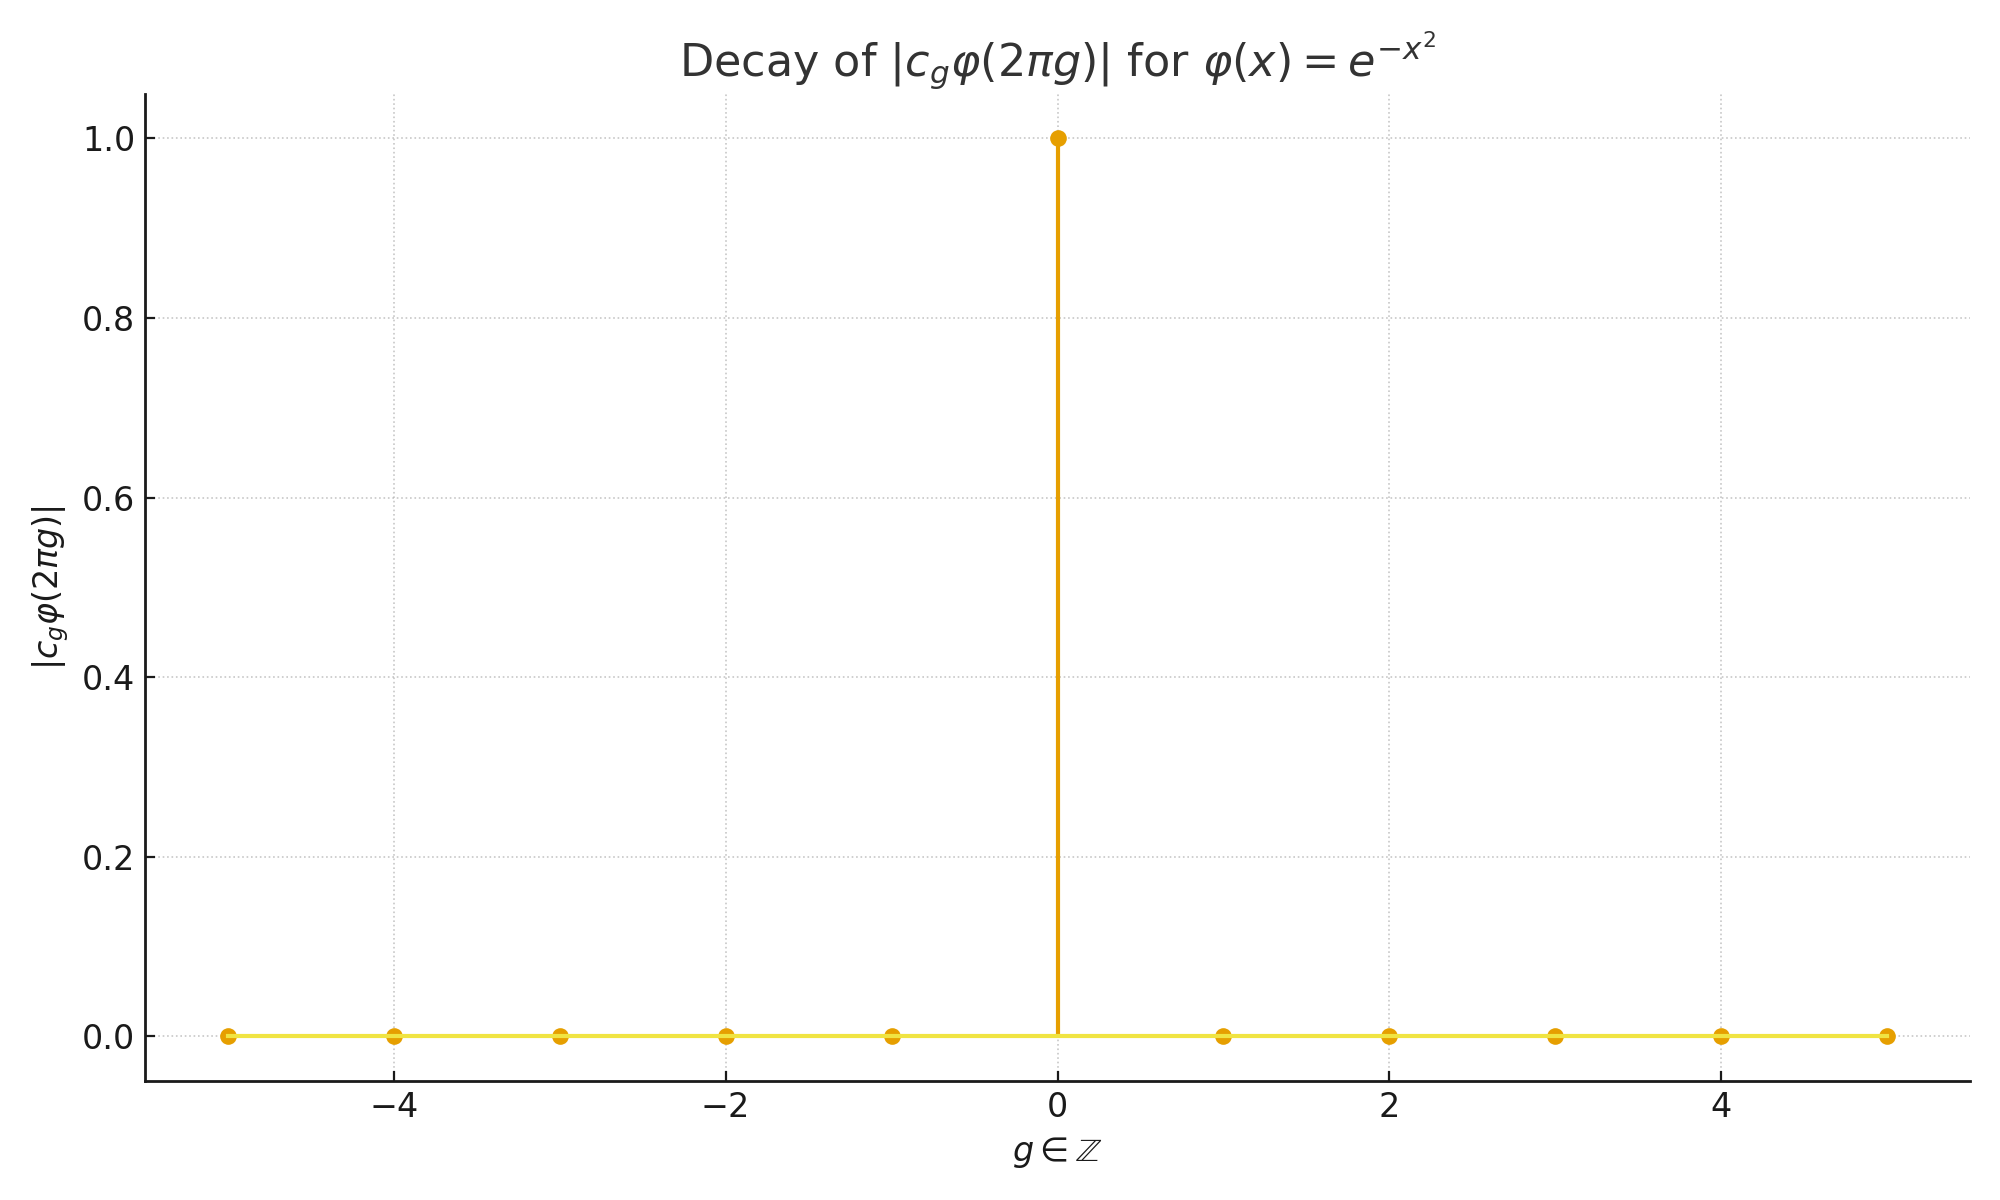
\includegraphics[width=0.8\textwidth]{figures/part03/fig_ex5-3-contributions.png}
\caption{The terms $|c_g\varphi(2\pi g)|$ for
$c_g=(1+|g|)^2$ and $\varphi(x)=e^{-x^2}$, illustrating
absolute convergence of the defining series.}
\label{fig:ex5-3-contributions}
\end{figure}

\begin{figure}[ht]
\centering
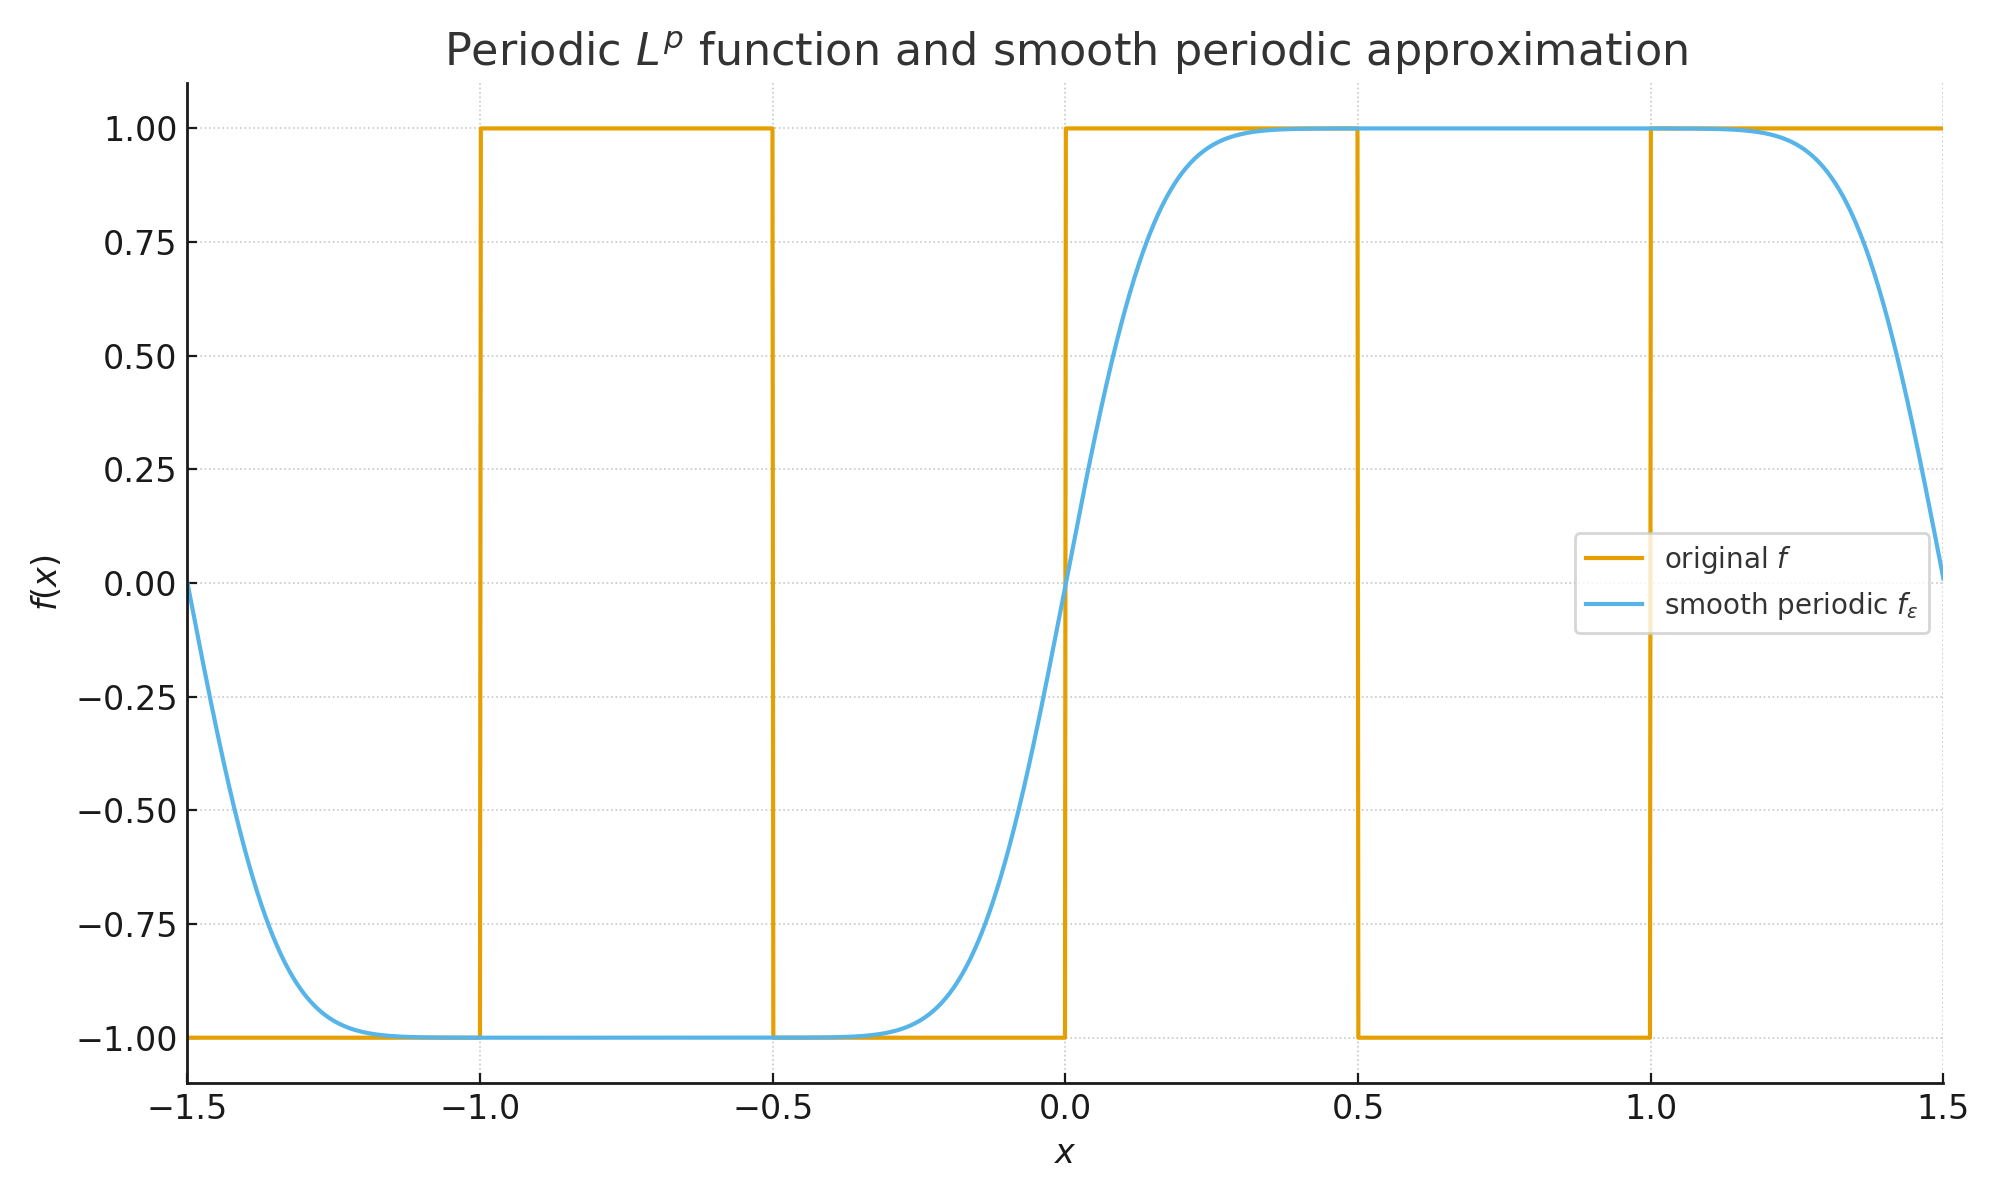
\includegraphics[width=0.8\textwidth]{figures/part03/fig_ex5-4-periodic-approx.png}
\caption{A periodic square wave $f$ and a smooth periodic
approximation $f_\varepsilon$ obtained by mollification.}
\label{fig:ex5-4-periodic-approx}
\end{figure}

\begin{figure}[ht]
\centering
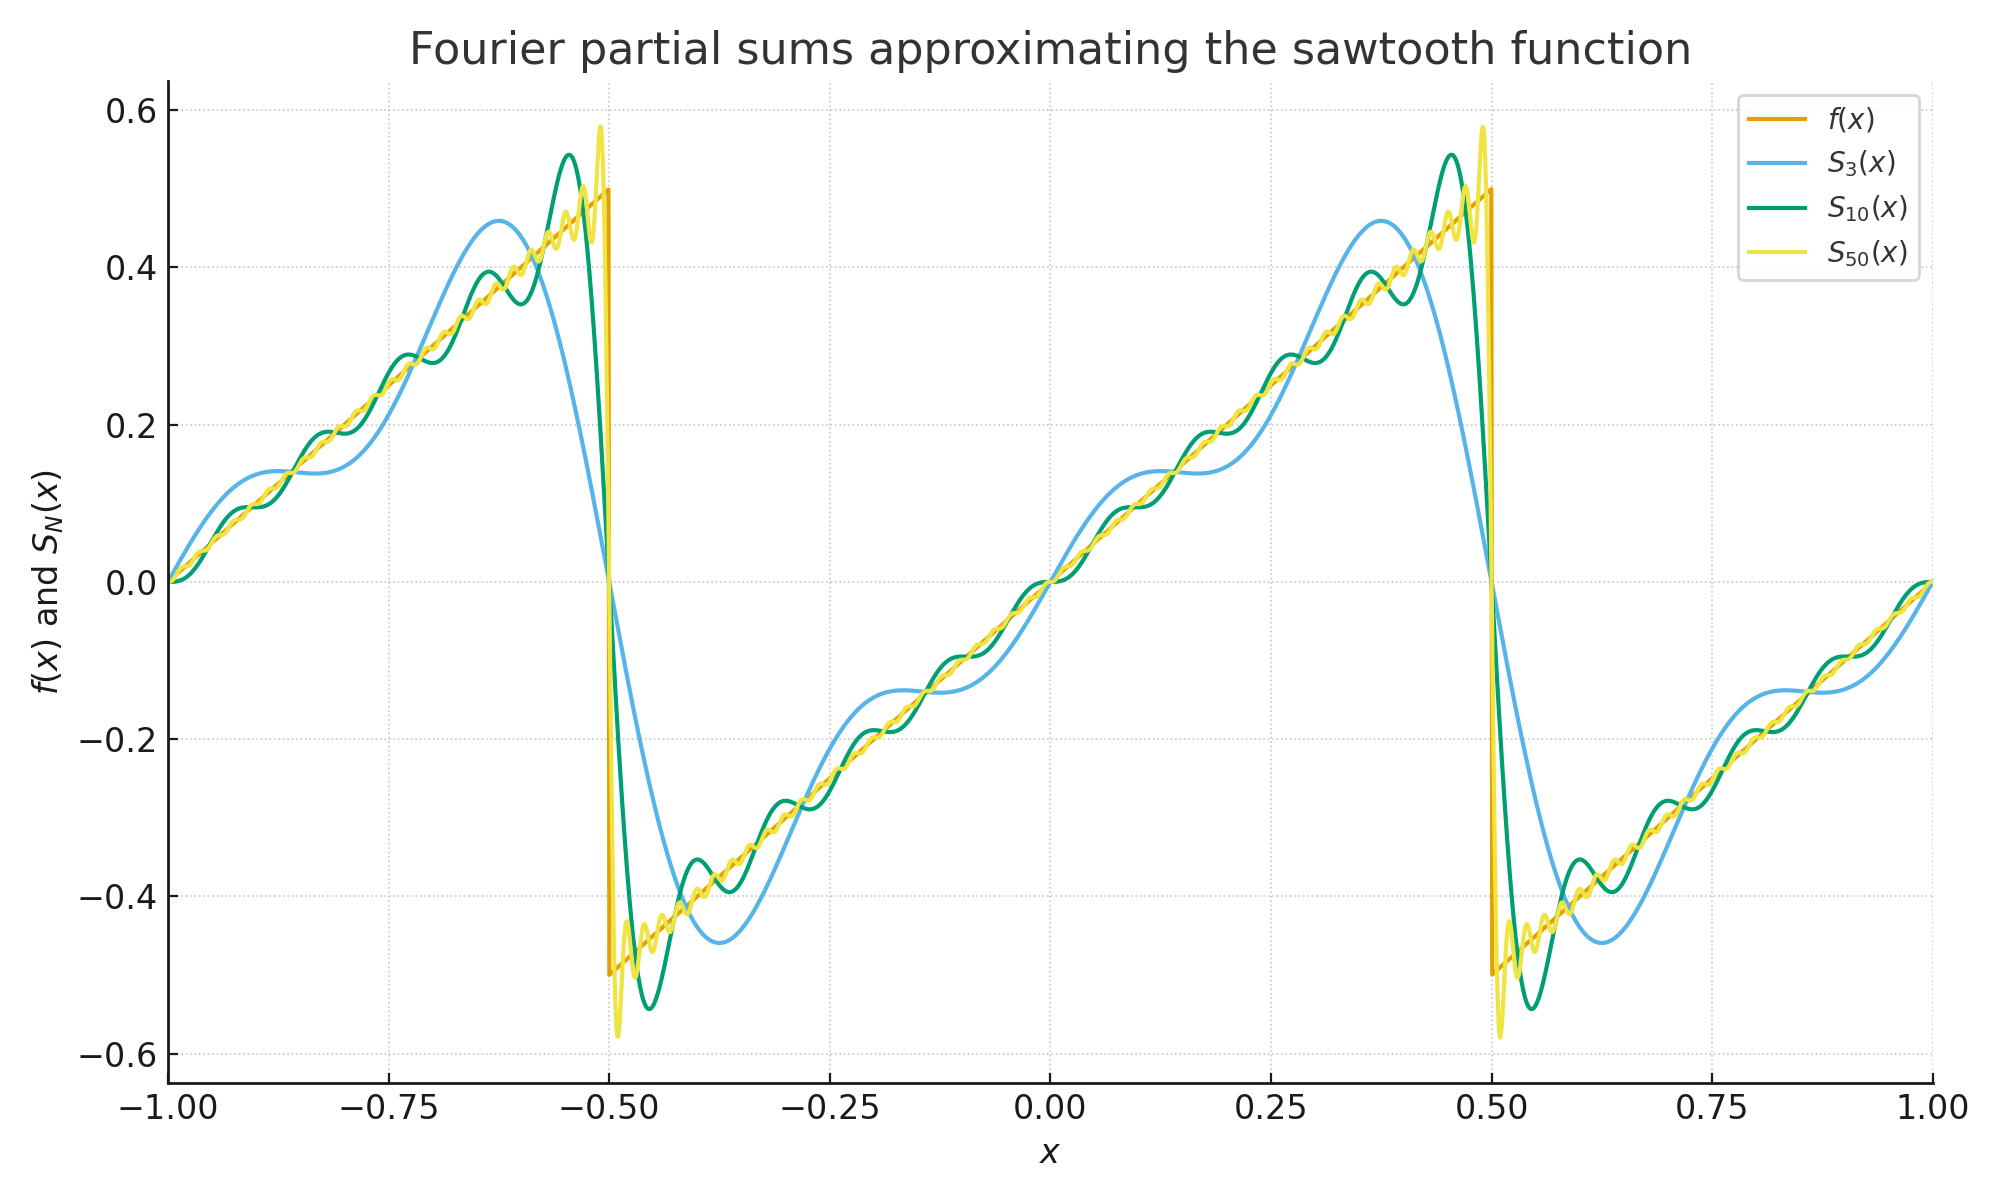
\includegraphics[width=0.8\textwidth]{figures/part03/fig_ex5-5-fourier-global.png}
\caption{Global comparison of the sawtooth function $f$ and partial
sums $S_N$ of its sine series for $N=3,10,50$.}
\label{fig:ex5-5-fourier-global}
\end{figure}

\begin{figure}[ht]
\centering
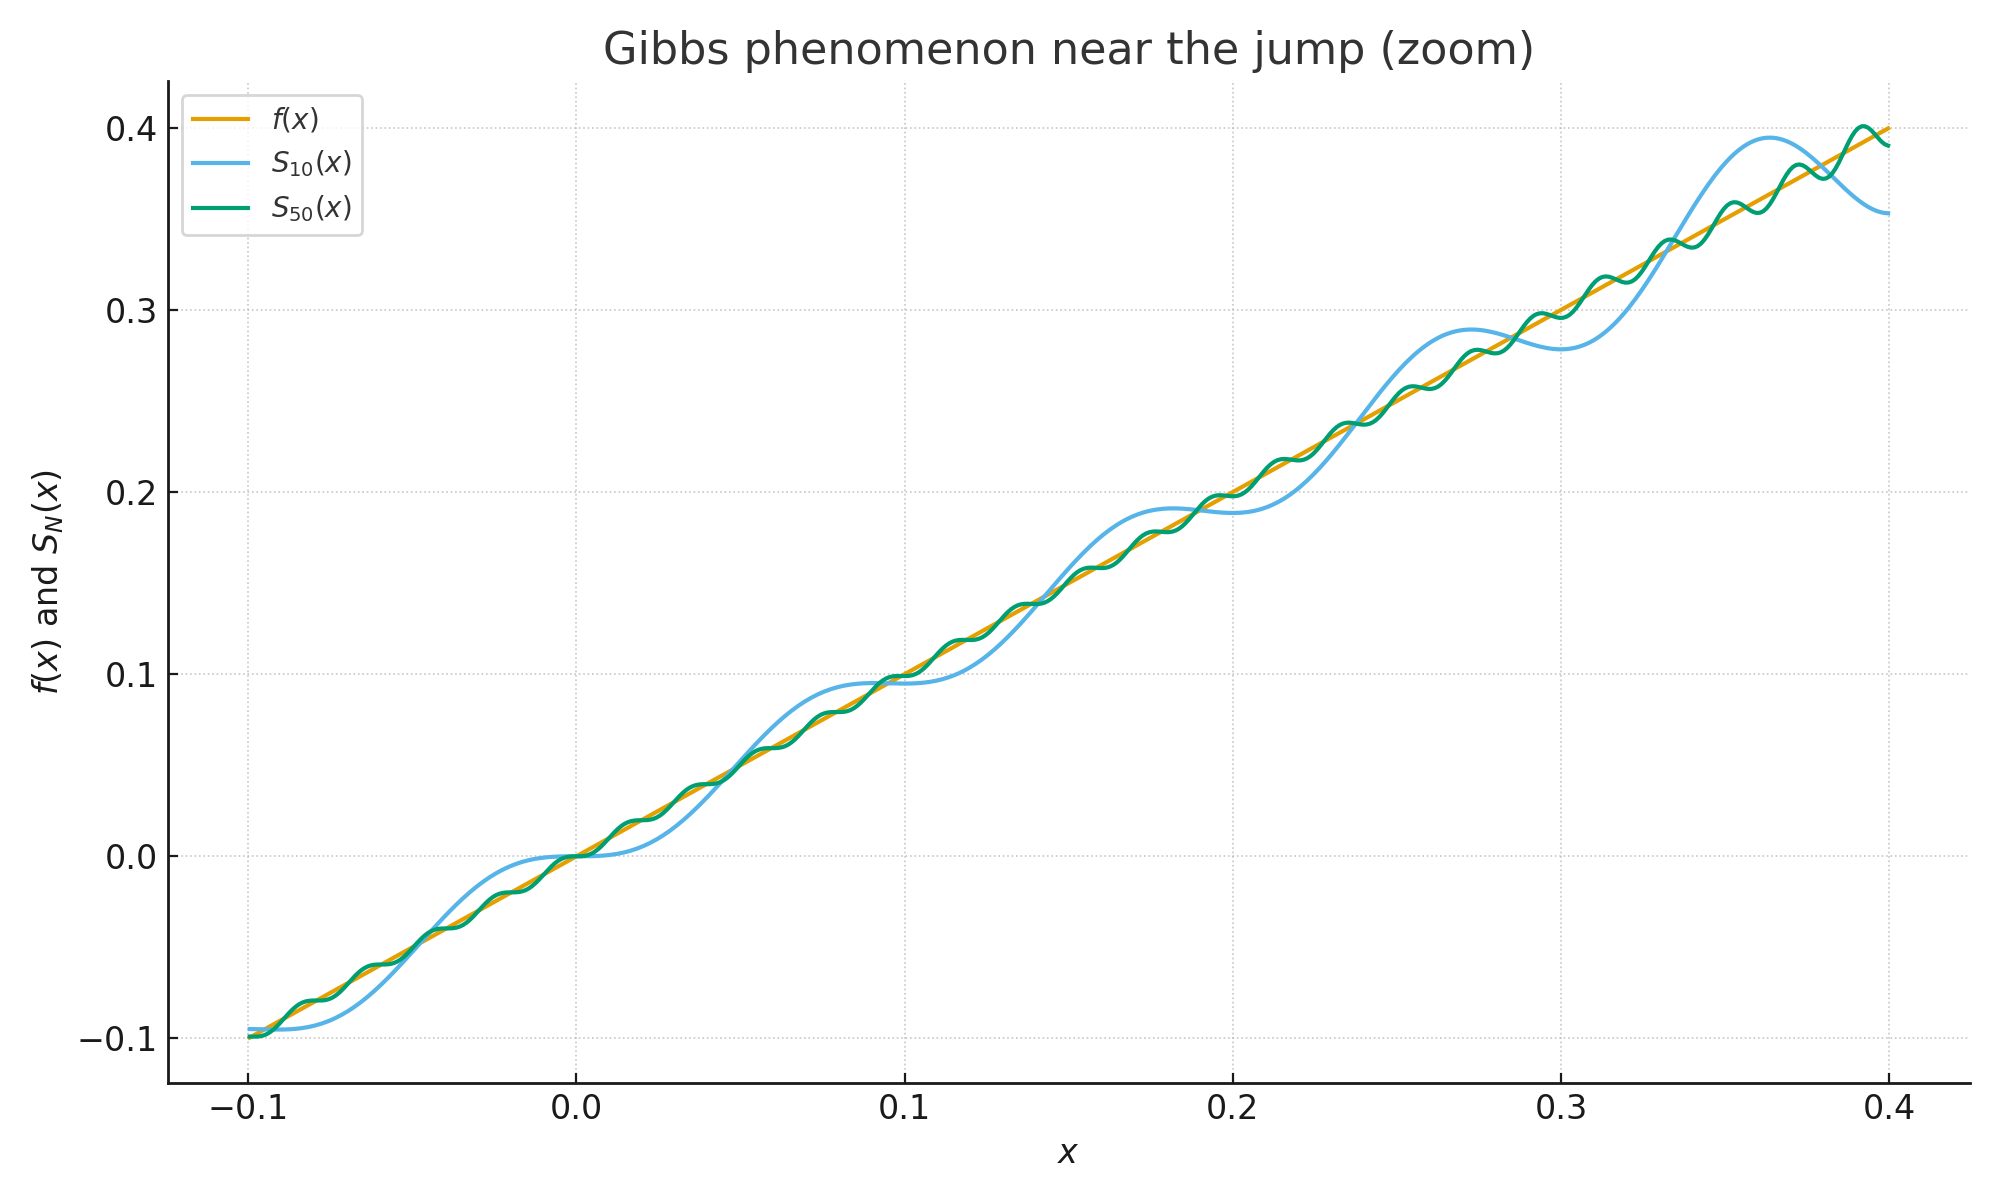
\includegraphics[width=0.8\textwidth]{figures/part03/fig_ex5-5-fourier-gibbs.png}
\caption{Zoom near a jump of the sawtooth function, showing the Gibbs
oscillations of the partial sums $S_{10}$ and $S_{50}$.}
\label{fig:ex5-5-fourier-gibbs}
\end{figure}
\end{problem}

\begin{solution}
\par\smallskip\noindent\textbf{(a) Weighted Dirac comb.}

For \(\varphi\in\mathcal S(\mathbb R)\), define
\[
T[\varphi]
=
\sum_{g\in\mathbb Z}
(1+|g|)^2\varphi(2\pi g).
\]
For every \(M\ge0\),
\[
|\varphi(x)|
\le
p_M(\varphi)(1+|x|)^{-M},
\]
where
\[
p_M(\varphi)
=
\sup_x
(1+|x|)^M|\varphi(x)|
\]
is a Schwartz seminorm. Hence
\[
\begin{aligned}
|T[\varphi]|
&\le
p_M(\varphi)
\sum_{g\in\mathbb Z}
(1+|g|)^2(1+2\pi|g|)^{-M}\\
&\le
C_M p_M(\varphi)
\sum_{g\in\mathbb Z}
(1+|g|)^{2-M}.
\end{aligned}
\]
Choose \(M>3\). The series converges, so
\[
|T[\varphi]|
\le
C\,p_M(\varphi).
\]
Thus \(T\) is a continuous linear functional on \(\mathcal S\):
\[
\boxed{
T\in\mathcal S'(\mathbb R).}
\]
This is the rigorous statement behind the weighted-comb contribution
figure.

\par\smallskip\noindent\textbf{(b) Periodic mollification.}

Because both \(f\) and \(\rho_\varepsilon\) are periodic,
\[
f_\varepsilon(x)
=
\int_{\mathbb T}
f(x-y)\rho_\varepsilon(y)\,dy
\]
is periodic. Differentiation falls on the smooth kernel:
\[
D^m f_\varepsilon
=
f*D^m\rho_\varepsilon,
\]
so \(f_\varepsilon\in C^\infty(\mathbb T)\).

Also,
\[
f*\rho_\varepsilon-f
=
\int_{\mathbb T}
\rho_\varepsilon(y)
\bigl(\tau_yf-f\bigr)\,dy.
\]
Minkowski gives
\[
\|f*\rho_\varepsilon-f\|_p
\le
\int
\rho_\varepsilon(y)
\|\tau_yf-f\|_p\,dy.
\]
Translations are continuous in \(L^p(\mathbb T)\), and the approximate
identity concentrates near \(y=0\). Therefore
\[
\boxed{
f*\rho_\varepsilon\to f
\quad\text{in }L^p(\mathbb T).}
\]

\par\smallskip\noindent\textbf{(c) Fourier partial sums and Gibbs.}

The periodic sawtooth belongs to \(L^2(\mathbb T)\). The trigonometric
system is complete in \(L^2\), so the orthogonal Fourier projections
satisfy
\[
\boxed{
\|S_N-f\|_{L^2(\mathbb T)}
\longrightarrow0.}
\]

The sawtooth is piecewise \(C^1\). By the Dirichlet convergence theorem,
at every continuity point \(x\),
\[
S_N(x)\to f(x),
\]
while at a jump point \(x_0\),
\[
S_N(x_0)
\to
\frac{f(x_0^-)+f(x_0^+)}2.
\]

Pointwise convergence at the jump does not imply uniform convergence near
the jump. After rescaling a shrinking neighborhood of \(x_0\), the
partial sums approach the universal sine-integral transition profile. Its
first maximum lies strictly above the upper one-sided value by a fixed
positive fraction of the jump. Consequently the spatial width of the
oscillatory region shrinks like \(N^{-1}\), but the relative overshoot does
not tend to zero.

That persistent nonzero overshoot is the Gibbs phenomenon shown in the
zoomed figure.

Thus the source figures represent, respectively,
\[
\boxed{
\text{Schwartz decay beats polynomial weights},
}
\]
\[
\boxed{
\text{periodic mollification gives smooth }L^p\text{-approximation},
}
\]
and
\[
\boxed{
\text{Fourier partial sums converge in }L^2
\text{ while retaining Gibbs overshoot near jumps}.}
\]
\end{solution}


\begin{problem}[CP-III-0019]
\label{prob:cp-iii-0019}
Suppose that $u_0 \in \mathscr{S}(\mathbb{R}^n)$.
	Show that for $t>0$:
	\[
	u(t,x) = \int_{\mathbb{R}^n} u_0(y)\, K_t(x-y)\, dy,
	\]
	and deduce the dispersive estimate
	\[
	\sup_{x\in\mathbb{R}^n} |u(t,x)|
	\;\;\lesssim\;\;
	\frac{1}{(4\pi t)^{n/2}}\, \|u_0\|_{L^1(\mathbb{R}^n)}.
	\]
	(This type of estimate shows the decay of solutions to the Schrödinger equation.)


\par\medskip\noindent\textbf{Schrödinger Equation in $\mathbb{R}^n$ : Theory and Solutions}\quad

Recall that for $s\ge 0$ the Sobolev norm is
\[
\|f\|_{H^s(\mathbb{R}^n)}^2
= \int_{\mathbb{R}^n} (1+|\xi|^2)^s |\widehat{f}(\xi)|^2\,d\xi.
\]

% ---------- (a) ----------
\par\smallskip\noindent\textbf{(a) \; Existence, Uniqueness and Fourier Representation}\quad

\par\smallskip\noindent\textbf{\textbf{Idea.}}\quad
Take the Fourier transform in the spatial variable, which turns the PDE
\[
u_t = i\Delta u
\]
into an ODE in $t$ for each $\xi$.

\par\smallskip\noindent\textbf{\textbf{Derivation.}}\quad
Using $\widehat{\Delta u}(t,\xi) = -|\xi|^2\widehat{u}(t,\xi)$, we get
\[
\partial_t \widehat{u}(t,\xi) = i\widehat{\Delta u}(t,\xi)
= -i|\xi|^2\,\widehat{u}(t,\xi), \qquad
\widehat{u}(0,\xi) = \widehat{u_0}(\xi).
\]
Hence
\[
\widehat{u}(t,\xi)
= e^{-it|\xi|^2}\,\widehat{u_0}(\xi).
\]

\par\smallskip\noindent\textbf{\textbf{Regularity.}}\quad
Define
\[
u(t,x)
:= \frac{1}{(2\pi)^n} \int_{\mathbb{R}^n}
\widehat{u_0}(\xi)\,e^{-it|\xi|^2} e^{ix\cdot\xi}\,d\xi.
\]
Since $u_0\in H^2(\mathbb{R}^n)$, we have
$(1+|\xi|^2)^2\widehat{u_0}(\xi)\in L^2$, and the multiplier
$e^{-it|\xi|^2}$ is bounded for each $t$. Standard Fourier multiplier
arguments give
\[
u \in C^0([0,T];H^2(\mathbb{R}^n))
\cap C^1((0,T);L^2(\mathbb{R}^n)).
\]

\par\smallskip\noindent\textbf{\textbf{Uniqueness.}}\quad
If $v$ is another solution with the same regularity and $v(0)=u_0$, then
$\widehat{v}$ satisfies the same ODE with the same initial data and
hence $\widehat{v}=\widehat{u}$. Thus $v=u$ and the solution is unique.

\medskip
In particular,
\[
\widehat{u}(t,\xi) = \widehat{u_0}(\xi)\,e^{-it|\xi|^2},
\]
as required.

% ---------- (b) ----------
\par\smallskip\noindent\textbf{(b) \; Conservation of the $H^2$-norm}\quad

\par\smallskip\noindent\textbf{\textbf{Computation.}}\quad
Using the formula from part~(a),
\[
\|u(t,\cdot)\|_{H^2}^2
= \int_{\mathbb{R}^n} (1+|\xi|^2)^2\,|\widehat{u}(t,\xi)|^2\,d\xi
= \int (1+|\xi|^2)^2\,|e^{-it|\xi|^2}|^2\,|\widehat{u_0}(\xi)|^2\,d\xi.
\]
Since $|e^{-it|\xi|^2}|=1$,
\[
\|u(t,\cdot)\|_{H^2}^2
= \int (1+|\xi|^2)^2 |\widehat{u_0}(\xi)|^2\,d\xi
= \|u_0\|_{H^2}^2.
\]
Hence
\[
\|u(t,\cdot)\|_{H^2(\mathbb{R}^n)} = \|u_0\|_{H^2(\mathbb{R}^n)}
\quad \text{for all } t\in[0,T].
\]

% ---------- (c) ----------
\par\smallskip\noindent\textbf{(c) \; The Schrödinger Kernel $K_t$ and its Fourier Transform}\quad

For $t>0$, set
\[
K_t(x) := \frac{1}{(4\pi i t)^{n/2}} e^{\, i|x|^2 /4t},
\qquad
K_t^\varepsilon(x) := e^{-\varepsilon|x|^2}K_t(x),\quad \varepsilon>0.
\]

\par\smallskip\noindent\textbf{\textbf{(i) Convergence in $\mathscr{S}'$.}}\quad
Let $\varphi\in\mathscr{S}(\mathbb{R}^n)$. Then
\[
\langle T_{K_t^\varepsilon},\varphi\rangle
= \int_{\mathbb{R}^n} K_t(x)\,e^{-\varepsilon|x|^2}\,\varphi(x)\,dx.
\]
As $\varepsilon\to0$, $e^{-\varepsilon|x|^2}\to1$ pointwise, and
\[
|K_t(x)e^{-\varepsilon|x|^2}\varphi(x)|
\le |K_t(x)\varphi(x)|.
\]
Since $K_t$ has at most polynomial growth and $\varphi$ is rapidly
decreasing, $K_t\varphi\in L^1(\mathbb{R}^n)$, so dominated convergence
gives
\[
\langle T_{K_t^\varepsilon},\varphi\rangle
\longrightarrow \int K_t(x)\varphi(x)\,dx
= \langle T_{K_t},\varphi\rangle.
\]
Thus $T_{K_t^\varepsilon}\to T_{K_t}$ in $\mathscr{S}'$.

\par\smallskip\noindent\textbf{\textbf{(ii) Complex Gaussian integral.}}\quad
If $\Re(\sigma)>0$, then
\[
\int_{\mathbb{R}} e^{-\sigma x^2 - i\xi x}\,dx
= \sqrt{\frac{\pi}{\sigma}}\, e^{-\xi^2/(4\sigma)}.
\]
This follows by completing the square and deforming the integration path.

\par\smallskip\noindent\textbf{\textbf{(iii) Fourier transform of $K_t^\varepsilon$.}}\quad
We write
\[
K_t^\varepsilon(x)
= \frac{1}{(4\pi i t)^{n/2}}\exp\!\Bigl(-\sigma |x|^2\Bigr),
\qquad
\sigma := \varepsilon - \frac{i}{4t},\quad \Re(\sigma)>0.
\]
Using (ii) in each coordinate, we obtain
\[
\widehat{e^{-\sigma |x|^2}}(\xi)
= \left(\sqrt{\frac{\pi}{\sigma}}\right)^n
\exp\!\Bigl(-\frac{|\xi|^2}{4\sigma}\Bigr),
\]
hence
\[
\widehat{K_t^\varepsilon}(\xi)
= \frac{1}{(4\pi i t)^{n/2}}
\left(\frac{\pi}{\sigma}\right)^{n/2}
\exp\!\Bigl(-\frac{|\xi|^2}{4\sigma}\Bigr).
\]
A straightforward simplification yields
\[
\widehat{K_t^\varepsilon}(\xi)
= \bigl(1+4it\varepsilon\bigr)^{-n/2}
\exp\!\left(-\frac{it|\xi|^2}{1+4it\varepsilon}\right).
\]

\par\smallskip\noindent\textbf{\textbf{(iv) Limit as $\varepsilon\to0$.}}\quad
As $\varepsilon\to0$,
\[
1+4it\varepsilon \to 1,
\qquad
-\frac{it|\xi|^2}{1+4it\varepsilon} \to -it|\xi|^2.
\]
Thus
\[
\widehat{K_t^\varepsilon}(\xi) \longrightarrow e^{-it|\xi|^2}
\quad\text{pointwise in }\xi.
\]
By (i), $T_{K_t^\varepsilon}\to T_{K_t}$ in $\mathscr{S}'$ and the
Fourier transform is continuous on $\mathscr{S}'$, so we conclude
\[
\widehat{K_t}(\xi) = e^{-it|\xi|^2}.
\]

% ---------- (d) ----------
\par\smallskip\noindent\textbf{(d) \; Convolution Representation and Dispersive Estimate}\quad

Assume $u_0\in\mathscr{S}(\mathbb{R}^n)$. From part~(a),
\[
\widehat{u}(t,\xi) = e^{-it|\xi|^2}\,\widehat{u_0}(\xi),
\]
and from part~(c),
\[
\widehat{K_t}(\xi) = e^{-it|\xi|^2}.
\]
Hence
\[
\widehat{u}(t,\xi)
= \widehat{u_0}(\xi)\,\widehat{K_t}(\xi)
= \mathcal{F}(u_0 * K_t)(\xi),
\]
so by injectivity of the Fourier transform
\[
u(t,x) = (u_0 * K_t)(x)
= \int_{\mathbb{R}^n} u_0(y)\,K_t(x-y)\,dy.
\]

\par\smallskip\noindent\textbf{\textbf{Dispersive estimate.}}\quad
Since $|e^{i|z|^2/(4t)}| = 1$, we have
\[
|K_t(z)| = \frac{1}{(4\pi |t|)^{n/2}}
\quad\text{for all } z\in\mathbb{R}^n.
\]
Then
\[
|u(t,x)|
\le \int_{\mathbb{R}^n} |u_0(y)|\,|K_t(x-y)|\,dy
\le \frac{1}{(4\pi|t|)^{n/2}} \int_{\mathbb{R}^n} |u_0(y)|\,dy.
\]
Taking the supremum over $x\in\mathbb{R}^n$ yields
\[
\sup_{x\in\mathbb{R}^n} |u(t,x)|
\le \frac{1}{(4\pi|t|)^{n/2}}\,\|u_0\|_{L^1(\mathbb{R}^n)}.
\]

\par\smallskip\noindent\textbf{\textbf{Conclusion.}}\quad
The free Schrödinger evolution is given by
$u(t,\cdot)=e^{it\Delta}u_0=u_0*K_t$,
acts unitarily on $H^2(\mathbb{R}^n)$, and satisfies the dispersive
estimate above, which shows decay in $L^\infty$ for data in $L^1$.

\par\medskip\noindent\textbf{Sobolev Space $H^{s}(\mathbb{R}^n)$ used in Exercise 5.10}\quad

Throughout this section, $H^{s}(\mathbb{R}^n)$ denotes the $L^2$-based Sobolev
space. For $s \ge 0$ we define
\[
H^{s}(\mathbb{R}^n)
:= \Bigl\{ f \in \mathscr{S}'(\mathbb{R}^n)
: \int_{\mathbb{R}^n} (1+|\xi|^2)^s |\widehat{f}(\xi)|^2 \, d\xi
< \infty \Bigr\},
\]
with norm
\[
\|f\|_{H^{s}(\mathbb{R}^n)}^2
:= \int_{\mathbb{R}^n} (1+|\xi|^2)^s |\widehat{f}(\xi)|^2 \, d\xi.
\]

For integer $s = m \in \mathbb{N}$ this is equivalent to
\[
H^{m}(\mathbb{R}^n)
= \Bigl\{ f \in L^2(\mathbb{R}^n)
: D^\alpha f \in L^2(\mathbb{R}^n) \text{ for all } |\alpha|\le m \Bigr\},
\]
and
\[
\|f\|_{H^{m}(\mathbb{R}^n)}^2
\simeq \sum_{|\alpha|\le m} \|D^\alpha f\|_{L^2(\mathbb{R}^n)}^2.
\]

In particular, in Exercise~5.10 the assumption $u_0 \in H^2(\mathbb{R}^n)$
means that $u_0$ and all second-order derivatives of $u_0$ belong to
$L^2(\mathbb{R}^n)$, and the solution $u(t,\cdot)$ stays in $H^2$ for all
times $t$.


\par\medskip\noindent\textbf{Relation Between Sobolev Spaces and the Schwartz Space}\quad

Let $\mathscr{S}(\mathbb{R}^n)$ denote the Schwartz space of rapidly
decreasing smooth functions. Recall that for $s\in\mathbb{R}$ the
$L^2$--based Sobolev space $H^s(\mathbb{R}^n)$ is defined by
\[
H^s(\mathbb{R}^n)
:= \Bigl\{ f\in\mathscr{S}'(\mathbb{R}^n) :
\int_{\mathbb{R}^n} (1+|\xi|^2)^s \,|\widehat{f}(\xi)|^2 \, d\xi
< \infty \Bigr\}.
\]

\par\smallskip\noindent\textbf{Inclusion.}\quad
Since $\widehat{f}\in\mathscr{S}(\mathbb{R}^n)$ whenever
$f\in\mathscr{S}(\mathbb{R}^n)$, the quantity
$(1+|\xi|^2)^s|\widehat{f}(\xi)|^2$ decays faster than any power of
$|\xi|$. Hence
\[
\mathscr{S}(\mathbb{R}^n) \subset H^s(\mathbb{R}^n)
\quad\text{for all } s\in\mathbb{R}.
\]

\par\smallskip\noindent\textbf{Density.}\quad
For every $s\in\mathbb{R}$ the Schwartz space is dense in $H^s$:
\[
\overline{\mathscr{S}(\mathbb{R}^n)}^{\,H^s(\mathbb{R}^n)}
= H^s(\mathbb{R}^n).
\]
This follows from approximation by mollifiers and compactly supported
smooth functions, as in Exercise~5.8.

\par\smallskip\noindent\textbf{Intersection over all orders.}\quad
One has the characterization
\[
\mathscr{S}(\mathbb{R}^n)
= \bigcap_{s\in\mathbb{R}} H^s(\mathbb{R}^n),
\]
that is, a tempered distribution belongs to the Schwartz space if and
only if it lies in every Sobolev space $H^s(\mathbb{R}^n)$.

\par\smallskip\noindent\textbf{Remark.}\quad
The space
\[
H^\infty(\mathbb{R}^n)
:= \bigcap_{m\in\mathbb{N}} H^m(\mathbb{R}^n)
\]
consists of functions with all derivatives in $L^2$ and contains
$\mathscr{S}(\mathbb{R}^n)$ as a dense subspace. The additional
requirement that both $f$ and $\widehat{f}$ decay faster than any power
of $|x|$ and $|\xi|$ is what distinguishes the Schwartz space from
general elements of $H^\infty$.


\par\medskip\noindent\textbf{Exercise 5.11 : Radial Solutions of the Wave Equation in $\mathbb{R}^3$}\quad

Let $\mathbb{R}^3_* := \mathbb{R}^3\setminus\{0\}$ and
\[
S_{*,T} := (-T,T)\times\mathbb{R}^3_*,
\qquad
S_T := (-T,T)\times\mathbb{R}^3,
\qquad
\Sigma_0 := \{0\}\times\mathbb{R}^3.
\]
Write $r = |x|$. You may assume the formula for radial functions
$u=u(r,t)$:
\[
\Delta u(|x|,t) = \Delta u(r,t)
= \frac{\partial^2 u}{\partial r^2}(r,t)
+ \frac{2}{r}\frac{\partial u}{\partial r}(r,t).
\]

We consider the wave equation
\[
-\,\frac{\partial^2 u}{\partial t^2}(x,t)
+ \Delta u(x,t) = 0.
\]

\end{problem}

\begin{solution}
Taking the spatial Fourier transform of
\[
u_t=i\Delta u,
\qquad
u(0)=u_0,
\]
gives
\[
\partial_t\widehat u(t,\xi)
=
-i|\xi|^2\widehat u(t,\xi),
\]
so
\[
\widehat u(t,\xi)
=
e^{-it|\xi|^2}\widehat{u_0}(\xi).
\]
Let
\[
K_t(x)
=
\frac1{(4\pi it)^{n/2}}
e^{\,i|x|^2/(4t)}
\qquad(t>0).
\]
Its Fourier transform is
\[
\widehat K_t(\xi)=e^{-it|\xi|^2}.
\]
Hence
\[
\widehat u(t,\xi)
=
\widehat{u_0}(\xi)\widehat K_t(\xi),
\]
and injectivity of the Fourier transform gives
\[
\boxed{
u(t,x)
=
(u_0*K_t)(x)
=
\int_{\mathbb R^n}u_0(y)K_t(x-y)\,dy.
}
\]

Since
\[
|K_t(x)|
=
\frac1{(4\pi t)^{n/2}},
\]
we obtain
\[
|u(t,x)|
\le
\frac1{(4\pi t)^{n/2}}
\int_{\mathbb R^n}|u_0(y)|\,dy.
\]
Therefore
\[
\boxed{
\|u(t,\cdot)\|_\infty
\le
\frac1{(4\pi t)^{n/2}}
\|u_0\|_1.
}
\]
This is the free Schrödinger dispersive estimate requested in the
problem.

The additional Sobolev discussion in the migrated body is compatible
with this Fourier representation, but it is not needed for the stated
convolution and decay estimate.
\end{solution}


\begin{problem}[CP-III-0022]
\label{prob:cp-iii-0022}
Consider the ODE
\begin{equation}
	-\phi''(x) + \phi(x) = f(x), \qquad f:\mathbb{R}\to\mathbb{C}.
\end{equation}

\par\smallskip\noindent\textbf{(a)}\quad
Assume $f\in\mathcal{S}(\mathbb{R})$.
Taking the Fourier transform of both sides gives
\[
\widehat{-\phi'' + \phi}(\xi)
= -\,\widehat{\phi''}(\xi) + \widehat{\phi}(\xi).
\]

Using the standard identities
\[
\widehat{g'}(\xi) = (2\pi i\xi)\,\widehat{g}(\xi),
\qquad
\widehat{g''}(\xi) = -(2\pi\xi)^{2}\widehat{g}(\xi)
= -4\pi^{2}\xi^{2}\widehat{g}(\xi),
\]
we obtain
\[
-\widehat{\phi''}(\xi) + \widehat{\phi}(\xi)
= 4\pi^{2}\xi^{2}\widehat{\phi}(\xi) + \widehat{\phi}(\xi)
= (4\pi^{2}\xi^{2} + 1)\widehat{\phi}(\xi).
\]

Thus the transformed equation is
\[
(4\pi^{2}\xi^{2} + 1)\,\widehat{\phi}(\xi) = \widehat{f}(\xi),
\]
and hence
\[
\boxed{
	\widehat{\phi}(\xi)
	= \frac{\widehat{f}(\xi)}{1 + 4\pi^{2}\xi^{2}}.
}
\]

Since the multiplier $(1+4\pi^{2}\xi^{2})^{-1}$ is smooth and rapidly decaying,
multiplication by it preserves the Schwartz class.
Thus $\phi\in\mathcal{S}(\mathbb{R})$.

The homogeneous equation $-\psi''+\psi=0$ has solutions
$\psi(x)=Ce^{x}+De^{-x}$, none of which lie in $\mathcal{S}$ unless $C=D=0$.
Hence the solution in $\mathcal{S}$ is unique.

\par\smallskip\noindent\textbf{(b)}\quad
Define the Green's function
\[
G(x) =
\begin{cases}
	\frac12 e^{x}, & x<0,\\[0.3em]
	\frac12 e^{-x}, & x\ge 0.
\end{cases}
\]
A direct calculation yields
\[
\widehat{G}(\xi)
= \frac{1}{1+4\pi^{2}\xi^{2}}.
\]
Thus from part (a),
\[
\widehat{\phi}(\xi)
= \widehat{f}(\xi)\,\widehat{G}(\xi)
= \widehat{\,f*G\,}(\xi).
\]
By injectivity of the Fourier transform,
\[
\boxed{
	\phi(x) = (f*G)(x)
	= \int_{\mathbb{R}} f(y)\,G(x-y)\,dy.
}
\]
\end{problem}

\begin{solution}
Fourier transformation gives
\[
\widehat{-\phi''+\phi}(\xi)
=
(1+4\pi^2\xi^2)\widehat\phi(\xi),
\]
so
\[
\boxed{
\widehat\phi(\xi)
=
\frac{\widehat f(\xi)}{1+4\pi^2\xi^2}.
}
\]
Because multiplication by the smooth symbol
\((1+4\pi^2\xi^2)^{-1}\) preserves the Schwartz class,
\(f\in\mathcal S\) implies \(\phi\in\mathcal S\).

Now define
\[
G(x)=\frac12e^{-|x|}.
\]
One checks distributionally that
\[
-G''+G=\delta_0.
\]
Equivalently,
\[
\widehat G(\xi)
=
\frac1{1+4\pi^2\xi^2}.
\]
Therefore
\[
\widehat\phi
=
\widehat f\,\widehat G
=
\widehat{f*G},
\]
and hence
\[
\boxed{
\phi(x)
=
(f*G)(x)
=
\frac12\int_{\mathbb R}f(y)e^{-|x-y|}\,dy.
}
\]

If two Schwartz solutions existed, their difference would satisfy
\[
-\psi''+\psi=0,
\]
so \(\psi=Ce^x+De^{-x}\).  The only such Schwartz function is \(0\), and
the solution is unique.
\end{solution}


\begin{problem}[CP-III-0023]
\label{prob:cp-iii-0023}
\textbf{\(\Lambda\)-periodic distributions and the Fourier dual lattice.}

Let
\[
\lambda=\{\lambda_1,\dots,\lambda_n\}
\]
be a basis of \(\mathbb R^n\), and let
\[
\Lambda
=
\left\{
\sum_{j=1}^n z_j\lambda_j:
z_j\in\mathbb Z
\right\}.
\]
Write
\[
q_\Lambda
=
\left\{
\sum_{j=1}^n x_j\lambda_j:
|x_j|<\frac12
\right\}.
\]
A distribution \(u\in\mathcal D'(\mathbb R^n)\) is
\(\Lambda\)-periodic if
\[
\tau_g u=u
\qquad(g\in\Lambda).
\]

\par\smallskip\noindent\textbf{(a)}
Show that there exists
\[
\psi\in C_c^\infty(2q_\Lambda),
\qquad
\psi\ge0,
\]
such that
\[
\sum_{g\in\Lambda}\tau_g\psi=1.
\]

\par\smallskip\noindent\textbf{(b)}
If \(u\) is \(\Lambda\)-periodic and \(\psi,\psi'\) both satisfy part~(a),
show that
\[
\frac1{|q_\Lambda|}u[\psi]
=
\frac1{|q_\Lambda|}u[\psi'].
\]
Hence
\[
M(u)
:=
\frac1{|q_\Lambda|}u[\psi]
\]
is well defined.

\par\smallskip\noindent\textbf{(c) Fourier dual lattice.}
Let \(\mu_1,\dots,\mu_n\) be the Euclidean dual basis:
\[
\mu_j\cdot\lambda_k=\delta_{jk}.
\]
Define
\[
\lambda_j^*
=
2\pi\mu_j.
\]
Show that
\[
\lambda_j^*\cdot\lambda_k
=
2\pi\delta_{jk}
\]
and that the Fourier dual lattice
\[
\Lambda^*
=
\left\{
\xi\in\mathbb R^n:
g\cdot\xi\in2\pi\mathbb Z
\text{ for every }g\in\Lambda
\right\}
\]
is exactly
\[
\Lambda^*
=
\left\{
\sum_{j=1}^n m_j\lambda_j^*:
m_j\in\mathbb Z
\right\}.
\]

\par\smallskip\noindent\textbf{(d) Characters.}
For \(\xi\in\mathbb R^n\), set
\[
e_\xi(x)=e^{i\xi\cdot x}.
\]
Show that \(e_\xi\) is \(\Lambda\)-periodic whenever
\(\xi\in\Lambda^*\).

\par\smallskip\noindent\textbf{(e) Fourier transform.}
First show that every \(\Lambda\)-periodic distribution is tempered.
Then prove that
\[
\widehat u
=
\sum_{\xi\in\Lambda^*}
c_\xi\,\delta_\xi
\]
for coefficients satisfying
\[
|c_\xi|
\le
C(1+|\xi|)^N
\]
for some \(C>0\) and \(N\in\mathbb N_0\).

\par\smallskip\noindent\textbf{(f) Fourier series.}
Show that
\[
u
=
\sum_{\xi\in\Lambda^*}
d_\xi e_\xi
\]
in \(\mathcal S'(\mathbb R^n)\), where the coefficients have polynomial
growth and
\[
d_\xi
=
M(e_{-\xi}u).
\]

\medskip
\noindent
\textit{Source correction.}
The migrated source defined \(\Lambda^*\) using
\(2\pi\mathbb Z\) but simultaneously asked for generators satisfying
\(\lambda_j^*\cdot\lambda_k=\delta_{jk}\). The formulation above
distinguishes the algebraic dual basis \(\mu_j\) from the Fourier dual
basis \(2\pi\mu_j\).
\end{problem}

\begin{solution}
We use the convention
\[
(\tau_g\varphi)(x)=\varphi(x-g).
\]
If \(u\) is \(\Lambda\)-periodic, then
\[
u[\tau_g\varphi]=u[\varphi]
\qquad(g\in\Lambda)
\]
for every test function \(\varphi\).

\par\smallskip\noindent\textbf{(a) Partition of unity.}
Choose
\[
\chi\in C_c^\infty(2q_\Lambda),
\qquad
\chi\ge0,
\]
with \(\chi>0\) on \(\overline{q_\Lambda}\). Define
\[
S(x)
=
\sum_{g\in\Lambda}
(\tau_g\chi)(x).
\]
The sum is locally finite, hence \(S\) is smooth. It is
\(\Lambda\)-periodic, and it is strictly positive because the translates
of \(\overline{q_\Lambda}\) cover \(\mathbb R^n\). Set
\[
\psi(x)=\frac{\chi(x)}{S(x)}.
\]
Then
\[
\psi\in C_c^\infty(2q_\Lambda),
\qquad
\psi\ge0,
\]
and, because \(S(x-g)=S(x)\),
\[
\sum_{g\in\Lambda}\tau_g\psi(x)
=
\frac1{S(x)}
\sum_{g\in\Lambda}\tau_g\chi(x)
=
1.
\]

\par\smallskip\noindent\textbf{(b) Independence of the cutoff.}
Let
\[
\rho=\psi-\psi'.
\]
Then
\[
\sum_{g\in\Lambda}\tau_g\rho=0.
\]
Using the partition of unity generated by \(\psi\), and noting that only
finitely many terms meet the compact support of \(\rho\),
\[
u[\rho]
=
\sum_{g\in\Lambda}
u[\rho\,\tau_g\psi].
\]
Periodicity lets us shift each summand back to the fixed cell:
\[
u[\rho\,\tau_g\psi]
=
u[\tau_{-g}(\rho\,\tau_g\psi)]
=
u[(\tau_{-g}\rho)\psi].
\]
Therefore
\[
\begin{aligned}
u[\rho]
&=
u\left[
\psi
\sum_{g\in\Lambda}\tau_{-g}\rho
\right]\\
&=0,
\end{aligned}
\]
because \(-\Lambda=\Lambda\). Hence
\[
u[\psi]=u[\psi'],
\]
so \(M(u)\) is well defined.

\par\smallskip\noindent\textbf{(c) The \(2\pi\)-normalized dual lattice.}
Let \(L\) be the matrix whose columns are
\(\lambda_1,\dots,\lambda_n\). The Euclidean dual basis has columns
\[
L^{-T},
\]
so
\[
\mu_j\cdot\lambda_k=\delta_{jk}.
\]
Put
\[
\lambda_j^*=2\pi\mu_j.
\]
Then
\[
\lambda_j^*\cdot\lambda_k
=
2\pi\delta_{jk}.
\]

If
\[
\xi=\sum_j a_j\mu_j,
\]
then
\[
\lambda_k\cdot\xi=a_k.
\]
Thus
\[
\xi\in\Lambda^*
\iff
a_k\in2\pi\mathbb Z
\quad\text{for every }k.
\]
Consequently
\[
\boxed{
\Lambda^*
=
\left\{
\sum_{j=1}^n
m_j\lambda_j^*:
m_j\in\mathbb Z
\right\}.
}
\]

\par\smallskip\noindent\textbf{(d) Periodic characters.}
If \(\xi\in\Lambda^*\) and \(g_0\in\Lambda\), then
\[
\xi\cdot g_0\in2\pi\mathbb Z.
\]
Hence
\[
e_\xi(x+g_0)
=
e^{i\xi\cdot x}
e^{i\xi\cdot g_0}
=
e_\xi(x).
\]

\par\smallskip\noindent\textbf{(e) Periodic distributions are tempered.}
Let \(\psi\) be as in part~(a), and let
\[
K=\operatorname{supp}\psi.
\]
Because \(u\in\mathcal D'\), there are \(m\in\mathbb N_0\) and \(C>0\)
such that, for every test function \(\eta\) supported in \(K\),
\[
|u[\eta]|
\le
C
\max_{|\alpha|\le m}
\sup_K |D^\alpha\eta|.
\]

For \(\varphi\in\mathcal S\), define
\[
U[\varphi]
=
\sum_{g\in\Lambda}
u[\varphi\,\tau_g\psi].
\]
Using periodicity,
\[
u[\varphi\,\tau_g\psi]
=
u[(\tau_{-g}\varphi)\psi].
\]
For every \(M\), the Schwartz seminorms imply
\[
\max_{|\alpha|\le m}
\sup_K
|D^\alpha((\tau_{-g}\varphi)\psi)|
\le
C_M
(1+|g|)^{-M}
p_{M,m}(\varphi),
\]
where \(p_{M,m}\) is a Schwartz seminorm. Choosing \(M>n\), the lattice
sum converges. Thus
\[
|U[\varphi]|
\le
C'
p_{M,m}(\varphi),
\]
so \(U\in\mathcal S'\). On compactly supported test functions the
partition of unity makes \(U\) agree with the original distribution
\(u\). Therefore every \(\Lambda\)-periodic distribution is tempered,
and we continue to denote its tempered extension by \(u\).

Now periodicity gives, for every \(h\in\Lambda\),
\[
\widehat{\tau_hu}(\xi)
=
e^{-ih\cdot\xi}\widehat u(\xi)
=
\widehat u(\xi).
\]
Hence
\[
\bigl(e^{-ih\cdot\xi}-1\bigr)\widehat u=0.
\]
Therefore
\[
\operatorname{supp}\widehat u
\subset
\left\{
\xi:
h\cdot\xi\in2\pi\mathbb Z
\text{ for every }h\in\Lambda
\right\}
=
\Lambda^*.
\]

Because \(\Lambda^*\) is discrete, a distribution supported there is
locally a finite sum of derivatives of Dirac masses. At a fixed
\(\xi_0\in\Lambda^*\), the functions
\[
e^{-i\lambda_j\cdot\xi}-1
\]
vanish at \(\xi_0\) and have independent differentials there. The
relations
\[
\bigl(e^{-i\lambda_j\cdot\xi}-1\bigr)\widehat u=0
\qquad(j=1,\dots,n)
\]
therefore eliminate every derivative of \(\delta_{\xi_0}\); only a
scalar multiple of \(\delta_{\xi_0}\) remains. Thus
\[
\widehat u
=
\sum_{\xi\in\Lambda^*}
c_\xi\delta_\xi.
\]

Finally choose one compactly supported bump \(\vartheta\) that equals
\(1\) at \(0\) and whose sufficiently small translates around distinct
points of \(\Lambda^*\) are disjoint. Then
\[
c_\xi
=
\widehat u[\vartheta(\,\cdot-\xi\,)].
\]
Temperedness bounds the right-hand side by a fixed Schwartz seminorm of
the translated bump, so
\[
\boxed{
|c_\xi|
\le
C(1+|\xi|)^N
}
\]
for some \(C,N\).

\par\smallskip\noindent\textbf{(f) Fourier series and coefficient formula.}
With the Fourier convention
\[
\widehat f(\xi)
=
\int_{\mathbb R^n}
f(x)e^{-ix\cdot\xi}\,dx,
\]
one has
\[
\mathcal F^{-1}\delta_\xi
=
\frac1{(2\pi)^n}e_\xi.
\]
Hence
\[
u
=
\frac1{(2\pi)^n}
\sum_{\xi\in\Lambda^*}
c_\xi e_\xi
=
\sum_{\xi\in\Lambda^*}
d_\xi e_\xi,
\qquad
d_\xi
=
\frac{c_\xi}{(2\pi)^n}.
\]
The coefficients \(d_\xi\) have the same polynomial-growth type.

It remains to identify them using the mean. For
\(\eta\in\Lambda^*\), the partition of unity from part~(a) gives
\[
\int_{\mathbb R^n} e_\eta(x)\psi(x)\,dx
=
\int_{q_\Lambda} e_\eta(x)\,dx.
\]
Writing
\[
\eta
=
\sum_j m_j\lambda_j^*
\]
and using coordinates
\[
x=\sum_j t_j\lambda_j,
\qquad
-\frac12<t_j<\frac12,
\]
shows
\[
\frac1{|q_\Lambda|}
\int_{q_\Lambda}e_\eta(x)\,dx
=
\prod_{j=1}^n
\int_{-1/2}^{1/2}
e^{2\pi i m_jt_j}\,dt_j
=
\begin{cases}
1,&\eta=0,\\
0,&\eta\ne0.
\end{cases}
\]
Thus
\[
M(e_\eta)=\delta_{\eta,0}.
\]
Applying the continuous functional \(M\) to
\[
e_{-\xi}u
=
\sum_{\eta\in\Lambda^*}
d_\eta e_{\eta-\xi}
\]
gives
\[
\boxed{
d_\xi
=
M(e_{-\xi}u).
}
\]
This proves the Fourier-series representation with the normalization and
mean-value formula stated in the corrected problem.
\end{solution}

\section{Distribution Theory}
\noindent\textit{Main-text correspondence: III/15--III/19.}

\begin{problem}[CP-III-0002]
\label{prob:cp-iii-0002}
Show that if the coefficients $c_g$ satisfy
\[
|c_g| \le K(1+|g|)^N
\]
for some $K>0$ and some $N\in\mathbb{N}$, then the series of distributions
\[
\sum_{g\in\mathbb{Z}^n} c_g\,\delta_{2\pi g}
\]
converges in $\mathcal{S}'$.

\par\smallskip\noindent\textbf{Theory for Exercise 5.3}\quad

Let $\mathcal{S}(\mathbb{R}^n)$ denote the Schwartz space of rapidly
decreasing smooth functions and $\mathcal{S}'(\mathbb{R}^n)$ its
topological dual, the space of tempered distributions.  A series
$\sum_{k} T_k$ with $T_k\in\mathcal{S}'$ converges in $\mathcal{S}'$ if
and only if the partial sums converge pointwise on $\mathcal{S}$, i.e.
for every $\varphi\in\mathcal{S}$ the scalar series
$\sum_k T_k[\varphi]$ converges.

For $x\in\mathbb{R}^n$, the Dirac delta $\delta_x$ is the tempered
distribution defined by $\delta_x[\varphi]=\varphi(x)$.  In Exercise~5.3
one considers
\[
T = \sum_{g\in\mathbb{Z}^n} c_g\,\delta_{2\pi g},
\]
which formally acts on $\varphi\in\mathcal{S}$ by
\[
T[\varphi] = \sum_{g\in\mathbb{Z}^n} c_g\,\varphi(2\pi g).
\]
The growth condition $|c_g|\le K(1+|g|)^N$ means that the coefficients
grow at most polynomially.  On the other hand, for each
$\varphi\in\mathcal{S}$ and every $M\ge 0$ there exists $C_M>0$ such
that
\[
|\varphi(x)| \le \frac{C_M}{(1+|x|)^M}\qquad\text{for all }x\in\mathbb{R}^n.
\]
Evaluated at $x=2\pi g$ this yields
$|\varphi(2\pi g)|\le C_M(1+|g|)^{-M}$, so that
\[
\sum_{g\in\mathbb{Z}^n} |c_g\varphi(2\pi g)|
\le K C_M \sum_{g\in\mathbb{Z}^n} \frac{1}{(1+|g|)^{M-N}}.
\]
If $M-N$ is chosen large enough (e.g.\ $M-N>n+1$), Exercise~5.2 shows
that this lattice sum converges.  Thus $T[\varphi]$ is well-defined and
absolutely convergent for every $\varphi\in\mathcal{S}$.

Moreover, the estimate above shows that $|T[\varphi]|$ is bounded by a
constant multiple of the Schwartz seminorm
$\sup_x(1+|x|)^M|\varphi(x)|$, which is exactly the form of continuity
required for a tempered distribution.  Hence the weighted $\delta$--comb
$\sum c_g\delta_{2\pi g}$ converges in $\mathcal{S}'$.

\bigskip

\par\medskip\noindent\textbf{Exercise 5.3 — Convergence of $\displaystyle \sum_{g} c_g \delta_{2\pi g}$ in $\mathcal{S}'$}\quad

We assume
\[
|c_g| \le K(1+|g|)^N \qquad (g\in\mathbb{Z}^n)
\]
for some constants $K>0$, $N\in\mathbb{N}$, and want to show that
\[
T := \sum_{g\in\mathbb{Z}^n} c_g\,\delta_{2\pi g}
\]
converges in $\mathcal{S}'(\mathbb{R}^n)$.

\bigskip
\noindent\textbf{Step 1: Define $T$ on a test function}

Take arbitrary $\varphi\in\mathcal{S}(\mathbb{R}^n)$. Formally,
\[
T[\varphi]
= \sum_{g} c_g\,\delta_{2\pi g}[\varphi]
= \sum_{g} c_g\,\varphi(2\pi g).
\]
We must show this series converges absolutely and defines a continuous linear functional.

\bigskip
\noindent\textbf{Step 2: Use rapid decay of $\varphi$}

Since $\varphi$ is Schwartz, for every integer $M\ge 0$,
\[
\sup_{x\in\mathbb{R}^n} (1+|x|)^M |\varphi(x)| =: C_M < \infty.
\]
Hence for all $g\in\mathbb{Z}^n$,
\[
|\varphi(2\pi g)|
\le \frac{C_M}{(1+|2\pi g|)^M}
\le \frac{C_M'}{(1+|g|)^M},
\]
for some constant $C_M'$ depending on $M$ but not on $g$.

\bigskip
\noindent\textbf{Step 3: Absolute convergence}

Then
\[
\sum_{g} |c_g \varphi(2\pi g)|
\le K C_M' \sum_{g} \frac{1}{(1+|g|)^{M-N}}.
\]
Choose $M$ such that $M-N > n+1$.
By Exercise~5.2, the lattice sum converges.
Hence the series defining $T[\varphi]$ is absolutely convergent.

\bigskip
\noindent\textbf{Step 4: Continuity}

From the same estimate,
\[
|T[\varphi]|
\le C \sup_{x\in\mathbb{R}^n}(1+|x|)^M|\varphi(x)|
\]
for some constant $C>0$ independent of $\varphi$.
Thus $T$ is continuous on $\mathcal{S}$, so $T\in\mathcal{S}'$.

\bigskip
\noindent\textbf{Conclusion:}
The series $\displaystyle \sum_{g} c_g\,\delta_{2\pi g}$ converges in $\mathcal{S}'$.
\end{problem}

\begin{solution}
For \(\varphi\in\mathcal S(\mathbb R^n)\), define
\[
T[\varphi]
=
\sum_{g\in\mathbb Z^n}
c_g\varphi(2\pi g).
\]
Because \(\varphi\) is Schwartz, for every \(M\) there is a constant
\(C_M\) such that
\[
|\varphi(2\pi g)|
\le
C_M(1+|g|)^{-M}.
\]
Using
\[
|c_g|\le K(1+|g|)^N,
\]
we get
\[
|c_g\varphi(2\pi g)|
\le
KC_M(1+|g|)^{N-M}.
\]
Choose \(M\) so that
\[
M-N>n.
\]
Then
\[
\sum_{g\in\mathbb Z^n}(1+|g|)^{N-M}<\infty,
\]
and therefore the series defining \(T[\varphi]\) converges absolutely.

Moreover,
\[
|T[\varphi]|
\le
C
\sup_x (1+|x|)^M|\varphi(x)|
\]
for a constant \(C\) independent of \(\varphi\).  This is a Schwartz
seminorm bound, so \(T\) is continuous on \(\mathcal S\).  Consequently
\[
\boxed{
\sum_{g\in\mathbb Z^n}c_g\delta_{2\pi g}
\in\mathcal S'(\mathbb R^n).
}
\]
The partial sums converge to \(T\) in the weak topology of
\(\mathcal S'\), and the same seminorm estimate provides the required
tempered-distribution continuity.
\end{solution}


\begin{problem}[CP-III-0007]
\label{prob:cp-iii-0007}
\par\smallskip\noindent\textbf{Example B: Heaviside function and Dirac mass.}\quad
Define the Heaviside function
\[
H(x) = \begin{cases}
	0, & x<0,\\[0.3em]
	1, & x\ge 0.
\end{cases}
\]
It induces a regular distribution
$T_H(\varphi)=\int_{\mathbb{R}} H(x)\varphi(x)\,dx$ of order $0$.
Using integration by parts one checks that
\[
\langle H',\varphi\rangle
:= -\langle H,\varphi'\rangle
= \varphi(0) = \langle\delta_0,\varphi\rangle,
\]
so in $\mathcal{D}'(\mathbb{R})$ we have $H'=\delta_0$. Both $T_H$ and
$\delta_0$ are tempered distributions.


\par\smallskip\noindent\textbf{Example C: principal value $\mathrm{P.V.}(1/x)$.}\quad
The distribution
\[
\left\langle \mathrm{P.V.}(1/x),\varphi\right\rangle
:= \lim_{\varepsilon\to 0^+}
\int_{|x|>\varepsilon} \frac{\varphi(x)}{x}\,dx
\]
is not given by a locally integrable function (since $1/x$ is not
integrable near $0$), hence it is not regular. However, the growth of
$1/x$ at infinity is only of order $|x|^{-1}$, so the functional is
continuous on the Schwartz space $\mathcal{S}(\mathbb{R})$, and thus
\[
\mathrm{P.V.}(1/x) \in \mathcal{S}'(\mathbb{R})
\]
is a tempered distribution.


\begin{center}
	\begin{tabular}{l|l|l|l}
		Object & Regular? & Tempered? & Order \\ \hline
		$f\in L^1_{\mathrm{loc}}$, moderate growth
		& yes ($T_f$) & yes & $0$ \\[0.2em]
		$H$ (Heaviside) & yes & yes & $0$ \\[0.2em]
		$\delta_0$ & no (not $L^1_{\mathrm{loc}}$)
		& yes & $0$ \\[0.2em]
		$\delta_0'$ & no & yes & $1$ \\[0.2em]
		$\mathrm{P.V.}(1/x)$ & no & yes & $1$ \\[0.2em]
		$e^{x^2}$ (as $T_f$) & yes & \emph{no} (too fast growth) & $0$
	\end{tabular}
\end{center}
\end{problem}

\begin{solution}
For the Heaviside function,
\[
\langle H',\varphi\rangle
=
-\langle H,\varphi'\rangle
=
-\int_0^\infty\varphi'(x)\,dx
=
\varphi(0).
\]
Thus
\[
\boxed{H'=\delta_0}
\]
in \(\mathcal D'(\mathbb R)\).

For the principal value distribution,
\[
\left\langle\operatorname{P.V.}\frac1x,\varphi\right\rangle
=
\lim_{\varepsilon\downarrow0}
\int_{|x|>\varepsilon}\frac{\varphi(x)}{x}\,dx.
\]
Writing
\[
\varphi(x)=\varphi(0)+x\psi(x)
\]
near \(0\), the odd singular part
\(\varphi(0)/x\) cancels in the symmetric principal value, while
\(\psi\) is locally integrable.  At infinity a Schwartz test function
decays rapidly.  Hence the functional is well-defined and continuous on
\(\mathcal S\), so
\[
\boxed{
\operatorname{P.V.}(1/x)\in\mathcal S'(\mathbb R).
}
\]

Thus \(H\) defines a regular tempered distribution, \(\delta_0\) and its
derivatives are singular tempered distributions, and the principal value
is tempered although it is not induced by a locally integrable function
\(1/x\).
\end{solution}


\begin{problem}[CP-III-0012]
\label{prob:cp-iii-0012}
\par\smallskip\noindent\textbf{Example A: regular tempered distribution $T_f$.}\quad
Let $f(x)=\dfrac{\sin x}{1+x^2}$. Then $f\in L^1_{\mathrm{loc}}(\mathbb{R})$
and even $f\in\mathcal{S}(\mathbb{R})$, so the functional
\[
\langle T_f,\varphi\rangle := \int_{\mathbb{R}} f(x)\,\varphi(x)\,dx,
\qquad \varphi\in\mathcal{D}(\mathbb{R}),
\]
defines a regular distribution of order $0$. Since $f$ is rapidly
decreasing, $T_f$ is a tempered distribution as well
($T_f\in\mathcal{S}'(\mathbb{R})$).


\par\smallskip\noindent\textbf{Concrete action of a regular distribution.}\quad
Let
\[
f(x) = \frac{\sin x}{1+x^2},
\]
and let $\varphi\in C_c^\infty(\mathbb{R})$ be a smooth bump supported
in $(-2,2)$ (for instance
$\displaystyle \varphi(x) = C\exp\!\bigl(-1/(1-(x/2)^2)\bigr)$ for
$|x|<2$ and $0$ otherwise, with $C$ chosen so that $\int\varphi=1$).
The regular distribution $T_f$ acts by
\[
\langle T_f,\varphi\rangle
= \int_{\mathbb{R}} f(x)\,\varphi(x)\,dx.
\]
The integrand is the pointwise product $f(x)\varphi(x)$.
\end{problem}

\begin{solution}
Let
\[
f(x)=\frac{\sin x}{1+x^2}.
\]
Since \(f\) is locally integrable,
\[
\langle T_f,\varphi\rangle
=
\int_{\mathbb R}f(x)\varphi(x)\,dx
\]
defines a regular distribution.

Moreover,
\[
|f(x)|\le\frac1{1+x^2},
\]
so \(f\in L^1(\mathbb R)\cap L^\infty(\mathbb R)\).  In particular,
for \(\varphi\in\mathcal S(\mathbb R)\),
\[
|\langle T_f,\varphi\rangle|
\le
\|f\|_1\|\varphi\|_\infty.
\]
Thus \(T_f\) extends continuously to the Schwartz space, and
\[
\boxed{T_f\in\mathcal S'(\mathbb R)}.
\]

For a compactly supported bump \(\varphi\), its action is simply the
ordinary integral
\[
\boxed{
\langle T_f,\varphi\rangle
=
\int_{\mathbb R}
\frac{\sin x}{1+x^2}\varphi(x)\,dx.
}
\]

One statement in the migrated source needs correction:
\[
\frac{\sin x}{1+x^2}\notin\mathcal S(\mathbb R).
\]
It decays only polynomially, not faster than every power.  The conclusion
that \(T_f\) is tempered remains correct, but it follows from the
\(L^1\)/polynomial-growth bound above rather than from \(f\in\mathcal S\).
\end{solution}


\begin{problem}[CP-III-0020]
\label{prob:cp-iii-0020}
\textbf{Compact support and derivatives of the Fourier transform.}

Use
\[
\widehat f(\xi)
=
\int_{\mathbb R^n}
f(x)e^{-ix\cdot\xi}\,dx.
\]

\begin{enumerate}[(a)]
\item Let \(f\in L^1(\mathbb R^n)\) with
\[
\operatorname{supp}f
\subset
B_R(0).
\]
Show that \(\widehat f\in C^\infty\) and, for every multiindex \(\alpha\),
\[
D_\xi^\alpha\widehat f(\xi)
=
\int
(-ix)^\alpha
f(x)e^{-ix\cdot\xi}\,dx,
\]
with the uniform estimate
\[
\boxed{
\sup_\xi
|D_\xi^\alpha\widehat f(\xi)|
\le
R^{|\alpha|}\|f\|_1.}
\]

\item For
\[
f=\mathbf1_{[-R,R]}
\quad(n=1),
\]
compute \(\widehat f\) and verify the sharper bound
\[
\sup_\xi|\widehat f^{(k)}(\xi)|
\le
\frac{2}{k+1}R^{k+1}.
\]

\item For the standard compactly supported smooth bump
\[
f(x)
=
\begin{cases}
e^{-1/(1-x^2)},&|x|<1,\\
0,&|x|\ge1,
\end{cases}
\]
explain why \(\widehat f\in\mathcal S(\mathbb R)\), in addition to the
uniform derivative estimate from part~(a).

\item For
\[
f=\mathbf1_{B_R(0)}
\quad\text{in }\mathbb R^n,
\]
show that for \(\xi\ne0\),
\[
\boxed{
\widehat f(\xi)
=
(2\pi)^{n/2}
R^{n/2}
|\xi|^{-n/2}
J_{n/2}(R|\xi|),
}
\]
with the continuous value
\[
\widehat f(0)=|B_R|.
\]
Verify that part~(a) applies to this example.
\end{enumerate}

\medskip
\noindent
\textit{Source correction.}
The source wrote the general-\(n\) ball formula as
\[
|B_R|
\frac{2J_{n/2}(R|\xi|)}{(R|\xi|)^{n/2}}.
\]
That normalization is correct in the displayed \(n=2\) disk example but
not in arbitrary dimension. The formula in part~(d) has the correct
general-dimensional constant for the convention \(e^{-ix\cdot\xi}\).

\medskip
\noindent
\textit{Source-boundary note.}
This canonical problem is the source section
``Problem 9 --- Concrete examples'', lines 1309--1431 of
\texttt{theory-of-analysis-functions-II.tex}. The later sections on
powered singularities, weak Laplacians, and Green kernels begin at line
1432 and are not part of this problem.
\end{problem}

\begin{solution}
\par\smallskip\noindent\textbf{(a) Differentiating under the integral.}

For a multiindex \(\alpha\),
\[
D_\xi^\alpha
e^{-ix\cdot\xi}
=
(-ix)^\alpha e^{-ix\cdot\xi}.
\]
On the support of \(f\),
\[
|x^\alpha|
\le
|x|^{|\alpha|}
\le
R^{|\alpha|}.
\]
Hence
\[
|x^\alpha f(x)|
\le
R^{|\alpha|}|f(x)|\in L^1.
\]
Dominated convergence therefore permits differentiation under the
integral, giving
\[
D_\xi^\alpha\widehat f(\xi)
=
\int
(-ix)^\alpha
f(x)e^{-ix\cdot\xi}\,dx.
\]
Consequently
\[
\begin{aligned}
|D_\xi^\alpha\widehat f(\xi)|
&\le
\int
|x|^{|\alpha|}|f(x)|\,dx\\
&\le
R^{|\alpha|}\|f\|_1.
\end{aligned}
\]
Taking the supremum in \(\xi\),
\[
\boxed{
\sup_\xi
|D_\xi^\alpha\widehat f(\xi)|
\le
R^{|\alpha|}\|f\|_1.}
\]

\par\smallskip\noindent\textbf{(b) The one-dimensional box.}

For
\[
f=\mathbf1_{[-R,R]},
\]
\[
\widehat f(\xi)
=
\int_{-R}^R e^{-ix\xi}\,dx
=
\frac{2\sin(R\xi)}{\xi},
\]
with removable value
\[
\widehat f(0)=2R.
\]
For \(k\ge0\),
\[
\widehat f^{(k)}(\xi)
=
\int_{-R}^R
(-ix)^ke^{-ix\xi}\,dx.
\]
Thus
\[
\begin{aligned}
\sup_\xi
|\widehat f^{(k)}(\xi)|
&\le
\int_{-R}^R|x|^k\,dx\\
&=
\boxed{
\frac{2}{k+1}R^{k+1}.}
\end{aligned}
\]
Since
\[
\|f\|_1=2R,
\]
this is sharper than the general estimate
\[
R^k\|f\|_1=2R^{k+1}.
\]

\par\smallskip\noindent\textbf{(c) Smooth compact support.}

The displayed bump belongs to
\[
C_c^\infty(\mathbb R).
\]
For integers \(N,m\ge0\), repeated integration by parts gives, for
\(\xi\ne0\),
\[
(i\xi)^N
D_\xi^m\widehat f(\xi)
=
\int
D_x^N\bigl((-ix)^m f(x)\bigr)
e^{-ix\xi}\,dx.
\]
The right-hand side is bounded uniformly in \(\xi\) because the
derivative is compactly supported and integrable. Hence
\[
\sup_\xi
(1+|\xi|)^N
|D_\xi^m\widehat f(\xi)|
<\infty
\]
for all \(N,m\). Therefore
\[
\boxed{\widehat f\in\mathcal S(\mathbb R).}
\]

\par\smallskip\noindent\textbf{(d) Indicator of a ball.}

Because the ball is radial, so is its Fourier transform. Put
\[
\rho=|\xi|.
\]
The standard spherical-angular integration formula gives
\[
\widehat{\mathbf1_{B_R}}(\xi)
=
(2\pi)^{n/2}
\rho^{1-n/2}
\int_0^R
r^{n/2}
J_{n/2-1}(\rho r)\,dr.
\]
Use
\[
\frac{d}{dr}
\left(
r^{n/2}
J_{n/2}(\rho r)
\right)
=
\rho
r^{n/2}
J_{n/2-1}(\rho r).
\]
Then
\[
\int_0^R
r^{n/2}
J_{n/2-1}(\rho r)\,dr
=
\frac{R^{n/2}}{\rho}
J_{n/2}(R\rho).
\]
Therefore
\[
\boxed{
\widehat{\mathbf1_{B_R}}(\xi)
=
(2\pi)^{n/2}
R^{n/2}
|\xi|^{-n/2}
J_{n/2}(R|\xi|)
\qquad(\xi\ne0).}
\]

As \(z\to0\),
\[
J_\nu(z)
\sim
\frac{(z/2)^\nu}{\Gamma(\nu+1)}.
\]
With \(\nu=n/2\), the formula therefore tends to
\[
\frac{\pi^{n/2}R^n}{\Gamma(n/2+1)}
=
|B_R|,
\]
so
\[
\widehat f(0)=|B_R|.
\]

Finally, since
\[
\operatorname{supp}f\subset B_R,
\]
part~(a) gives immediately
\[
\boxed{
\sup_\xi
|D_\xi^\alpha\widehat f(\xi)|
\le
R^{|\alpha|}|B_R|.}
\]

For \(n=2\), the Bessel formula becomes
\[
\widehat{\mathbf1_{B_R}}(\xi)
=
2\pi R
\frac{J_1(R|\xi|)}{|\xi|}
=
\pi R^2
\frac{2J_1(R|\xi|)}{R|\xi|},
\]
which is exactly the disk formula illustrated in the source figure.
\end{solution}


\begin{problem}[CP-III-0024]
\label{prob:cp-iii-0024}
\par\smallskip\noindent\textbf{Statement.}\quad
Let $u:\mathcal S(\mathbb R^n)\to\mathbb C$ be linear. Show that $u$ is continuous if and only if there exist $N,k\in\mathbb N$ and $C>0$ such that
\[
|u[\phi]|\le C\,\sup_{x\in\mathbb R^n,\;|\alpha|\le k}\bigl(1+|x|\bigr)^N\,\bigl|D^\alpha\phi(x)\bigr|
\qquad\text{for all }\phi\in\mathcal S(\mathbb R^n).
\]

\par\smallskip\noindent\textbf{Proof.}\quad

The topology of $\mathcal S(\mathbb R^n)$ is generated by the seminorms
\[
p_{N,k}(\phi)=\sup_{x\in\mathbb R^n,\;|\alpha|\le k} (1+|x|)^N\,|D^\alpha\phi(x)|.
\]

($\Rightarrow$) If $u$ is continuous at $0$, there exist finitely many seminorms $p_{N_j,k_j}$ and constants $C_j$ with
$|u[\phi]|\le \sum_j C_j\,p_{N_j,k_j}(\phi)$. Let $N=\max_j N_j$, $k=\max_j k_j$, $C=\sum_j C_j$. Since $p_{N_j,k_j}\le p_{N,k}$,
\[
|u[\phi]|\le C\,p_{N,k}(\phi).
\]

($\Leftarrow$) Conversely, if $|u[\phi]|\le C\,p_{N,k}(\phi)$ for all $\phi$, then $u$ is continuous because it is dominated by a continuous seminorm. This characterizes continuous linear functionals on $\mathcal S$ (tempered distributions).

% ==========================
% Problem 6 — Examples
% ==========================
\par\smallskip\noindent\textbf{Examples.}\quad

\bigskip

\textbf{Example 1 (integration against polynomially growing functions).}
Let $f$ satisfy $|f(x)|\le C_f(1+|x|)^M$. Define $u_f[\phi]=\int_{\mathbb R^n} f(x)\phi(x)\,dx$.
Then for $N=M$ and $k=0$,
\[
|u_f[\phi]|
\le \int |f(x)|\,|\phi(x)|\,dx
\le C_f \int (1+|x|)^N |\phi(x)|\,dx
\le C\, \sup_{x} (1+|x|)^N |\phi(x)|
= C\,p_{N,0}(\phi),
\]
where the last inequality uses that $\phi\in\mathcal S(\mathbb R^n)$ decays rapidly. Thus $u_f$ is continuous.

\medskip

\textbf{Example 2 (derivatives of the Dirac delta).}
For $\beta\in\mathbb N^n$, $u=\partial^\beta\delta$ satisfies
\[
|u[\phi]|=|\partial^\beta\phi(0)|
\le \sup_{x} \sum_{|\alpha|\le |\beta|} |D^\alpha\phi(x)|
\le p_{0,|\beta|}(\phi).
\]
Hence the criterion holds with $N=0$, $k=|\beta|$.

\medskip

\textbf{Example 3 (moment functionals).}
Fix a multi-index $\gamma$. Define $m_\gamma[\phi]=\int_{\mathbb R^n} x^\gamma \phi(x)\,dx$.
Since $|x^\gamma|\le (1+|x|)^{|\gamma|}$,
\[
|m_\gamma[\phi]|
\le \int (1+|x|)^{|\gamma|} |\phi(x)|\,dx
\le C\, p_{|\gamma|,0}(\phi).
\]
Thus $m_\gamma$ is continuous with $N=|\gamma|$, $k=0$.

\medskip

\textbf{Example 4 (finite order differential operators with polynomial coefficients).}
Let $P(x,D)=\sum_{|\alpha|\le m} a_\alpha(x) D^\alpha$, with $|a_\alpha(x)|\le C(1+|x|)^M$.
Define $u_P[\phi]=\int_{\mathbb R^n} (P(x,D)\phi)(x)\,dx$.
Then by Leibniz' rule and the polynomial bound on $a_\alpha$,
\[
|u_P[\phi]|
\le \sum_{|\alpha|\le m} \int |a_\alpha(x)|\,|D^\alpha\phi(x)|\,dx
\le C'\,\sup_{x,\,|\alpha|\le m} (1+|x|)^M |D^\alpha\phi(x)|
= C'\,p_{M,m}(\phi),
\]
so $u_P$ is continuous.

\medskip

\textbf{Example 5 (a non-example by violating the bound).}
If $L:\mathcal S(\mathbb R)\to\mathbb C$ is a discontinuous linear functional (e.g. defined on a Hamel basis),
then no choice of $N,k,C$ can satisfy the inequality, because such a bound would force continuity with respect to the Schwartz topology. Therefore the criterion is sharp: it characterizes exactly the continuous linear maps $\mathcal S\to\mathbb C$.


\par\smallskip\noindent\textbf{Examples.}\quad

If $f$ has at most polynomial growth, $u_f[\phi]=\int_{\mathbb R^n} f(x)\phi(x)\,dx$ satisfies the bound with some $N$ and $k=0$.
For $u=\partial^\beta\delta$, one has $|u[\phi]|=|\partial^\beta\phi(0)|\le p_{0,|\beta|}(\phi)$.


\par\medskip\noindent\textbf{The three duals below the diagram}\quad

\par\smallskip\noindent\textbf{$\mathcal E'(\mathbb R^n)$: compactly supported distributions.}\quad
This is the continuous dual of $\mathcal E(\mathbb R^n)=C^\infty(\mathbb R^n)$ with its Fr\'echet topology.
A distribution $u$ belongs to $\mathcal E'$ if and only if $\operatorname{supp}u$ is compact.
Equivalently, every $u\in\mathcal E'$ is of finite order and acts by
\[
u[\phi]=\sum_{|\alpha|\le m}\int_{\mathbb R^n} f_\alpha(x)\,D^\alpha\phi(x)\,dx,
\qquad f_\alpha\in C_c(\mathbb R^n).
\]
Convolution with $\psi\in C_c^\infty$ preserves $C_c^\infty$, and $u$ has finite order.
\emph{Paley--Wiener:} $\widehat{u}$ is an entire function on $\mathbb C^n$ of exponential type with polynomial growth on horizontal strips.
Examples include finite linear combinations of $\delta_a$ and their derivatives, and $f\in C_c^\infty$ as regular distributions.

\bigskip

\par\smallskip\noindent\textbf{$\mathcal S'(\mathbb R^n)$: tempered distributions.}\quad
This is the continuous dual of the Schwartz space $\mathcal S(\mathbb R^n)$.
A linear functional $u$ is tempered iff there exist $N,k\in\mathbb N$ and $C>0$ with
\[
|u[\phi]|\le C\,\sup_{x\in\mathbb R^n,\;|\alpha|\le k}(1+|x|)^N\,|D^\alpha\phi(x)|,
\qquad \phi\in\mathcal S(\mathbb R^n).
\]
Thus $u$ has at most polynomial growth at infinity. The space $\mathcal S'$ is closed under differentiation, translation,
multiplication by polynomials, and the Fourier transform $\mathcal F:\mathcal S'\to\mathcal S'$ is a topological isomorphism.
Examples: $\mathcal E'$ (hence Dirac and its derivatives), polynomials, finite Borel measures,
locally integrable functions with polynomial growth, and principal value distributions such as $\operatorname{pv}(1/x)$.

\bigskip

\par\smallskip\noindent\textbf{$\mathcal D'(\mathbb R^n)$: all distributions.}\quad
This is the continuous dual of $\mathcal D(\mathbb R^n)=C_c^\infty(\mathbb R^n)$ with its LF topology.
Locally (on each compact $K$), there exist $m$ and $C$ such that
\[
|u[\phi]|\le C\sum_{|\alpha|\le m}\sup_{x\in K}|D^\alpha\phi(x)|,
\qquad \text{for all }\phi\in\mathcal D(\mathbb R^n)\text{ with }\operatorname{supp}\phi\subset K.
\]
We have strict inclusions $\mathcal E'(\mathbb R^n)\subset \mathcal S'(\mathbb R^n)\subset \mathcal D'(\mathbb R^n)$.
The space $\mathcal D'$ is stable under differentiation, multiplication by $C^\infty$ functions,
and convolution with $C_c^\infty$ test functions.
It also contains distributions of super-polynomial growth at infinity.

\bigskip

\par\smallskip\noindent\textbf{Duality picture and topologies.}\quad
The inclusions $\mathcal D\subset\mathcal S\subset\mathcal E$ induce the reversed inclusions
\[
\mathcal E'(\mathbb R^n)\subset \mathcal S'(\mathbb R^n)\subset \mathcal D'(\mathbb R^n),
\]
each endowed with the weak-$^\ast$ topology:
$\sigma(\mathcal E',\mathcal E)$, $\sigma(\mathcal S',\mathcal S)$, and $\sigma(\mathcal D',\mathcal D)$.


\par\medskip\noindent\textbf{Distributions and the LF topology}\quad

\par\smallskip\noindent\textbf{Definition (distributions on $\mathbb R^n$).}\quad
Let $\mathcal D(\mathbb R^n)=C_c^\infty(\mathbb R^n)$ be the space of test functions with its LF topology (see below).
A \emph{distribution} on $\mathbb R^n$ is a continuous linear functional $u:\mathcal D(\mathbb R^n)\to\mathbb C$.
Continuity means: for every compact $K\subset\mathbb R^n$ there exist $m\in\mathbb N$ and $C>0$ such that
\[
|u[\phi]|\le C \sum_{|\alpha|\le m}\sup_{x\in K}|D^\alpha\phi(x)|
\qquad\text{whenever }\operatorname{supp}\phi\subset K.
\]
The distributional derivative is defined by
\[
D^\alpha u[\phi]=(-1)^{|\alpha|}\,u[D^\alpha\phi],\qquad \phi\in\mathcal D(\mathbb R^n).
\]
The (local) \emph{order} of $u$ on $K$ is the least such $m$.

\bigskip

\par\smallskip\noindent\textbf{Examples of distributions.}\quad

\bigskip

\textbf{Regular distributions.}
For $f\in L^1_{\mathrm{loc}}(\mathbb R^n)$ define
\[
u_f[\phi]=\int_{\mathbb R^n} f(x)\,\phi(x)\,dx .
\]

\medskip

\textbf{Dirac masses and derivatives.}
At $a\in\mathbb R^n$,
\[
\delta_a[\phi]=\phi(a),
\qquad
D^\alpha\delta_a[\phi]=(-1)^{|\alpha|}\,\partial^\alpha\phi(a).
\]

\medskip

\textbf{Principal values.}
In one dimension,
\[
\operatorname{pv}\!\left(\frac{1}{x}\right)[\phi]
=\lim_{\varepsilon\downarrow0}\int_{|x|>\varepsilon}\frac{\phi(x)}{x}\,dx .
\]

\medskip

\textbf{Finite Borel measures.}
For a finite measure $\mu$,
\[
\mu[\phi]=\int_{\mathbb R^n}\phi\,d\mu .
\]

\medskip

\textbf{Compactly supported distributions.}
Elements of $\mathcal E'(\mathbb R^n)$ satisfy $\operatorname{supp}u\Subset\mathbb R^n$.

\medskip

\textbf{Surface distributions.}
If $\Sigma$ is a smooth submanifold with surface measure $d\sigma$,
\[
u[\phi]=\int_{\Sigma}\phi\,d\sigma ,
\]
and one may also consider normal–derivative distributions supported on $\Sigma$.

\medskip

\textbf{Fundamental solutions.}
For the Laplacian,
\[
\Delta E_n=\delta_0,\qquad
E_2(x)=c\,\log|x|,\qquad
E_n(x)=c_n\,|x|^{2-n}\quad(n\ge3).
\]

\medskip

\textbf{Tempered/oscillatory examples.}
In $\mathcal S'$, plane waves arise as limits of cutoffs:
\[
u[\phi]=\lim_{\varepsilon\downarrow0}\int_{\mathbb R^n}
e^{i\langle\xi,x\rangle}\,\chi(\varepsilon x)\,\phi(x)\,dx ,
\]
with $\chi\in C_c^\infty$ and $\chi(0)=1$.


\bigskip

\par\smallskip\noindent\textbf{Convergence patterns in $\mathcal D$ (useful for testing).}\quad
Mollifiers $\eta_\varepsilon=\varepsilon^{-n}\eta(\cdot/\varepsilon)$ with $\eta\in\mathcal D$ and $\int\eta=1$ satisfy $\eta_\varepsilon\to\delta$ in $\mathcal D'$.
For $f\in L^1_{\mathrm{loc}}$, $f\ast\eta_\varepsilon\to f$ in $L^1_{\mathrm{loc}}$ and hence $u_{f\ast\eta_\varepsilon}\to u_f$ in $\mathcal D'$.
Difference quotients obey $\Delta_i^h u\to D_i u$ in the weak-$^\ast$ topology $\sigma(\mathcal D',\mathcal D)$.

\bigskip

\par\smallskip\noindent\textbf{Definition (LF spaces and the LF topology).}\quad

\smallskip

An \emph{LF space} is a locally convex space $E$ that is the (countable) inductive limit of Fr\'echet spaces:
\[
E=\varinjlim_{m\in\mathbb N} E_m, \qquad
E_1 \subset E_2 \subset \cdots \subset E, \ \text{each $E_m$ Fr\'echet.}
\]

\smallskip

The \emph{LF topology} on $E$ is the finest locally convex topology for which each inclusion
$E_m \hookrightarrow E$ is continuous.

\smallskip

A net $(x_\nu)$ converges to $x$ in $E$ iff it is eventually contained in some $E_m$
and converges there in the Fr\'echet topology.

\smallskip

Bounded subsets of $E$ are those absorbed by some $E_m$ and bounded in that $E_m$.

\smallskip

If the inclusions $E_m \hookrightarrow E_{m+1}$ are topologically strict (e.g.\ compact),
one speaks of a \emph{strict} LF space.

\bigskip

\par\smallskip\noindent\textbf{Examples of LF spaces.}\quad

\smallskip

The test function space $\mathcal D(\mathbb R^n)
= \varinjlim_m \mathcal D_{K_m}$, where $\{K_m\}$ exhausts $\mathbb R^n$
and each $\mathcal D_{K}$ is Fr\'echet with seminorms
\[
p_{K,k}(\phi)=\sup_{x\in K,\;|\alpha|\le k} |D^\alpha \phi(x)|.
\]

\smallskip

For a smooth manifold $M$, one has
\[
C_c^\infty(M)=\varinjlim_{K} C^\infty_{K}(M) \quad \text{(LF).}
\]

\smallskip

The space of polynomials
\[
\mathcal P(\mathbb R^n)=\varinjlim_m \mathcal P_{\le m}
\]
(with finite-dimensional Fr\'echet steps) is LF.

\smallskip

The strong dual $\mathcal E'(\mathbb R^n)$ of the Fr\'echet space $\mathcal E(\mathbb R^n)$
is a (DFS) space, i.e.\ an LF-type dual arising as an inductive limit of Banach (or Fr\'echet) steps.

\medskip


\par\smallskip\noindent\textbf{Why LF matters for distributions.}\quad
The LF structure of $\mathcal D$ reduces continuity to uniform estimates on a single compact step $\mathcal D_K$;
convergence in $\mathcal D$ means supports eventually lie in a fixed compact and all derivatives converge uniformly on that compact.
This is precisely the mechanism used to define and manipulate distributions, their derivatives, and approximations by mollifiers.

\par\medskip\noindent\textbf{Locally integrable functions and regular distributions}\quad

\par\smallskip\noindent\textbf{Definition ($L^1_{\mathrm{loc}}(\mathbb R^n)$).}\quad
A function $f:\mathbb R^n\to\mathbb C$ is in $L^1_{\mathrm{loc}}(\mathbb R^n)$ if
\[
\int_K |f(x)|\,dx<\infty \quad \text{for every compact } K\subset\mathbb R^n .
\]
Equivalently, $\int_{B(0,R)} |f|<\infty$ for every $R>0$. No condition at infinity is imposed.

\bigskip

\par\smallskip\noindent\textbf{Regular distributions from $L^1_{\mathrm{loc}}$.}\quad
If $f\in L^1_{\mathrm{loc}}(\mathbb R^n)$, then
\[
u_f[\phi]=\int_{\mathbb R^n} f(x)\,\phi(x)\,dx ,\qquad \phi\in\mathcal D(\mathbb R^n),
\]
defines a continuous linear functional on $\mathcal D(\mathbb R^n)$, i.e.\ a distribution.
Distributional derivatives are given by
\[
D^\alpha f[\phi]=(-1)^{|\alpha|}\int_{\mathbb R^n} f(x)\,D^\alpha\phi(x)\,dx .
\]

\bigskip

\par\smallskip\noindent\textbf{Local integrability tests (polar form near $0$).}\quad
If $f(x)\sim |x|^{-\alpha}$ as $x\to 0$,
\[
\int_{B(0,\varepsilon)} |f(x)|\,dx \;\approx\; C_n\!\int_0^\varepsilon r^{n-1-\alpha}\,dr,
\quad\text{finite $\iff$ } \alpha<n .
\]
Thus $|x|^{-\alpha}\in L^1_{\mathrm{loc}}$ near $0$ exactly when $\alpha<n$.

\bigskip

\par\smallskip\noindent\textbf{Concrete one-dimensional examples ($n=1$).}\quad
(1) $f(x)=|x|^{-1/2}$: $\displaystyle \int_0^\varepsilon x^{-1/2}dx=2\varepsilon^{1/2}<\infty$, hence $f\in L^1_{\mathrm{loc}}(\mathbb R)$.
\medskip

(2) $f(x)=|x|^{-1}$: $\displaystyle \int_0^\varepsilon x^{-1}dx=\infty$, hence $f\notin L^1_{\mathrm{loc}}(\mathbb R)$.
\medskip

(3) $f(x)=\dfrac{1}{1+|x|}$: continuous and bounded on compacts, so $f\in L^1_{\mathrm{loc}}(\mathbb R)$ (indeed $f\in L^1$).
\medskip

(4) $f(x)=\log|x|$: $\displaystyle \int_0^\varepsilon |\log x|\,dx=\varepsilon|\log\varepsilon|-\varepsilon\to0$, hence $\log|x|\in L^1_{\mathrm{loc}}(\mathbb R)$.

\bigskip

\par\smallskip\noindent\textbf{Higher-dimensional examples.}\quad
For $f(x)=|x|^{-\alpha}$ on $\mathbb R^n$,
\[
|x|^{-\alpha}\in L^1_{\mathrm{loc}}(\mathbb R^n) \ \text{near }0
\quad\Longleftrightarrow\quad \alpha<n .
\]
In particular, $|x|^{-1}\in L^1_{\mathrm{loc}}$ for $n\ge2$ but not for $n=1$.

\bigskip

\par\smallskip\noindent\textbf{Extensions.}\quad
The space $L^p_{\mathrm{loc}}(\mathbb R^n)$ is defined by $\int_K |f|^p<\infty$ for all compact $K$.
Elements of $L^1_{\mathrm{loc}}$ always define regular distributions by integration against test functions.
At the borderline $\alpha=n$, principal value distributions (e.g.\ $\operatorname{pv}(1/x)$ in $\mathbb R$) arise, which are tempered but not regular.


\par\medskip\noindent\textbf{Beyond powers: other locally integrable (and non-integrable) examples}\quad

\par\smallskip\noindent\textbf{Log--power families.}\quad
Near $x=0$ in $\mathbb R^n$:
\[
f(x)=|\log|x||^\beta \quad\Rightarrow\quad
\int_{B(0,\varepsilon)} |\log|x||^\beta\,dx
= C_n\!\int_0^\varepsilon r^{\,n-1}|\log r|^\beta\,dr<\infty
\]
for every $\beta\in\mathbb R$. Hence $|\log|x||^\beta\in L^1_{\mathrm{loc}}$.
For $f(x)=|x|^{-\alpha}\,|\log|x||^\beta$ the integrability threshold remains $\alpha<n$; the logarithm does not change the cutoff.

\bigskip

\par\smallskip\noindent\textbf{Oscillatory factors.}\quad
For $\gamma>0$,
\[
f(x)=\frac{\sin(1/|x|^\gamma)}{|x|^\alpha}
\]
is locally integrable near $0$ if and only if $\alpha<n$.
Oscillation does not improve absolute integrability. In one dimension, $\sin(1/x)$ is bounded and thus belongs to $L^1_{\mathrm{loc}}$.

\bigskip

\par\smallskip\noindent\textbf{Exponential-type singularities.}\quad
If
\[
f(x)=\exp\!\big(1/|x|^p\big)\qquad (p>0),
\]
then
\[
\int_{B(0,\varepsilon)} e^{1/|x|^p}\,dx
= C_n\!\int_0^\varepsilon r^{\,n-1} e^{1/r^p}\,dr=\infty,
\]
so $f\notin L^1_{\mathrm{loc}}$.
Conversely, $f(x)=\exp\!\big(-1/|x|^p\big)$ is smooth and bounded near $0$, hence in $L^1_{\mathrm{loc}}$.

\bigskip

\par\smallskip\noindent\textbf{Rational functions.}\quad
If $f(x)=P(x)/Q(x)$ and $Q$ has no zeros on a compact $K$, then $f$ is bounded on $K$ and thus $L^1_{\mathrm{loc}}$.
If $Q$ vanishes at $a$, one has the local model $|x-a|^{-m}$; integrability near $a$ reduces to the power test with exponent $\alpha=m$.

\bigskip

\par\smallskip\noindent\textbf{Piecewise and measure-theoretic examples.}\quad
Jump functions (e.g.\ the sign or Heaviside function) and piecewise constants are bounded and therefore lie in $L^1_{\mathrm{loc}}$.
For a measurable set $E$, the indicator $\mathbf 1_E$ belongs to $L^1_{\mathrm{loc}}$ iff $m(E\cap K)<\infty$ for every compact $K$.
Removable singularities, such as $\frac{\sin x}{x}$ extended by continuity at $0$, yield locally integrable functions.

\bigskip

\par\smallskip\noindent\textbf{Behaviour at infinity.}\quad
Membership in $L^1_{\mathrm{loc}}$ imposes no restriction at infinity: functions such as $e^{|x|^2}$ or $(1+|x|)^p$ belong to $L^1_{\mathrm{loc}}$ even though they may fail to be in $L^1(\mathbb R^n)$.

\bigskip

\par\smallskip\noindent\textbf{Distributional viewpoint.}\quad
Each $f\in L^1_{\mathrm{loc}}(\mathbb R^n)$ defines a regular distribution
\[
u_f[\phi]=\int_{\mathbb R^n} f(x)\,\phi(x)\,dx,\qquad \phi\in\mathcal D(\mathbb R^n).
\]
Borderline non-integrable cases (e.g.\ $|x|^{-n}$ or $e^{1/|x|^p}$) may still yield distributions via renormalization (principal values), but they are not regular distributions.
\end{problem}

\begin{solution}
Let
\[
p_{N,k}(\phi)
=
\sup_{\substack{x\in\mathbb R^n\\|\alpha|\le k}}
(1+|x|)^N|D^\alpha\phi(x)|.
\]
These seminorms generate the Schwartz topology.

Suppose first that \(u:\mathcal S\to\mathbb C\) is continuous.  Continuity
at \(0\) gives a neighborhood
\[
V=
\{\phi:p_{N_1,k_1}(\phi)<\varepsilon_1,\ldots,
p_{N_m,k_m}(\phi)<\varepsilon_m\}
\]
on which \(|u[\phi]|<1\).  By linearity and homogeneity, there is a
constant \(C\) such that
\[
|u[\phi]|
\le
C\max_{1\le j\le m}p_{N_j,k_j}(\phi).
\]
Let
\[
N=\max_jN_j,
\qquad
k=\max_jk_j.
\]
Since
\[
p_{N_j,k_j}(\phi)\le p_{N,k}(\phi),
\]
we obtain
\[
\boxed{
|u[\phi]|
\le
C\,p_{N,k}(\phi).
}
\]

Conversely, if this estimate holds for some \(N,k,C\), then
\(p_{N,k}\) is a continuous seminorm in the Schwartz topology, so
\[
|u[\phi]|\le C p_{N,k}(\phi)
\]
immediately implies continuity of \(u\).

Hence
\[
\boxed{
u\in\mathcal S'(\mathbb R^n)
\iff
\exists\,N,k,C:
|u[\phi]|
\le
C\,p_{N,k}(\phi)
\quad\forall\phi\in\mathcal S.
}
\]

For example,
\[
|\partial^\beta\delta[\phi]|
=
|D^\beta\phi(0)|
\le
p_{0,|\beta|}(\phi).
\]
If a locally integrable function \(f\) has polynomial growth
\(|f(x)|\le C(1+|x|)^M\), choose \(N>M+n+1\); then
\[
\begin{aligned}
\left|\int f\phi\right|
&\le
C\int(1+|x|)^M|\phi(x)|\,dx\\
&\le
C\,p_{N,0}(\phi)
\int(1+|x|)^{M-N}\,dx,
\end{aligned}
\]
and the last integral is finite.  This supplies the rigorous seminorm
bound for regular tempered distributions of polynomial growth.
\end{solution}


\begin{problem}[CP-III-0025]
\label{prob:cp-iii-0025}
\textbf{Standard and Gaussian mollifiers as distributional approximate identities.}

Let
\[
\phi\in C_c^\infty(\mathbb R^n),
\qquad
\phi\ge0,
\qquad
\operatorname{supp}\phi\subset B(0,1),
\qquad
\int_{\mathbb R^n}\phi(x)\,dx=1.
\]
For \(\varepsilon>0\), define
\[
\phi_\varepsilon(x)
=
\varepsilon^{-n}
\phi(x/\varepsilon).
\]

\begin{enumerate}[(a)]
\item Show
\[
\phi_\varepsilon\in\mathcal D(\mathbb R^n),
\qquad
\operatorname{supp}\phi_\varepsilon
\subset B(0,\varepsilon),
\]
and
\[
\int\phi_\varepsilon=1.
\]

\item Show
\[
\phi_\varepsilon\to\delta_0
\qquad\text{in }\mathcal D'(\mathbb R^n).
\]

\item Define the Gaussian family
\[
\eta_\varepsilon(x)
=
\frac1{(2\pi\varepsilon^2)^{n/2}}
e^{-|x|^2/(2\varepsilon^2)}.
\]
Show
\[
\eta_\varepsilon\notin\mathcal D,
\qquad
\eta_\varepsilon\in\mathcal S,
\]
and
\[
\eta_\varepsilon\to\delta_0
\qquad\text{in }\mathcal S'.
\]

\item Explain the distinction:
\[
\mathcal D=C_c^\infty
\]
is the test space for ordinary distributions, whereas \(\mathcal S\) is
the test space for tempered distributions.
\end{enumerate}

\medskip
\noindent
\textit{Source restoration.}
The migrated reader-facing fragment began with the last condition
\(\int\phi=1\). The standard hypotheses
\(\phi\in C_c^\infty\), \(\phi\ge0\), and
\(\operatorname{supp}\phi\subset B(0,1)\) are restored here from the
immediately preceding source lines.
\end{problem}

\begin{solution}
\par\smallskip\noindent\textbf{(a) Scaling, support, and mass.}

Smoothness is preserved by scaling, and
\[
\phi(x/\varepsilon)\ne0
\]
implies
\[
|x/\varepsilon|<1,
\]
hence
\[
\operatorname{supp}\phi_\varepsilon
\subset
B(0,\varepsilon).
\]
Thus
\[
\phi_\varepsilon\in C_c^\infty(\mathbb R^n)=\mathcal D(\mathbb R^n).
\]

With \(x=\varepsilon y\),
\[
\begin{aligned}
\int_{\mathbb R^n}
\phi_\varepsilon(x)\,dx
&=
\int
\varepsilon^{-n}
\phi(x/\varepsilon)\,dx\\
&=
\int
\phi(y)\,dy\\
&=1.
\end{aligned}
\]

\par\smallskip\noindent\textbf{(b) Convergence in \(\mathcal D'\).}

Let
\[
\psi\in\mathcal D(\mathbb R^n).
\]
Then
\[
\begin{aligned}
\langle\phi_\varepsilon,\psi\rangle
&=
\int
\varepsilon^{-n}
\phi(x/\varepsilon)\psi(x)\,dx\\
&=
\int
\phi(y)\psi(\varepsilon y)\,dy.
\end{aligned}
\]
On the compact support of \(\phi\),
\[
\psi(\varepsilon y)\to\psi(0)
\]
uniformly. Therefore
\[
\langle\phi_\varepsilon,\psi\rangle
\longrightarrow
\psi(0)
\int\phi(y)\,dy
=
\psi(0)
=
\langle\delta_0,\psi\rangle.
\]
Hence
\[
\boxed{
\phi_\varepsilon\to\delta_0
\quad\text{in }\mathcal D'.}
\]

\par\smallskip\noindent\textbf{(c) Gaussian mollifiers.}

The Gaussian is nonzero at every point, so it is not compactly supported:
\[
\boxed{\eta_\varepsilon\notin\mathcal D.}
\]
On the other hand, every derivative of a Gaussian is a polynomial times a
Gaussian. Therefore, for all multiindices \(\alpha,\beta\),
\[
\sup_x
|x^\alpha D^\beta\eta_\varepsilon(x)|
<\infty,
\]
so
\[
\boxed{\eta_\varepsilon\in\mathcal S.}
\]

For
\[
\psi\in\mathcal S,
\]
set
\[
\eta_1(y)
=
(2\pi)^{-n/2}e^{-|y|^2/2}.
\]
Then
\[
\eta_\varepsilon(x)
=
\varepsilon^{-n}\eta_1(x/\varepsilon),
\]
and therefore
\[
\langle\eta_\varepsilon,\psi\rangle
=
\int
\eta_1(y)\psi(\varepsilon y)\,dy.
\]
Since \(\eta_1\in L^1\), \(\int\eta_1=1\), and
\[
|\psi(\varepsilon y)|
\le
\|\psi\|_\infty,
\]
dominated convergence gives
\[
\langle\eta_\varepsilon,\psi\rangle
\to
\psi(0).
\]
Thus
\[
\boxed{
\eta_\varepsilon\to\delta_0
\quad\text{in }\mathcal S'.}
\]

\par\smallskip\noindent\textbf{(d) Test-space distinction.}

The space
\[
\mathcal D(\mathbb R^n)=C_c^\infty(\mathbb R^n)
\]
contains smooth functions with compact support. Its continuous dual
\[
\mathcal D'
\]
is the space of distributions.

The Schwartz space
\[
\mathcal S(\mathbb R^n)
\]
contains smooth functions whose derivatives decay faster than every
power. Its continuous dual
\[
\mathcal S'
\]
is the space of tempered distributions.

Standard compactly supported mollifiers lie in both
\[
\mathcal D\subset\mathcal S,
\]
whereas Gaussian mollifiers lie in \(\mathcal S\) but not in
\(\mathcal D\). Both families converge distributionally to the same
Dirac mass in their natural dual spaces.
\end{solution}


\section{Sobolev and PDE Methods}
\noindent\textit{Main-text correspondence: III/20--III/28.}

\begin{problem}[CP-III-0009]
\label{prob:cp-iii-0009}
\textbf{Laplace fundamental solution.}

Use the Fourier convention
\[
\widehat f(k)
=
\int_{\mathbb R^n}
f(x)e^{-ik\cdot x}\,dx.
\]
Let
\[
\omega_n
=
|S^{n-1}|
\]
denote the surface area of the unit sphere.

Show that a fundamental solution of
\[
-\Delta G=\delta_0
\]
is
\[
G(x)
=
\begin{cases}
\dfrac1{(n-2)\omega_n}|x|^{2-n},
&n\ge3,\\[3mm]
-\dfrac1{2\pi}\log|x|,
&n=2.
\end{cases}
\]
Explain in what distributional sense the Fourier-side relation
\[
|k|^2\widehat G=1
\]
corresponds to the formal notation
\[
\widehat G=\frac1{|k|^2}.
\]
\end{problem}

\begin{solution}
Let
\[
\Phi_n(x)
=
\frac1{(n-2)\omega_n}|x|^{2-n}
\qquad(n\ge3).
\]
A direct radial computation shows
\[
\Delta\Phi_n=0
\qquad(x\ne0).
\]
Similarly,
\[
\Phi_2(x)
=
-\frac1{2\pi}\log|x|
\]
is harmonic away from \(0\).

To identify the singularity at the origin, let
\[
\varphi\in C_c^\infty(\mathbb R^n).
\]
Integrate over
\[
\Omega_\varepsilon
=
\mathbb R^n\setminus\overline{B_\varepsilon(0)}
\]
and use Green's identity. Since \(\Delta\Phi_n=0\) on
\(\Omega_\varepsilon\), the only contribution in the limit comes from the
small sphere.

For \(n\ge3\),
\[
\partial_r\Phi_n(r)
=
-\frac1{\omega_n}r^{1-n}.
\]
The outward normal of \(\Omega_\varepsilon\) on
\(\partial B_\varepsilon\) points toward the origin, so
\[
\partial_\nu\Phi_n
=
-\partial_r\Phi_n
=
\frac1{\omega_n}\varepsilon^{1-n}.
\]
Hence
\[
\int_{\partial B_\varepsilon}
\partial_\nu\Phi_n\,\varphi\,dS
=
\frac1{\omega_n}\varepsilon^{1-n}
\int_{\partial B_\varepsilon}\varphi\,dS
\longrightarrow
\varphi(0).
\]
The remaining boundary term, containing \(\Phi_n\partial_\nu\varphi\),
tends to \(0\). Therefore
\[
\boxed{-\Delta\Phi_n=\delta_0.}
\]

For \(n=2\),
\[
\partial_r\Phi_2(r)
=
-\frac1{2\pi r},
\]
and the same flux computation over a circle of length \(2\pi\varepsilon\)
again gives
\[
\boxed{-\Delta\Phi_2=\delta_0.}
\]

Now take Fourier transforms in \(\mathcal S'\). Since
\[
\mathcal F[-\Delta G](k)
=
|k|^2\widehat G(k),
\qquad
\widehat{\delta_0}=1,
\]
we obtain
\[
\boxed{
|k|^2\widehat G=1
\quad\text{in }\mathcal S'.}
\]

The notation
\[
\widehat G=\frac1{|k|^2}
\]
must therefore be read as a \emph{distributional inverse} of the multiplier
\(|k|^2\). For \(n\ge3\), \(|k|^{-2}\) is locally integrable near
\(k=0\), so the notation can be represented by an ordinary locally
integrable function there. In \(n=2\), the singularity is not locally
integrable and a distributional extension is required. In either case the
identity that is intrinsic and unambiguous is
\[
|k|^2\widehat G=1.
\]

Thus the spatial formulas in the problem are precisely the classical
fundamental solutions of the Laplacian.
\end{solution}

